\documentclass[twoside]{book}

% Packages required by doxygen
\usepackage{fixltx2e}
\usepackage{calc}
\usepackage{doxygen}
\usepackage[export]{adjustbox} % also loads graphicx
\usepackage{graphicx}
\usepackage[utf8]{inputenc}
\usepackage{makeidx}
\usepackage{multicol}
\usepackage{multirow}
\PassOptionsToPackage{warn}{textcomp}
\usepackage{textcomp}
\usepackage[nointegrals]{wasysym}
\usepackage[table]{xcolor}

% Font selection
\usepackage[T1]{fontenc}
\usepackage[scaled=.90]{helvet}
\usepackage{courier}
\usepackage{amssymb}
\usepackage{sectsty}
\renewcommand{\familydefault}{\sfdefault}
\allsectionsfont{%
  \fontseries{bc}\selectfont%
  \color{darkgray}%
}
\renewcommand{\DoxyLabelFont}{%
  \fontseries{bc}\selectfont%
  \color{darkgray}%
}
\newcommand{\+}{\discretionary{\mbox{\scriptsize$\hookleftarrow$}}{}{}}

% Page & text layout
\usepackage{geometry}
\geometry{%
  a4paper,%
  top=2.5cm,%
  bottom=2.5cm,%
  left=2.5cm,%
  right=2.5cm%
}
\tolerance=750
\hfuzz=15pt
\hbadness=750
\setlength{\emergencystretch}{15pt}
\setlength{\parindent}{0cm}
\setlength{\parskip}{3ex plus 2ex minus 2ex}
\makeatletter
\renewcommand{\paragraph}{%
  \@startsection{paragraph}{4}{0ex}{-1.0ex}{1.0ex}{%
    \normalfont\normalsize\bfseries\SS@parafont%
  }%
}
\renewcommand{\subparagraph}{%
  \@startsection{subparagraph}{5}{0ex}{-1.0ex}{1.0ex}{%
    \normalfont\normalsize\bfseries\SS@subparafont%
  }%
}
\makeatother

% Headers & footers
\usepackage{fancyhdr}
\pagestyle{fancyplain}
\fancyhead[LE]{\fancyplain{}{\bfseries\thepage}}
\fancyhead[CE]{\fancyplain{}{}}
\fancyhead[RE]{\fancyplain{}{\bfseries\leftmark}}
\fancyhead[LO]{\fancyplain{}{\bfseries\rightmark}}
\fancyhead[CO]{\fancyplain{}{}}
\fancyhead[RO]{\fancyplain{}{\bfseries\thepage}}
\fancyfoot[LE]{\fancyplain{}{}}
\fancyfoot[CE]{\fancyplain{}{}}
\fancyfoot[RE]{\fancyplain{}{\bfseries\scriptsize Generated by Doxygen }}
\fancyfoot[LO]{\fancyplain{}{\bfseries\scriptsize Generated by Doxygen }}
\fancyfoot[CO]{\fancyplain{}{}}
\fancyfoot[RO]{\fancyplain{}{}}
\renewcommand{\footrulewidth}{0.4pt}
\renewcommand{\chaptermark}[1]{%
  \markboth{#1}{}%
}
\renewcommand{\sectionmark}[1]{%
  \markright{\thesection\ #1}%
}

% Indices & bibliography
\usepackage{natbib}
\usepackage[titles]{tocloft}
\setcounter{tocdepth}{3}
\setcounter{secnumdepth}{5}
\makeindex

% Hyperlinks (required, but should be loaded last)
\usepackage{ifpdf}
\ifpdf
  \usepackage[pdftex,pagebackref=true]{hyperref}
\else
  \usepackage[ps2pdf,pagebackref=true]{hyperref}
\fi
\hypersetup{%
  colorlinks=true,%
  linkcolor=blue,%
  citecolor=blue,%
  unicode%
}

% Custom commands
\newcommand{\clearemptydoublepage}{%
  \newpage{\pagestyle{empty}\cleardoublepage}%
}

\usepackage{caption}
\captionsetup{labelsep=space,justification=centering,font={bf},singlelinecheck=off,skip=4pt,position=top}

%===== C O N T E N T S =====

\begin{document}

% Titlepage & ToC
\hypersetup{pageanchor=false,
             bookmarksnumbered=true,
             pdfencoding=unicode
            }
\pagenumbering{alph}
\begin{titlepage}
\vspace*{7cm}
\begin{center}%
{\Large Trilinos\+:\+:Sacado example }\\
\vspace*{1cm}
{\large Generated by Doxygen 1.8.13}\\
\end{center}
\end{titlepage}
\clearemptydoublepage
\pagenumbering{roman}
\tableofcontents
\clearemptydoublepage
\pagenumbering{arabic}
\hypersetup{pageanchor=true}

%--- Begin generated contents ---
\chapter{Trilinos\+:\+:Sacado example documentation}
\label{index}\hypertarget{index}{}Example usage of Sacado for tensor calculus\begin{DoxyAuthor}{Author}
jfriedlein
\end{DoxyAuthor}
\hypertarget{index_intro}{}\section{Introduction}\label{index_intro}
The way we see and use Sacado here is as follows\+: ~\newline
If you usually compute the following equation ~\newline
 \[ c = a + b \] for instance with data types double as ~\newline
 \[ 1.0 + 1.0 \rightarrow 2.0 \] your results is just a double number $ c $ that contains the value $ 2 $. ~\newline
 Using Sacado, on the other hand, the variable $ c_{fad} $ is now of, for example, data type 
\begin{DoxyCode}
Sacado::Fad::DFad<double> c\_fad;
\end{DoxyCode}
 As a result, $ c_{fad} $ now contains not just the number $ 2 $, but also all the derivatives of $ c_{fad} $ with respect to the previously defined degrees of freedom (set via command $\ast$.diff($\ast$)). ~\newline
The following figure tries to visualize this\+:  \begin{DoxyRefDesc}{Todo}
\item[\hyperlink{todo__todo000001}{Todo}]update this figure or add another one for second derivatives 

add another less general figure with c, a and b and explain what is meant by point p 

explain how to use the Wrapper (download the file \hyperlink{Sacado__Wrapper_8h}{Sacado\+\_\+\+Wrapper.\+h}, \hyperlink{CMakeCache_8txt_a986ccfc90e04633694fe6cff5472be19}{include}, ...) 

Check if factor 0.\+5 is also necessary for d\+\_\+sigma / d\+\_\+phi\end{DoxyRefDesc}


If you right away want to use Sacado, then you might skip the first examples and jump to Ex3B. There we show how to use the \char`\"{}\+Sacado\+\_\+\+Wrapper\char`\"{} that does everything from Ex2 and Ex3 in just a view lines of code. This does not mean that the here shown approach is the fastest or most efficient, it is just simple and easy to use.

Furthermore, if you, for instance, compute problems with two-\/fields (e.\+g. displacement and scalar damage) and you need tangents with respect to both a tensor (e.\+g. strain tensor) and a scalar (e.\+g. damage variable), you can use the \hyperlink{namespaceSacado__Wrapper}{Sacado\+\_\+\+Wrapper} as shown in Ex4.

Some more basics\+: ~\newline
One can access the double value of $ c_{fad} $ with the Sacado command $\ast$.val()\+: 
\begin{DoxyCode}
\textcolor{keywordtype}{double} c\_value = c\_fad.val();
\end{DoxyCode}
 The derivatives of $ c_{fad} $ can be accessed with the command $\ast$.dx()\+: 
\begin{DoxyCode}
\textcolor{keywordtype}{double} d\_c\_d\_a = c\_fad.dx(0);
\textcolor{keywordtype}{double} c\_c\_d\_b = c\_fad.dx(1);
\end{DoxyCode}
 The arguments of {\itshape dx}, namely 0 and 1 are the numbers corresponding to the dof that belong to {\itshape a} and {\itshape b}. More details on how to set this up and use it, are given in example Ex1.

Some resources/links\+: ~\newline
You can use Sacado to compute general derivatives of functions (with or without tensors) with respect to variables (double, Tensors, ...). \begin{DoxyRefDesc}{Todo}
\item[\hyperlink{todo__todo000002}{Todo}]link the Sacado and D\+II pages\end{DoxyRefDesc}


The here shown examples shall solely show how Sacado can be applied and give some background and a look under the hood. The code is neither elegant nor efficient, but it works. A more user-\/friendly version is provided by means of the \char`\"{}\+Sacado\+\_\+\+Wrapper\char`\"{}. ~\newline
\begin{DoxyRefDesc}{Todo}
\item[\hyperlink{todo__todo000003}{Todo}]add list of files and an overview \end{DoxyRefDesc}


\begin{DoxyNote}{Note}
This documentation and code only protocol my first steps with Sacado. They are not guaranteed to be correct neither are they verified. Any comments, criticism, corrections, feedback, improvements, ... are appreciated and very well welcomed.
\end{DoxyNote}
\hypertarget{index_code}{}\section{The commented program}\label{index_code}

\begin{DoxyCode}
\textcolor{comment}{/*}
\textcolor{comment}{ * Author: jfriedlein, 2019}
\textcolor{comment}{ *      dsoldner, 2019}
\textcolor{comment}{ */}
\end{DoxyCode}
 \hypertarget{index_includes}{}\section{Include Files}\label{index_includes}
The data type Symmetric\+Tensor and some related operations, such as trace, symmetrize, deviator, ... for tensor calculus 
\begin{DoxyCode}
\textcolor{preprocessor}{#include <deal.II/base/symmetric\_tensor.h>}
\end{DoxyCode}
 C++ headers (some basics, standard stuff) 
\begin{DoxyCode}
\textcolor{preprocessor}{#include <iostream>}
\textcolor{preprocessor}{#include <fstream>}
\textcolor{preprocessor}{#include <cmath>}
\end{DoxyCode}
 Sacado (from Trilinos, data types, operations, ...) 
\begin{DoxyCode}
\textcolor{preprocessor}{#include <Sacado.hpp>}
 
\textcolor{preprocessor}{#include "\hyperlink{Sacado__Wrapper_8h}{Sacado\_Wrapper.h}"}
\end{DoxyCode}
 Those headers are related to data types and autodiff, but don\textquotesingle{}t seem to be needed 
\begin{DoxyCode}
\textcolor{comment}{//#  include <deal.II/base/numbers.h>}
\textcolor{comment}{//#  include <deal.II/differentiation/ad/ad\_number\_traits.h>}
\textcolor{comment}{//#  include <deal.II/differentiation/ad/sacado\_number\_types.h>}
\end{DoxyCode}
 According to the basics of deal.\+ii-\/programming (see dealii.\+org and \href{https://www.dealii.org/current/doxygen/deal.II/step_1.html}{\tt https\+://www.\+dealii.\+org/current/doxygen/deal.\+I\+I/step\+\_\+1.\+html} for a start) 
\begin{DoxyCode}
\textcolor{keyword}{using namespace }\hyperlink{namespacedealii}{dealii};
\end{DoxyCode}
 Defining a data type for the Sacado variables (here we simply used the standard types from the deal.\+ii step-\/33 tutorial\textquotesingle{}s introduction) 
\begin{DoxyCode}
\textcolor{keyword}{using} \hyperlink{Sacado__example_8cc_a868b94676739e612d9c95940e70892a9}{fad\_double} = Sacado::Fad::DFad<double>;   \textcolor{comment}{// this data type now represents a double, but
       also contains the derivative of this variable with respect to the defined dofs (set via command *.diff(*))}
\end{DoxyCode}
 \hypertarget{index_Ex1}{}\section{1. example\+: simple scalar equation}\label{index_Ex1}

\begin{DoxyEnumerate}
\item example\+: simple scalar equation from deal.\+ii-\/tutorial step-\/33 (see the introduction there to get a first impression, \href{https://www.dealii.org/current/doxygen/deal.II/step_33.html}{\tt https\+://www.\+dealii.\+org/current/doxygen/deal.\+I\+I/step\+\_\+33.\+html}) \begin{DoxyRefDesc}{Todo}
\item[\hyperlink{todo__todo000004}{Todo}]clean up the documentation of the classes\end{DoxyRefDesc}

\end{DoxyEnumerate}


\begin{DoxyCode}
\textcolor{keywordtype}{void} \hyperlink{Sacado__example_8cc_a71b2675e62203edc430e7ffc8a365193}{sacado\_test\_scalar} ()
\{
    std::cout << \textcolor{stringliteral}{"Scalar Test:"} << std::endl;
\end{DoxyCode}
 define the variables used in the computation (inputs\+: a, b; output\+: c; auxiliaries\+: $\ast$) as the Sacado-\/data type 
\begin{DoxyCode}
\hyperlink{Sacado__example_8cc_a868b94676739e612d9c95940e70892a9}{fad\_double} a,b,\hyperlink{CMakeCache_8txt_aac1d6a1710812201527c735f7c6afbaa}{c};
\end{DoxyCode}
 initialize the input variables a and b; This (a,b) = (1,2) will be the point where the derivatives are computed. Compare\+: y=x² -\/$>$ (dy/dx)(@x=1) = 2. We can only compute the derivative numerically at a certain point. 
\begin{DoxyCode}
 a = 1;
 b = 2;

a.diff(0,2);  \textcolor{comment}{// Set a to be dof 0, in a 2-dof system.}
b.diff(1,2);  \textcolor{comment}{// Set b to be dof 1, in a 2-dof system.}
\end{DoxyCode}
 Our equation here is very simply. But you can use nested equations and many standard mathematical operations, such as sqrt, pow, sin, ... 
\begin{DoxyCode}
c = 2*a + std::cos(a*b);
\textcolor{keywordtype}{double} *derivs = &c.fastAccessDx(0); \textcolor{comment}{// Access the derivatives of}
\end{DoxyCode}
 Output the derivatives of c with respect to the two above defined degrees of freedom (dof) 
\begin{DoxyCode}
    std::cout << \textcolor{stringliteral}{"Derivatives at the point ("} << a << \textcolor{stringliteral}{","} << b << \textcolor{stringliteral}{")"} << std::endl;
    std::cout << \textcolor{stringliteral}{"dc/da = "} << derivs[0] << \textcolor{stringliteral}{", dc/db="} << derivs[1] << std::endl;
\}
\end{DoxyCode}
 \hypertarget{index_Ex2}{}\section{2. example\+: Preparation for the use of Sacado with tensors}\label{index_Ex2}
Here we want to introduce tensors for the first time. Hence, we limit ourselves to a trivial equation relating the strain tensor {\itshape eps} with dim x dim components with the stress tensor {\itshape sigma}. Both here used tensors are symmetric, hence we use the Symmetric\+Tensor class and have to keep some details in mind (see below factor 0.\+5 related to Voigt-\/\+Notation). Don\textquotesingle{}t be scared by the enormous number of repetitive lines of code, everything shown in this example and the following will be handled by the \hyperlink{namespaceSacado__Wrapper}{Sacado\+\_\+\+Wrapper} with roughly four lines of code. 
\begin{DoxyCode}
\textcolor{comment}{/*}
\textcolor{comment}{ * 2. example: use of tensors}
\textcolor{comment}{ */}
\textcolor{keywordtype}{void} \hyperlink{Sacado__example_8cc_a8ef4ff1e9526ca8451cdcd1678366d2c}{sacado\_test\_2} ()
\{
    std::cout << \textcolor{stringliteral}{"Test 2:"} << std::endl;
\end{DoxyCode}
 First we set the dimension {\itshape dim\+:} 2\+D-\/$>$dim=2; 3\+D-\/$>$dim=3 ~\newline
 This defines the \char`\"{}size\char`\"{} of the tensors and the number of dofs. Ex2 only works in 3D, whereas the following Ex3 is set up dimension-\/independent. 
\begin{DoxyCode}
\textcolor{keyword}{const} \textcolor{keywordtype}{unsigned} \textcolor{keywordtype}{int} dim = 3;
\end{DoxyCode}
 Declare our input, auxiliary and output variables as Symmetric\+Tensors consisting of fad\+\_\+doubles (instead of the standard Symmetric\+Tensor out of doubles) 
\begin{DoxyCode}
SymmetricTensor<2,dim, fad\_double> sigma, eps;
\end{DoxyCode}
 Init the strain tensor (the point at which the derivative shall be computed) 
\begin{DoxyCode}
eps[0][0] = 1;
eps[1][1] = 2;
eps[2][2] = 3;
eps[0][1] = 4;
eps[0][2] = 5;
eps[1][2] = 6;
\end{DoxyCode}
 Now we declare the dofs. The derivative to a tensor requires all components, therefore we set the components of the strain tensor here one by one as the dofs. Because our tensors are symmetric, we only need 6 components in 3D instead of 9 for a full second order tensor 
\begin{DoxyCode}
eps[0][0].diff(0,6);
eps[1][1].diff(1,6);
eps[2][2].diff(2,6);
eps[0][1].diff(3,6);
eps[0][2].diff(4,6);
eps[1][2].diff(5,6);
\end{DoxyCode}
 The equation describing the stresses (here just a simple test case) 
\begin{DoxyCode}
sigma = eps;
\end{DoxyCode}
 Let\textquotesingle{}s output the computed stress tensor. 
\begin{DoxyCode}
std::cout << sigma << std::endl;
\end{DoxyCode}
 The resulting values of {\itshape sigma} are fairly boring, due to our simple equation. It is the additional output generated by this, that is interesting here\+: ~\newline
output\+: ~\newline
1 \mbox{[} 1 0 0 0 0 0 \mbox{]} 4 \mbox{[} 0 0 0 1 0 0 \mbox{]} 5 \mbox{[} 0 0 0 0 1 0 \mbox{]} 4 \mbox{[} 0 0 0 1 0 0 \mbox{]} 2 \mbox{[} 0 1 0 0 0 0 \mbox{]} 6 \mbox{[} 0 0 0 0 0 1 \mbox{]} 5 \mbox{[} 0 0 0 0 1 0 \mbox{]} 6 \mbox{[} 0 0 0 0 0 1 \mbox{]} 3 \mbox{[} 0 0 1 0 0 0 \mbox{]} ~\newline
The numbers 1, 4, 5, 4, ... are the entries in the stress tensor {\itshape sigma}. In square brackets we see the derivatives of sigma with respect to all the dofs set previously given in the order we defined them above. Meaning\+: The first entry in the square brackets corresponds to the 0-\/th dof set by 
\begin{DoxyCode}
eps[0][0].diff(0,6); 
\end{DoxyCode}
 referring to the component (0,0) in the strain tensor {\itshape eps}.

Computing the derivatives for certain components of the resulting tangent modulus\+: ~\newline
We now access these lists of derivatives (output above in square brackets) for one component of the stress tensor {\itshape sigma} at a time. 
\begin{DoxyCode}
\{
\end{DoxyCode}
 Access the derivatives corresponding to the component (0,0) of the stress tensor {\itshape sigma} 
\begin{DoxyCode}
\textcolor{keywordtype}{double} *derivs = &sigma[0][0].fastAccessDx(0);
\end{DoxyCode}
 The following output will show us the same derivatives that we already saw above, just formatted differently ~\newline
output\+: d\+\_\+sigma\mbox{[}0\mbox{]}\mbox{[}0\mbox{]}/d\+\_\+eps = 1 , 0 , 0 , 0 , 0 , 0 , 
\begin{DoxyCode}
    std::cout << \textcolor{stringliteral}{"d\_sigma[0][0]/d\_eps = "};
    \textcolor{keywordflow}{for} ( \textcolor{keywordtype}{unsigned} \textcolor{keywordtype}{int} i=0; i<6; ++i)
        std::cout << derivs[i] << \textcolor{stringliteral}{" , "};
    std::cout << std::endl;
\}
\{
\end{DoxyCode}
 Access the derivatives corresponding to the component (1,2) of the stress tensor {\itshape sigma} 
\begin{DoxyCode}
\textcolor{keywordtype}{double} *derivs = &sigma[1][2].fastAccessDx(0);
\end{DoxyCode}
 output\+: d\+\_\+sigma\mbox{[}1\mbox{]}\mbox{[}2\mbox{]}/d\+\_\+eps = 0 , 0 , 0 , 0 , 0 , 1 , 
\begin{DoxyCode}
        std::cout << \textcolor{stringliteral}{"d\_sigma[1][2]/d\_eps = "};
        \textcolor{keywordflow}{for} ( \textcolor{keywordtype}{unsigned} \textcolor{keywordtype}{int} i=0; i<6; ++i)
            std::cout << derivs[i] << \textcolor{stringliteral}{" , "};
        std::cout << std::endl;
    \}
\}
\end{DoxyCode}
 \hypertarget{index_Ex3}{}\section{3. example\+: Using a slightly more complicated stress equation}\label{index_Ex3}

\begin{DoxyCode}
\textcolor{keywordtype}{void} \hyperlink{Sacado__example_8cc_ae45e1df0eec246dbb6f2c3d28a2a58e4}{sacado\_test\_3} ()
\{
    std::cout << \textcolor{stringliteral}{"Test 3:"} << std::endl;
 
    \textcolor{keyword}{const} \textcolor{keywordtype}{unsigned} \textcolor{keywordtype}{int} dim = 3;
\end{DoxyCode}
 Here we also define some constant, for instance the bulk modulus {\itshape kappa} and the second Lamè parameter {\itshape mu}. We now also define one of our constants as fad\+\_\+double. By doing this we can use the normal multiplication (see below). 
\begin{DoxyCode}
\textcolor{keywordtype}{double} kappa\_param = 5;
\hyperlink{Sacado__example_8cc_a868b94676739e612d9c95940e70892a9}{fad\_double} kappa (kappa\_param);
\end{DoxyCode}
 The second constant remains as a double just to show the difference. 
\begin{DoxyCode}
\textcolor{keywordtype}{double} mu = 2;

SymmetricTensor<2,dim, fad\_double> sigma, eps;
\end{DoxyCode}
 To simplify the access to the dofs we define a map that relate the components of our strain tensor to the dof-\/nbr 
\begin{DoxyCode}
std::map<unsigned int,std::pair<unsigned int,unsigned int>> std\_map\_indicies;
\end{DoxyCode}
 The point at which the derivative shall be computed\+: ~\newline
As mentioned previously, we will implement this example for 2D and 3D, hence we once have to set up a strain tensor and the derivatives for 3D with 6 independent components ... 
\begin{DoxyCode}
\textcolor{keywordflow}{if}(dim==3)
\{
    eps[0][0] = 1;
    eps[1][1] = 2;
    eps[2][2] = 3;

    eps[0][1] = 4;
    eps[0][2] = 5;
    eps[1][2] = 6;


    eps[0][0].diff(0,6);
    eps[0][1].diff(1,6);
    eps[0][2].diff(2,6);
    eps[1][1].diff(3,6);
    eps[1][2].diff(4,6);
    eps[2][2].diff(5,6);
\end{DoxyCode}
 By using the map and the following pairs, we have to set up the relation between strain components and dofs only once and can use the map to access the entries of the list later, without possibly mixing up indices and creating errors. Please don\textquotesingle{}t be confused, but the dofs in the Wrapper are set up in a different order that we showed earlier. Earlier\+: (0,0)-\/(1,1)-\/(2,2)-\/...; Now\+: (0,0)-\/(0,1)-\/(0,2)-\/... 
\begin{DoxyCode}
    std::pair<unsigned int, unsigned int> tmp\_pair;
    tmp\_pair.first=0; tmp\_pair.second=0;
    std\_map\_indicies[0] = tmp\_pair;

    tmp\_pair.first=0; tmp\_pair.second=1;
    std\_map\_indicies[1] = tmp\_pair;

    tmp\_pair.first=0; tmp\_pair.second=2;
    std\_map\_indicies[2] = tmp\_pair;

    tmp\_pair.first=1; tmp\_pair.second=1;
    std\_map\_indicies[3] = tmp\_pair;

    tmp\_pair.first=1; tmp\_pair.second=2;
    std\_map\_indicies[4] = tmp\_pair;

    tmp\_pair.first=2; tmp\_pair.second=2;
    std\_map\_indicies[5] = tmp\_pair;
\}
\end{DoxyCode}
 ... and once for 2D with just 3 independent components. 
\begin{DoxyCode}
\textcolor{keywordflow}{else} \textcolor{keywordflow}{if}(dim==2)
\{
    eps[0][0] = 1;
    eps[1][1] = 2;

    eps[0][1] = 4;


    eps[0][0].diff(0,3);
    eps[0][1].diff(1,3);
    eps[1][1].diff(2,3);

    std::pair<unsigned int, unsigned int> tmp\_pair;
    tmp\_pair.first=0; tmp\_pair.second=0;
    std\_map\_indicies[0] = tmp\_pair;

    tmp\_pair.first=0; tmp\_pair.second=1;
    std\_map\_indicies[1] = tmp\_pair;

    tmp\_pair.first=1; tmp\_pair.second=1;
    std\_map\_indicies[2] = tmp\_pair;        
\}
\textcolor{keywordflow}{else}
\{
    \textcolor{keywordflow}{throw} std::runtime\_error(\textcolor{stringliteral}{"only dim==2 or dim==3 allowed"});
\}
\end{DoxyCode}
 Instead of calling the $\ast$.diff($\ast$) on the components one-\/by-\/one we could also use the following for-\/loop, so we also use the map to set the dofs (as we will do in the Wrapper later). 
\begin{DoxyCode}
\textcolor{keywordflow}{for} ( \textcolor{keywordtype}{unsigned} \textcolor{keywordtype}{int} x=0; x<((dim==2)?3:6); ++x )
\{
    \textcolor{keywordtype}{unsigned} \textcolor{keywordtype}{int} i=std\_map\_indicies[x].first;
    \textcolor{keywordtype}{unsigned} \textcolor{keywordtype}{int} j=std\_map\_indicies[x].second;
    eps[i][j].diff(x,((dim==2)?3:6));
\}
\end{DoxyCode}


For our slightly more complicated stress equation we need the unit and deviatoric tensors. We can simply define them by writing the values of the already existing deal.\+ii functions into newly defined Symmetric\+Tensors build from fad\+\_\+doubles. 
\begin{DoxyCode}
SymmetricTensor<2,dim, fad\_double> stdTensor\_I (( unit\_symmetric\_tensor<dim,fad\_double>()) );
SymmetricTensor<4,dim, fad\_double> stdTensor\_Idev ( (deviator\_tensor<dim,fad\_double>()) );
\end{DoxyCode}
 With everything set and defined, we can compute our stress {\itshape sigma} according to\+: \[ \sigma = \kappa \cdot trace(\varepsilon) \cdot \boldsymbol{I} + 2 \cdot \mu \cdot \varepsilon^{dev} \] Here you can see that we can directly multiply the constant and the tensors when kappa is also declared as fad\+\_\+double 
\begin{DoxyCode}
sigma = kappa * (trace(eps) *  stdTensor\_I);
\end{DoxyCode}
 We didn\textquotesingle{}t do the same for mu to once again emphasize the difference between constants as double and as fad\+\_\+double. ~\newline
The remaining code uses a normal double constant. 
\begin{DoxyCode}
SymmetricTensor<2,dim,fad\_double> tmp = deviator<dim,fad\_double>(symmetrize<dim,fad\_double>(eps)); tmp*=(mu
      *2);
sigma +=  tmp;
\end{DoxyCode}
 The fairly cumbersome computation is caused by the way the operators are set up for tensors out of fad\+\_\+doubles.


\begin{DoxyCode}
std::cout << \textcolor{stringliteral}{"sigma="} << sigma << std::endl;
\end{DoxyCode}
 Now we want to actually build our tangent modulus called {\itshape C\+\_\+\+Sacado} that contains all the derivatives and relates the stress tensor with the strain tensor. ~\newline
The fourth-\/order tensor {\itshape C\+\_\+\+Sacado} is our final goal, we don\textquotesingle{}t have to compute anything that is related to Sacado with this tensor, so we can finally return to our standard Symmetric\+Tensor out of doubles. The latter is necessary to use the tangent in the actual FE code. 
\begin{DoxyCode}
SymmetricTensor<4,dim> C\_Sacado;
\end{DoxyCode}
 As in Ex2 we access the components of the stress tensor one by one. In order to capture all of them we loop over the components i and j of the stress tensor. 
\begin{DoxyCode}
\textcolor{keywordflow}{for} ( \textcolor{keywordtype}{unsigned} \textcolor{keywordtype}{int} i=0; i<dim; ++i)
    \textcolor{keywordflow}{for} ( \textcolor{keywordtype}{unsigned} \textcolor{keywordtype}{int} j=0; j<dim; ++j )
    \{
        \textcolor{keywordtype}{double} *derivs = &sigma[i][j].fastAccessDx(0); \textcolor{comment}{// Access the derivatives of the (i,j)-th component
       of \(\backslash\)a sigma}
\end{DoxyCode}
 To visually ensure that every stress component has in fact all 6 derivatives for 3D or 3 for 2D, we output the size\+: 
\begin{DoxyCode}
std::cout<<\textcolor{stringliteral}{"size: "}<<sigma[i][j].size()<<std::endl;
\end{DoxyCode}
 We loop over all the dofs. To be able to use this independent of the chosen dimension {\itshape dim}, we use a ternary operator to decide whether we have to loop over 6 derivatives or just 3. 
\begin{DoxyCode}
    \textcolor{keywordflow}{for}(\textcolor{keywordtype}{unsigned} \textcolor{keywordtype}{int} x=0;x<((dim==2)?3:6);++x)
    \{
        \textcolor{keywordtype}{unsigned} \textcolor{keywordtype}{int} k=std\_map\_indicies[x].first;
        \textcolor{keywordtype}{unsigned} \textcolor{keywordtype}{int} l=std\_map\_indicies[x].second;

        \textcolor{keywordflow}{if}(k!=l)\textcolor{comment}{/*Compare to Voigt notation since only SymmetricTensor instead of Tensor*/}
        \{
            C\_Sacado[i][j][k][l] = 0.5*derivs[x];
            C\_Sacado[i][j][l][k] = 0.5*derivs[x];
        \}
        \textcolor{keywordflow}{else}
            C\_Sacado[i][j][k][l] = derivs[x];
    \}            

\}
\end{DoxyCode}
 After resembling the fourth-\/order tensor, we now have got our tangent saved in {\itshape C\+\_\+\+Sacado} ready to be used

To ensure that Sacado works properly, we can compute the analytical tangent for comparison 
\begin{DoxyCode}
\textcolor{keywordtype}{double} kappa\_d = 5;
\textcolor{keywordtype}{double} mu\_d = 2;
\end{DoxyCode}
 Our stress equation in this example is still simple enough to derive the tangent analytically by hand\+: \[ \overset{4}{C_{analy}} = \kappa \cdot \boldsymbol{I} \otimes \boldsymbol{I} + 2 \cdot \mu \cdot \overset{4}{I^{dev}} \] 
\begin{DoxyCode}
SymmetricTensor<4,dim> C\_analy = kappa\_d * outer\_product(unit\_symmetric\_tensor<dim>(), 
      unit\_symmetric\_tensor<dim>()) + 2* mu\_d * deviator\_tensor<dim>();
\end{DoxyCode}
 We again define our strain tensor {\itshape eps\+\_\+d} ($\ast$\+\_\+d for standard double in contrast to fad\+\_\+double) 
\begin{DoxyCode}
SymmetricTensor<2,dim> eps\_d;

\textcolor{keywordflow}{if}(dim==3)
\{
    eps\_d[0][0] = 1;
    eps\_d[1][1] = 2;
    eps\_d[2][2] = 3;

    eps\_d[0][1] = 4;
    eps\_d[0][2] = 5;
    eps\_d[2][1] = 6;

\}
\textcolor{keywordflow}{else} \textcolor{keywordflow}{if}(dim==2)
\{
    eps\_d[0][0] = 1;
    eps\_d[1][1] = 2;

    eps\_d[1][0] = 4;

\}
\textcolor{keywordflow}{else}
\{
    \textcolor{keywordflow}{throw} std::runtime\_error(\textcolor{stringliteral}{"only dim==2 or dim==3 allowed"});
\}
\end{DoxyCode}
 \begin{DoxyRefDesc}{Todo}
\item[\hyperlink{todo__todo000005}{Todo}]use boldsymbol for tensors\end{DoxyRefDesc}


To output the stress tensor we first have to compute it. We do this here via \[ \sigma = \overset{4}{C_{analy}} : \varepsilon \] The output exactly matched the result obtained with Sacado. \begin{DoxyNote}{Note}
Checking the Sacado stress tensor against an analytically computed or otherwise determined stress tensor is absolutely no way to check whether the tangent computed via Sacado is correct. When we compute the stress tensor with Sacado and for example mix up a + and -\/ sign, this might not matter at all if the number that is added or subtracted is small. However, for the tangent this nasty sign can be very critical. Just keep in mind\+: the tangent has 81 components and the stress tensor just 9, so how does one want to verify 81 variables by comparing 9?
\end{DoxyNote}

\begin{DoxyCode}
std::cout << \textcolor{stringliteral}{"sigma\_analy: "} << (C\_analy*eps\_d) << std::endl;
\end{DoxyCode}
 That\textquotesingle{}s the reason we compare all the entries in the Sacado and the analytical tensor one by one 
\begin{DoxyCode}
\textcolor{keywordflow}{for} (\textcolor{keywordtype}{unsigned} \textcolor{keywordtype}{int} i=0; i<dim; ++i)
    \textcolor{keywordflow}{for} ( \textcolor{keywordtype}{unsigned} \textcolor{keywordtype}{int} j=0; j<dim; ++j)
        \textcolor{keywordflow}{for} ( \textcolor{keywordtype}{unsigned} \textcolor{keywordtype}{int} k=0; k<dim; ++k)
            \textcolor{keywordflow}{for} ( \textcolor{keywordtype}{unsigned} \textcolor{keywordtype}{int} l=0; l<dim; ++l)
                std::cout << \textcolor{stringliteral}{"C\_analy["}<<i<<\textcolor{stringliteral}{"]["}<<j<<\textcolor{stringliteral}{"]["}<<k<<\textcolor{stringliteral}{"]["}<<l<<\textcolor{stringliteral}{"] = "} << C\_analy[i][j][k][l] << \textcolor{stringliteral}{"
       vs C\_Sacado: "} << C\_Sacado[i][j][k][l] << std::endl;
\end{DoxyCode}
 To simplify the comparison we compute a scalar error as the sum of the absolute differences of each component 
\begin{DoxyCode}
\textcolor{keywordtype}{double} error\_Sacado\_vs\_analy=0;
\textcolor{keywordflow}{for} (\textcolor{keywordtype}{unsigned} \textcolor{keywordtype}{int} i=0; i<dim; ++i)
    \textcolor{keywordflow}{for} ( \textcolor{keywordtype}{unsigned} \textcolor{keywordtype}{int} j=0; j<dim; ++j)
        \textcolor{keywordflow}{for} ( \textcolor{keywordtype}{unsigned} \textcolor{keywordtype}{int} k=0; k<dim; ++k)
            \textcolor{keywordflow}{for} ( \textcolor{keywordtype}{unsigned} \textcolor{keywordtype}{int} l=0; l<dim; ++l)
                error\_Sacado\_vs\_analy += std::fabs(C\_Sacado[i][j][k][l] - C\_analy[i][j][k][l]);
\end{DoxyCode}
 As desired\+: The numerical error is zero (0 in double precision) and the tensor components are equal 
\begin{DoxyCode}
    std::cout << \textcolor{stringliteral}{"numerical error: "} << error\_Sacado\_vs\_analy << std::endl;
\}
\end{DoxyCode}
 \hypertarget{index_Ex3B}{}\section{3\+B. Example\+: Using the wrapper for Ex3}\label{index_Ex3B}

\begin{DoxyCode}
\textcolor{keywordtype}{void} \hyperlink{Sacado__example_8cc_ae63cc8526935cb0512668e83cfc7b929}{sacado\_test\_3B} ()
\{
    std::cout << \textcolor{stringliteral}{"Test 3B:"} << std::endl;
    \textcolor{keyword}{const} \textcolor{keywordtype}{unsigned} \textcolor{keywordtype}{int} dim=3;
\end{DoxyCode}
 The following declarations are usually input arguments. So you receive the strain tensor and the constants out of doubles. 
\begin{DoxyCode}
SymmetricTensor<2,dim> eps\_d;
eps\_d[0][0] = 1;
eps\_d[1][1] = 2;
eps\_d[2][2] = 3;

eps\_d[0][1] = 4;
eps\_d[0][2] = 5;
eps\_d[1][2] = 6;

\textcolor{keywordtype}{double} kappa = 5;
\textcolor{keywordtype}{double} mu = 2;
\end{DoxyCode}
 Now we start working with Sacado\+: ~\newline
When we use the index notation to compute e.\+g. our stress we do not need to declare our constants (here kappa, mu) as fad\+\_\+double.

We declare our strain tensor as the special data type \hyperlink{classSacado__Wrapper_1_1SymTensor}{Sacado\+\_\+\+Wrapper\+::\+Sym\+Tensor} from the file \char`\"{}\+Sacado\+\_\+\+Wrapper.\+h\char`\"{} where this data type was derived from the Symmetric\+Tensor$<$2,dim,fad\+\_\+double$>$. 
\begin{DoxyCode}
\hyperlink{classSacado__Wrapper_1_1SymTensor}{Sacado\_Wrapper::SymTensor<dim>} eps;
\end{DoxyCode}
 Next we initialize our Sacado strain tensor with the values of the inputed double strain tensor\+: 
\begin{DoxyCode}
eps.\hyperlink{classSacado__Wrapper_1_1SymTensor_acbad579d5ead9e96ff46aa15d9b5aef4}{init}(eps\_d);
\end{DoxyCode}
 We define all the entries in the symmetric tensor {\itshape eps} as the dofs. So we can later derive any variable with respect to the strain tensor {\itshape eps}. 
\begin{DoxyCode}
eps.\hyperlink{classSacado__Wrapper_1_1SymTensor_aa9e0fcc9d4e0a4120bedb8ef9b8d7ecb}{set\_dofs}();
\end{DoxyCode}
 Now we declare our output and auxiliary variables as Sacado-\/\+Tensors. 
\begin{DoxyCode}
SymmetricTensor<2,dim,fad\_double> sigma;

SymmetricTensor<2,dim, fad\_double> stdTensor\_I (( unit\_symmetric\_tensor<dim,fad\_double>()) );
\end{DoxyCode}
 Our stress equation is now computed in index notation to simplify the use of the constants and especially the use of the {\itshape deviator}. 
\begin{DoxyCode}
\textcolor{keywordflow}{for} ( \textcolor{keywordtype}{unsigned} \textcolor{keywordtype}{int} i=0; i<dim; ++i)
  \textcolor{keywordflow}{for} ( \textcolor{keywordtype}{unsigned} \textcolor{keywordtype}{int} j=0; j<dim; ++j )
      sigma[i][j] = kappa * trace(eps) *  stdTensor\_I[i][j] + 2. * mu * deviator(eps)[i][j];
\end{DoxyCode}
 Finally we declare our desired tangent as the fourth order tensor {\itshape C\+\_\+\+Sacado} and compute the tangent via the command {\itshape get\+\_\+tangent}. 
\begin{DoxyCode}
SymmetricTensor<4,dim> C\_Sacado;
eps.\hyperlink{classSacado__Wrapper_1_1SymTensor_ab97427c3b5cab279e58607cf431ab262}{get\_tangent}(C\_Sacado, sigma);
\end{DoxyCode}
 We could again compare the herein computed tangent with the analytical tangent from Ex2, but as before the results are fairly boring, because Sacado hits the analytical tangent exactly --- no surprise for such simple equations.

And that\textquotesingle{}s it. By using the Sacado\+\_\+wrapper we can achieve everything from Ex2 (besides the equations) with just four lines of code namely\+:
\begin{DoxyItemize}
\item eps.\+init(eps\+\_\+d); // To initialize the Sacado strain tensor
\item eps.\+set\+\_\+dofs(); // To declare the components of eps as the dofs
\item eps.\+get\+\_\+tangent($\ast$); // To get the tangent 
\begin{DoxyCode}
\}
\end{DoxyCode}
 
\end{DoxyItemize}\hypertarget{index_Ex4}{}\section{4. Example\+: Computing derivatives with respect to a tensor and a scalar}\label{index_Ex4}

\begin{DoxyCode}
\textcolor{keywordtype}{void} \hyperlink{Sacado__example_8cc_a2f4def4563e31d720e07bc7d6363ebe2}{sacado\_test\_4} ()
\{
    std::cout << \textcolor{stringliteral}{"Test 4:"} << std::endl;
    \textcolor{keyword}{const} \textcolor{keywordtype}{unsigned} \textcolor{keywordtype}{int} dim=3;
\end{DoxyCode}
 The following declarations are usually input arguments. So you receive the strain tensor  eps\+\_\+d, the damage variable {\itshape phi} and the constants {\itshape kappa} and {\itshape mu} out of doubles. 
\begin{DoxyCode}
SymmetricTensor<2,dim> eps\_d;
eps\_d[0][0] = 1;
eps\_d[1][1] = 2;
eps\_d[2][2] = 3;

eps\_d[0][1] = 4;
eps\_d[0][2] = 5;
eps\_d[1][2] = 6;

\textcolor{keywordtype}{double} phi\_d = 0.3;
\end{DoxyCode}
 We don\textquotesingle{}t need these constants in the current example. double kappa = 5; double mu = 2;

We set up our strain tensor as in Ex3B. 
\begin{DoxyCode}
\hyperlink{classSacado__Wrapper_1_1SymTensor}{Sacado\_Wrapper::SymTensor<dim>} eps;
\hyperlink{classSacado__Wrapper_1_1SW__double}{Sacado\_Wrapper::SW\_double<dim>} phi;
\end{DoxyCode}
 Initialize the strain tensor and the damage variable 
\begin{DoxyCode}
eps.\hyperlink{classSacado__Wrapper_1_1SymTensor_acbad579d5ead9e96ff46aa15d9b5aef4}{init}(eps\_d);
phi.\hyperlink{classSacado__Wrapper_1_1SW__double_adca799dd92dadebda9aebc91c797682a}{init}(phi\_d);
\end{DoxyCode}
 Set the dofs, where the argument sets the total nbr of dofs (3 or 6 for the sym. tensor and 1 for the double) 
\begin{DoxyCode}
\textcolor{comment}{//    eps.set\_dofs(eps.n\_independent\_components+1/*an additional dof for phi*/);}
\end{DoxyCode}


In order to also compute derivatives with respect to the scalar {\itshape phi}, we add this scalar to our list of derivatives. Because we have already defined 3 or 6 dofs our additional dof will be placed at the end of this list. We set this up with the member variable start\+\_\+index ... 
\begin{DoxyCode}
\textcolor{comment}{//    phi.start\_index=eps.n\_independent\_components;}
\end{DoxyCode}
 and again using the input argument representing the total number of dofs 
\begin{DoxyCode}
\textcolor{comment}{//    phi.set\_dofs(eps.n\_independent\_components+1);}
\end{DoxyCode}
 All of the above 3 lines of code are automatically done by the Do\+Fs\+\_\+summary class. So, to set our dofs we just create an instance and call set\+\_\+dofs with our variables containing the desired dofs. 
\begin{DoxyCode}
\hyperlink{classSacado__Wrapper_1_1DoFs__summary}{Sacado\_Wrapper::DoFs\_summary<dim>} DoFs\_summary;
DoFs\_summary.\hyperlink{classSacado__Wrapper_1_1DoFs__summary_a556293f6e683cb30151d9faadc2cc90d}{set\_dofs}(eps, phi);
\end{DoxyCode}
 Compute the stress tensor and damage variable {\itshape d} (here we just use some arbitrary equations for testing)\+: ~\newline
Let us first declare our output (and auxiliary) variables as Sacado data types. 
\begin{DoxyCode}
SymmetricTensor<2,dim,fad\_double> sigma;
\hyperlink{Sacado__example_8cc_a868b94676739e612d9c95940e70892a9}{fad\_double} d;
\end{DoxyCode}
 \begin{DoxyRefDesc}{Todo}
\item[\hyperlink{todo__todo000006}{Todo}]It would be nice to use the data types from the \hyperlink{namespaceSacado__Wrapper}{Sacado\+\_\+\+Wrapper} for all the Sacado variables. But somehow the operators (multiply$\ast$, ...) seem to cause conflicts again.\end{DoxyRefDesc}


The actual computation in the following scope uses the exact same equation as your normal computation e. g. via the data type double. Hence, you could either directly compute your stress, etc. via the Sacado variables or you define template functions that contain your equations and are either called templated with double or fad\+\_\+double. When using the first option, please consider the computation time that is generally higher for a computation with fad\+\_\+double than with normal doubles (own experience in a special case\+: slower by factor 30). The second option with templates does not suffer these issues. 
\begin{DoxyCode}
\{
\textcolor{keywordflow}{for} ( \textcolor{keywordtype}{unsigned} \textcolor{keywordtype}{int} i=0; i<dim; ++i)
  \textcolor{keywordflow}{for} ( \textcolor{keywordtype}{unsigned} \textcolor{keywordtype}{int} j=0; j<dim; ++j )
      sigma[i][j] = phi * eps[i][j];
\end{DoxyCode}
 To\+Do\+: strangely when phi is a fad\+\_\+double then the multiplication phi $\ast$ eps works directly without having to use the index notation 
\begin{DoxyCode}
std::cout << \textcolor{stringliteral}{"sigma="} << sigma << std::endl;

d = phi*phi + 25 + trace(eps);
std::cout << \textcolor{stringliteral}{"d="} << d << std::endl;
\}
\end{DoxyCode}
 Get the tangents d\+\_\+sigma / d\+\_\+eps\+: Symmetric\+Tensor with respect to Symmetric\+Tensor 
\begin{DoxyCode}
SymmetricTensor<4,dim> C\_Sacado;
eps.\hyperlink{classSacado__Wrapper_1_1SymTensor_ab97427c3b5cab279e58607cf431ab262}{get\_tangent}(C\_Sacado, sigma);
std::cout << \textcolor{stringliteral}{"C\_Sacado="} << C\_Sacado << std::endl;
\end{DoxyCode}
 Compute the analytical tangent\+: 
\begin{DoxyCode}
SymmetricTensor<4,dim> C\_analy;
C\_analy = phi\_d * identity\_tensor<dim>();
std::cout << \textcolor{stringliteral}{"C\_analy ="} << C\_analy << std::endl;
\end{DoxyCode}
 d\+\_\+d / d\+\_\+eps\+: double with respect to Symmetric\+Tensor 
\begin{DoxyCode}
SymmetricTensor<2,dim> d\_d\_d\_eps;
eps.\hyperlink{classSacado__Wrapper_1_1SymTensor_ab97427c3b5cab279e58607cf431ab262}{get\_tangent}(d\_d\_d\_eps, d);
std::cout << \textcolor{stringliteral}{"d\_d\_d\_eps="} << d\_d\_d\_eps << std::endl;
\end{DoxyCode}
 d\+\_\+sigma / d\+\_\+phi\+: Symmetric\+Tensor with respect to double 
\begin{DoxyCode}
SymmetricTensor<2,dim> d\_sigma\_d\_phi;
phi.\hyperlink{classSacado__Wrapper_1_1SW__double_a2e6eca4457eb22b06172bb5749038f1e}{get\_tangent}(d\_sigma\_d\_phi, sigma);
std::cout << \textcolor{stringliteral}{"d\_sigma\_d\_phi="} << d\_sigma\_d\_phi << std::endl;
std::cout << \textcolor{stringliteral}{"sigma = d\_sigma\_d\_phi * phi = "} << d\_sigma\_d\_phi * phi\_d << std::endl;
\end{DoxyCode}
 d\+\_\+d / d\+\_\+phi\+: double with respect to double 
\begin{DoxyCode}
\textcolor{keywordtype}{double} d\_d\_d\_phi;
phi.\hyperlink{classSacado__Wrapper_1_1SW__double_a2e6eca4457eb22b06172bb5749038f1e}{get\_tangent}(d\_d\_d\_phi, d);
std::cout << \textcolor{stringliteral}{"d\_d\_d\_phi="} << d\_d\_d\_phi << std::endl;
\end{DoxyCode}
 And that\textquotesingle{}s it. By using the Sacado\+\_\+wrapper we can compute derivatives with respect to a tensor and a scalar at the same time (besides the equations) in essence with just the following lines of code namely\+:
\begin{DoxyItemize}
\item eps.\+init(eps\+\_\+d); phi.\+init(phi\+\_\+d); // To initialize the Sacado strain tensor and scalar damage variable
\item Do\+Fs\+\_\+summary.\+set\+\_\+dofs(eps, phi); // To declare the components of eps and phi as the dofs
\item eps.\+get\+\_\+tangent($\ast$); // To get tangents with respect to eps
\item phi.\+get\+\_\+tangent($\ast$); // To get tangents with respect to phi 
\begin{DoxyCode}
\}
\end{DoxyCode}
 
\end{DoxyItemize}\hypertarget{index_Ex5}{}\section{5. Example\+: Using a vector-\/valued equation}\label{index_Ex5}

\begin{DoxyCode}
\textcolor{keywordtype}{void} \hyperlink{Sacado__example_8cc_a327dbbb4ea7fc9840c46d149843a44c2}{sacado\_test\_5} ()
\{
    \textcolor{keyword}{const} \textcolor{keywordtype}{unsigned} \textcolor{keywordtype}{int} dim=3;
    std::cout << \textcolor{stringliteral}{"Test 5:"} << std::endl;
    Tensor<1,dim,fad\_double> \hyperlink{CMakeCache_8txt_aac1d6a1710812201527c735f7c6afbaa}{c};
    \hyperlink{Sacado__example_8cc_a868b94676739e612d9c95940e70892a9}{fad\_double} a,b;
    \textcolor{keywordtype}{unsigned} \textcolor{keywordtype}{int} n\_dofs=2;
    a = 1; b = 2;   \textcolor{comment}{// at the point (a,b) = (1,2)}
    a.diff(0,2);  \textcolor{comment}{// Set a to be dof 0, in a 2-dof system.}
    b.diff(1,2);  \textcolor{comment}{// Set b to be dof 1, in a 2-dof system.}
\end{DoxyCode}
 c is now a vector with three components 
\begin{DoxyCode}
c[0] = 2*a+3*b;
c[1] = 4*a+5*b;
c[2] = 6*a+7*b;
\end{DoxyCode}
 Access to the derivatives works as before. 
\begin{DoxyCode}
    \textcolor{keywordflow}{for}(\textcolor{keywordtype}{unsigned} \textcolor{keywordtype}{int} i=0;i<dim;++i)
    \{
        \textcolor{keyword}{const} \hyperlink{Sacado__example_8cc_a868b94676739e612d9c95940e70892a9}{fad\_double} &derivs = c[i]; \textcolor{comment}{// Access derivatives}
        \textcolor{keywordflow}{for}(\textcolor{keywordtype}{unsigned} \textcolor{keywordtype}{int} j=0;j<n\_dofs;++j)
        \{
            std::cout << \textcolor{stringliteral}{"Derivatives at the point ("} << a << \textcolor{stringliteral}{","} << b << \textcolor{stringliteral}{") for "}
            <<i<<\textcolor{stringliteral}{"th component wrt "}<<j<<\textcolor{stringliteral}{"th direction "}<< std::endl;
            std::cout << \textcolor{stringliteral}{"dc\_i/dxj = "} << derivs.fastAccessDx(j) << std::endl;            
        \}
    \}
\}
\end{DoxyCode}
 \hypertarget{index_Ex6}{}\section{6. Example\+: First and second derivatives -\/ Scalar equation}\label{index_Ex6}
The here shown example was copied from \href{https://github.com/trilinos/Trilinos/blob/master/packages/sacado/example/dfad_dfad_example.cpp}{\tt https\+://github.\+com/trilinos/\+Trilinos/blob/master/packages/sacado/example/dfad\+\_\+dfad\+\_\+example.\+cpp} and modified to get a first impression on how we can work with first and second derivatives 
\begin{DoxyCode}
\textcolor{keywordtype}{void} \hyperlink{Sacado__example_8cc_a27450ab52a9d4250e3f5a5f2a3f8f317}{sacado\_test\_6} ()
\{
    std::cout << \textcolor{stringliteral}{"Test 6:"} << std::endl;
\end{DoxyCode}
 Define the variables used in the computation (inputs\+: a, b; output\+: c; auxiliaries\+: $\ast$) as doubles 
\begin{DoxyCode}
\textcolor{keywordtype}{double} a=1;
\textcolor{keywordtype}{double} b=2;
\end{DoxyCode}
 Number of independent variables (scalar a and b) 
\begin{DoxyCode}
\textcolor{keywordtype}{int} num\_dofs = 2;
\end{DoxyCode}
 Define another data type containing even more Sacado data types \begin{DoxyRefDesc}{Todo}
\item[\hyperlink{todo__todo000007}{Todo}]try to merge the fad\+\_\+double data type with this templated data type \end{DoxyRefDesc}

\begin{DoxyCode}
\textcolor{keyword}{typedef} Sacado::Fad::DFad<double> \hyperlink{Sacado__Wrapper_8h_a7e0893207b87dad05c66a34baac8ed2e}{DFadType};
Sacado::Fad::DFad<DFadType> afad(num\_dofs, 0, a);
Sacado::Fad::DFad<DFadType> bfad(num\_dofs, 1, b);
Sacado::Fad::DFad<DFadType> cfad;
\end{DoxyCode}
 Output the variables\+: We se that the values of {\itshape a} and {\itshape b} are set but the derivatives have not yet been fully declared 
\begin{DoxyCode}
std::cout << \textcolor{stringliteral}{"afad="} << afad << std::endl;
std::cout << \textcolor{stringliteral}{"bfad="} << bfad << std::endl;
std::cout << \textcolor{stringliteral}{"cfad="} << cfad << std::endl;
\end{DoxyCode}
 Now we set the \char`\"{}inner\char`\"{} derivatives. 
\begin{DoxyCode}
afad.val() = \hyperlink{Sacado__example_8cc_a868b94676739e612d9c95940e70892a9}{fad\_double}(num\_dofs, 0, a); \textcolor{comment}{// set afad.val() as the first dof and init it with the
       double a}
bfad.val() = \hyperlink{Sacado__example_8cc_a868b94676739e612d9c95940e70892a9}{fad\_double}(num\_dofs, 1, b);
\end{DoxyCode}
 Compute function and derivative with AD 
\begin{DoxyCode}
cfad = 2*afad + std::cos(afad*bfad);
\end{DoxyCode}
 After this, we output the variables again and see that some additional derivatives have been declared. Furthermore, {\itshape cfad} is filled with the values and derivatives 
\begin{DoxyCode}
std::cout << \textcolor{stringliteral}{"afad="} << afad << std::endl;
std::cout << \textcolor{stringliteral}{"bfad="} << bfad << std::endl;
std::cout << \textcolor{stringliteral}{"cfad="} << cfad << std::endl;
\end{DoxyCode}
 Extract value and derivatives 
\begin{DoxyCode}
\textcolor{keywordtype}{double} c\_ad = cfad.val().val();       \textcolor{comment}{// r}
\textcolor{keywordtype}{double} dcda\_ad = cfad.dx(0).val();    \textcolor{comment}{// dr/da}
\textcolor{keywordtype}{double} dcdb\_ad = cfad.dx(1).val();    \textcolor{comment}{// dr/db}
\textcolor{keywordtype}{double} d2cda2\_ad = cfad.dx(0).dx(0);  \textcolor{comment}{// d^2r/da^2}
\textcolor{keywordtype}{double} d2cdadb\_ad = cfad.dx(0).dx(1); \textcolor{comment}{// d^2r/dadb}
\textcolor{keywordtype}{double} d2cdbda\_ad = cfad.dx(1).dx(0); \textcolor{comment}{// d^2r/dbda}
\textcolor{keywordtype}{double} d2cdb2\_ad = cfad.dx(1).dx(1);  \textcolor{comment}{// d^2/db^2}
\end{DoxyCode}
 Now we can print the actual double value of c and some of the derivatives\+: 
\begin{DoxyCode}
     std::cout << \textcolor{stringliteral}{"c\_ad="} << c\_ad << std::endl;
     std::cout << \textcolor{stringliteral}{"Derivatives at the point ("} << a << \textcolor{stringliteral}{","} << b << \textcolor{stringliteral}{")"} << std::endl;
     std::cout << \textcolor{stringliteral}{"dc/da = "} << dcda\_ad << \textcolor{stringliteral}{", dc/db="} << dcdb\_ad << std::endl;
     std::cout << \textcolor{stringliteral}{"d²c/da² = "} << d2cda2\_ad << \textcolor{stringliteral}{", d²c/db²="} << d2cdb2\_ad << std::endl;
     std::cout << \textcolor{stringliteral}{"d²c/dadb = "} << d2cdadb\_ad << \textcolor{stringliteral}{", d²c/dbda="} << d2cdbda\_ad << std::endl;
\}
\end{DoxyCode}
 \hypertarget{index_Ex7}{}\section{7. Example\+: First and second derivatives -\/ Using tensor (\+The full story)}\label{index_Ex7}

\begin{DoxyCode}
\textcolor{keywordtype}{void} \hyperlink{Sacado__example_8cc_a0b694459e5e15c1578d97e637faba8de}{sacado\_test\_7} ()
\{
    \textcolor{keyword}{const} \textcolor{keywordtype}{unsigned} \textcolor{keywordtype}{int} dim=3;
 
    std::cout << \textcolor{stringliteral}{"Test 7:"} << std::endl;
\end{DoxyCode}
 Defining the inputs (material parameters, strain tensor) 
\begin{DoxyCode}
\textcolor{keywordtype}{double} lambda=1;
\textcolor{keywordtype}{double} mu=2;
SymmetricTensor<2,dim, double> eps;

eps[0][0] = 1.;
eps[1][1] = 2.;
eps[2][2] = 3.;

eps[0][1] = 4.;
eps[0][2] = 5.;
eps[1][2] = 6.;
\end{DoxyCode}
 Here we skip the one-\/field example and right away show the equations for a two-\/field problem with {\itshape eps} and {\itshape phi}. 
\begin{DoxyCode}
\textcolor{keywordtype}{double} phi=0.3;
\end{DoxyCode}
 Setup of the map relating the indices (as before) 
\begin{DoxyCode}
std::map<unsigned int,std::pair<unsigned int,unsigned int>> std\_map\_indicies;

std::pair<unsigned int, unsigned int> tmp\_pair;
tmp\_pair.first=0; tmp\_pair.second=0;
std\_map\_indicies[0] = tmp\_pair;

tmp\_pair.first=0; tmp\_pair.second=1;
std\_map\_indicies[1] = tmp\_pair;

tmp\_pair.first=0; tmp\_pair.second=2;
std\_map\_indicies[2] = tmp\_pair;

tmp\_pair.first=1; tmp\_pair.second=1;
std\_map\_indicies[3] = tmp\_pair;

tmp\_pair.first=1; tmp\_pair.second=2;
std\_map\_indicies[4] = tmp\_pair;

tmp\_pair.first=2; tmp\_pair.second=2;
std\_map\_indicies[5] = tmp\_pair;
\end{DoxyCode}
 Number of independent variables (6 for the tensor and 1 for the scalar phi) 
\begin{DoxyCode}
\textcolor{keyword}{const} \textcolor{keywordtype}{unsigned} \textcolor{keywordtype}{int} nbr\_dofs = 6+1;
\end{DoxyCode}
 Declaring the special data types containing all derivatives 
\begin{DoxyCode}
\textcolor{keyword}{typedef} Sacado::Fad::DFad<double> \hyperlink{Sacado__Wrapper_8h_a7e0893207b87dad05c66a34baac8ed2e}{DFadType};
SymmetricTensor<2,dim, Sacado::Fad::DFad<DFadType> > eps\_fad, eps\_fad\_squared;
Sacado::Fad::DFad<DFadType> phi\_fad;
\end{DoxyCode}
 Setting the dofs 
\begin{DoxyCode}
\textcolor{keywordflow}{for} ( \textcolor{keywordtype}{unsigned} \textcolor{keywordtype}{int} x=0; x<6; ++x )
\{
   \textcolor{keywordtype}{unsigned} \textcolor{keywordtype}{int} i=std\_map\_indicies[x].first;
   \textcolor{keywordtype}{unsigned} \textcolor{keywordtype}{int} j=std\_map\_indicies[x].second;
   (eps\_fad[i][j]).diff( x, nbr\_dofs); \textcolor{comment}{// set up the "inner" derivatives}
   (eps\_fad[i][j]).val() = \hyperlink{Sacado__example_8cc_a868b94676739e612d9c95940e70892a9}{fad\_double}(nbr\_dofs, x, eps[i][j]); \textcolor{comment}{// set up the "outer" derivatives}
\}

phi\_fad.diff( 6, nbr\_dofs );
phi\_fad.val() = \hyperlink{Sacado__example_8cc_a868b94676739e612d9c95940e70892a9}{fad\_double}(nbr\_dofs, 6, phi); \textcolor{comment}{// set up the "outer" derivatives}

std::cout << \textcolor{stringliteral}{"eps\_fad="} << eps\_fad << std::endl;
std::cout << \textcolor{stringliteral}{"phi\_fad="} << phi\_fad << std::endl;
\end{DoxyCode}
 Compute eps² = eps\+\_\+ij $\ast$ eps\+\_\+jk in index notation 
\begin{DoxyCode}
\textcolor{keywordflow}{for} ( \textcolor{keywordtype}{unsigned} \textcolor{keywordtype}{int} i=0; i<dim; ++i)
   \textcolor{keywordflow}{for} ( \textcolor{keywordtype}{unsigned} \textcolor{keywordtype}{int} k=0; k<dim; ++k )
       \textcolor{keywordflow}{for} ( \textcolor{keywordtype}{unsigned} \textcolor{keywordtype}{int} j=0; j<dim; ++j )
           \textcolor{keywordflow}{if} ( i>=k )
               eps\_fad\_squared[i][k] += eps\_fad[i][j] * eps\_fad[j][k];
\end{DoxyCode}
 Compute the strain energy density 
\begin{DoxyCode}
Sacado::Fad::DFad<DFadType> energy;
energy = lambda/2. * trace(eps\_fad)*trace(eps\_fad) + mu * trace(eps\_fad\_squared) + 25 * phi\_fad * trace(
      eps\_fad);
\end{DoxyCode}
 Give some insight into the storage of the values and derivatives 
\begin{DoxyCode}
std::cout << \textcolor{stringliteral}{"energy="} << energy << std::endl;
\end{DoxyCode}
 Compute sigma as \[ \frac{\partial \Psi}{\partial \boldsymbol{\varepsilon}} \] 
\begin{DoxyCode}
SymmetricTensor<2,dim> sigma\_Sac;
\textcolor{keywordflow}{for} ( \textcolor{keywordtype}{unsigned} \textcolor{keywordtype}{int} x=0; x<6; ++x )
\{
   \textcolor{keywordtype}{unsigned} \textcolor{keywordtype}{int} i=std\_map\_indicies[x].first;
   \textcolor{keywordtype}{unsigned} \textcolor{keywordtype}{int} j=std\_map\_indicies[x].second;
   \textcolor{keywordflow}{if} ( i!=j )
       sigma\_Sac[i][j] = 0.5 * energy.dx(x).val();
   \textcolor{keywordflow}{else}
       sigma\_Sac[i][j] = energy.dx(x).val();
\}
std::cout << \textcolor{stringliteral}{"sigma\_Sacado="} << sigma\_Sac << std::endl;

\textcolor{keywordtype}{double} d\_energy\_d\_phi = energy.dx(6).val();
std::cout << \textcolor{stringliteral}{"d\_energy\_d\_phi="} << d\_energy\_d\_phi << std::endl;
\end{DoxyCode}
 Analytical stress tensor\+: 
\begin{DoxyCode}
SymmetricTensor<2,dim> sigma;
sigma = lambda*trace(eps)*unit\_symmetric\_tensor<dim>() + 2. * mu * eps;
std::cout << \textcolor{stringliteral}{"analy. sigma="} << sigma << std::endl;
\end{DoxyCode}
 Sacado-\/\+Tangent 
\begin{DoxyCode}
SymmetricTensor<4,dim> C\_Sac;
\textcolor{keywordflow}{for}(\textcolor{keywordtype}{unsigned} \textcolor{keywordtype}{int} x=0;x<6;++x)
   \textcolor{keywordflow}{for}(\textcolor{keywordtype}{unsigned} \textcolor{keywordtype}{int} y=0;y<6;++y)
   \{
       \textcolor{keyword}{const} \textcolor{keywordtype}{unsigned} \textcolor{keywordtype}{int} i=std\_map\_indicies[y].first;
       \textcolor{keyword}{const} \textcolor{keywordtype}{unsigned} \textcolor{keywordtype}{int} j=std\_map\_indicies[y].second;
       \textcolor{keyword}{const} \textcolor{keywordtype}{unsigned} \textcolor{keywordtype}{int} k=std\_map\_indicies[x].first;
       \textcolor{keyword}{const} \textcolor{keywordtype}{unsigned} \textcolor{keywordtype}{int} l=std\_map\_indicies[x].second;

       \textcolor{keywordtype}{double} deriv = energy.dx(x).dx(y); \textcolor{comment}{// Access the derivatives of the (i,j)-th component of \(\backslash\)a sigma}

       \textcolor{keywordflow}{if} ( k!=l && i!=j )
           C\_Sac[i][j][k][l] = 0.25* deriv;
       \textcolor{keywordflow}{else} \textcolor{keywordflow}{if}(k!=l)\textcolor{comment}{/*Compare to Voigt notation since only SymmetricTensor instead of Tensor*/}
       \{
           C\_Sac[i][j][k][l] = 0.5*deriv;
           C\_Sac[i][j][l][k] = 0.5*deriv;
       \}
       \textcolor{keywordflow}{else}
           C\_Sac[i][j][k][l] = deriv;
   \}

\textcolor{keywordtype}{double} d2\_energy\_d\_phi\_2 = energy.dx(6).dx(6);
std::cout << \textcolor{stringliteral}{"d2\_energy\_d\_phi\_2="} << d2\_energy\_d\_phi\_2 << std::endl;

SymmetricTensor<2,dim> d2\_energy\_d\_eps\_d\_phi;

SymmetricTensor<2,dim, Sacado::Fad::DFad<DFadType> > sigma\_Sac\_full;
\textcolor{keywordflow}{for} ( \textcolor{keywordtype}{unsigned} \textcolor{keywordtype}{int} x=0; x<6; ++x )
\{
   \textcolor{keywordtype}{unsigned} \textcolor{keywordtype}{int} i=std\_map\_indicies[x].first;
   \textcolor{keywordtype}{unsigned} \textcolor{keywordtype}{int} j=std\_map\_indicies[x].second;
   \textcolor{keywordflow}{if} ( i!=j )
       sigma\_Sac\_full[i][j] = 0.5 * energy.dx(x);
   \textcolor{keywordflow}{else}
       sigma\_Sac\_full[i][j] = energy.dx(x);
\}

std::cout << \textcolor{stringliteral}{"sigma\_Sac\_full="} << sigma\_Sac\_full << std::endl;
d2\_energy\_d\_eps\_d\_phi[0][0] = sigma\_Sac\_full[0][0].val().dx(6);
d2\_energy\_d\_eps\_d\_phi[1][1] = sigma\_Sac\_full[1][1].val().dx(6);
d2\_energy\_d\_eps\_d\_phi[2][2] = sigma\_Sac\_full[2][2].val().dx(6);
d2\_energy\_d\_eps\_d\_phi[0][1] = sigma\_Sac\_full[0][1].val().dx(6);
d2\_energy\_d\_eps\_d\_phi[0][2] = sigma\_Sac\_full[0][2].val().dx(6);
d2\_energy\_d\_eps\_d\_phi[1][2] = sigma\_Sac\_full[1][2].val().dx(6);

std::cout << \textcolor{stringliteral}{"d2\_energy\_d\_eps\_d\_phi="} << d2\_energy\_d\_eps\_d\_phi << std::endl;

SymmetricTensor<2,dim> d2\_energy\_d\_phi\_d\_eps;
d2\_energy\_d\_phi\_d\_eps[0][0] = energy.dx(6).dx(0);
d2\_energy\_d\_phi\_d\_eps[0][1] = energy.dx(6).dx(1);
d2\_energy\_d\_phi\_d\_eps[0][2] = energy.dx(6).dx(2);
d2\_energy\_d\_phi\_d\_eps[1][1] = energy.dx(6).dx(3);
d2\_energy\_d\_phi\_d\_eps[1][2] = energy.dx(6).dx(4);
d2\_energy\_d\_phi\_d\_eps[2][2] = energy.dx(6).dx(5);
std::cout << \textcolor{stringliteral}{"d2\_energy\_d\_phi\_d\_eps="} << d2\_energy\_d\_phi\_d\_eps << std::endl;
\end{DoxyCode}
 Analytical tangent 
\begin{DoxyCode}
     SymmetricTensor<4,dim> C\_analy;
     C\_analy = lambda * outer\_product(unit\_symmetric\_tensor<dim>(), unit\_symmetric\_tensor<dim>()) + 2. * mu
       * identity\_tensor<dim>();
 
    \textcolor{keywordtype}{double} error\_Sacado\_vs\_analy=0;
    \textcolor{keywordflow}{for} (\textcolor{keywordtype}{unsigned} \textcolor{keywordtype}{int} i=0; i<dim; ++i)
        \textcolor{keywordflow}{for} ( \textcolor{keywordtype}{unsigned} \textcolor{keywordtype}{int} j=0; j<dim; ++j)
            \textcolor{keywordflow}{for} ( \textcolor{keywordtype}{unsigned} \textcolor{keywordtype}{int} k=0; k<dim; ++k)
                \textcolor{keywordflow}{for} ( \textcolor{keywordtype}{unsigned} \textcolor{keywordtype}{int} l=0; l<dim; ++l)
                    error\_Sacado\_vs\_analy += std::fabs(C\_Sac[i][j][k][l] - C\_analy[i][j][k][l]);
 
    std::cout << \textcolor{stringliteral}{"Numerical error="} << error\_Sacado\_vs\_analy << std::endl;
\}
\end{DoxyCode}
 \hypertarget{index_Ex8}{}\section{8. Example\+: First and second derivatives -\/ Using the Wrapper}\label{index_Ex8}

\begin{DoxyCode}
\textcolor{keywordtype}{void} \hyperlink{Sacado__example_8cc_aa7108ff8393b98d66dfef50899d048d9}{sacado\_test\_8} ()
 
\{
    \textcolor{keyword}{const} \textcolor{keywordtype}{unsigned} \textcolor{keywordtype}{int} dim=3;
 
    std::cout << \textcolor{stringliteral}{"Test 8:"} << std::endl;
\end{DoxyCode}
 Defining the inputs (material parameters, strain tensor) 
\begin{DoxyCode}
\textcolor{keywordtype}{double} lambda=1;
\textcolor{keywordtype}{double} mu=2;
SymmetricTensor<2,dim, double> eps;
\textcolor{keywordtype}{double} phi = 0.3;

eps[0][0] = 1.;
eps[1][1] = 2.;
eps[2][2] = 3.;

eps[0][1] = 4.;
eps[0][2] = 5.;
eps[1][2] = 6.;
\end{DoxyCode}
 Declaring the special data types containing all derivatives 
\begin{DoxyCode}
\textcolor{keyword}{typedef} Sacado::Fad::DFad<double> \hyperlink{Sacado__Wrapper_8h_a7e0893207b87dad05c66a34baac8ed2e}{DFadType};
\end{DoxyCode}
 Declare the variables {\itshape eps\+\_\+fad} and {\itshape phi\+\_\+fad} as the special Wrapper data types 
\begin{DoxyCode}
\hyperlink{classSacado__Wrapper_1_1SymTensor2}{Sacado\_Wrapper::SymTensor2<dim>} eps\_fad;
\hyperlink{classSacado__Wrapper_1_1SW__double2}{Sacado\_Wrapper::SW\_double2<dim>} phi\_fad;
\end{DoxyCode}
 Declare the summary data type relating all the dofs and initialising them too 
\begin{DoxyCode}
\hyperlink{classSacado__Wrapper_1_1DoFs__summary}{Sacado\_Wrapper::DoFs\_summary<dim>} DoFs\_summary;
DoFs\_summary.\hyperlink{classSacado__Wrapper_1_1DoFs__summary_ae273d0fa3197118a11d7005523e27d8a}{init\_set\_dofs}(eps\_fad, eps, phi\_fad, phi);
\end{DoxyCode}
 The variables are outputted to give some insight into the storage of the values (derivatives still trivial). 
\begin{DoxyCode}
std::cout << \textcolor{stringliteral}{"eps\_fad="} << eps\_fad << std::endl;
std::cout << \textcolor{stringliteral}{"phi\_fad="} << phi\_fad << std::endl;
\end{DoxyCode}
 Compute eps² = eps\+\_\+ij $\ast$ eps\+\_\+jk in index notation 
\begin{DoxyCode}
SymmetricTensor<2,dim, Sacado::Fad::DFad<DFadType> > eps\_fad\_squared;
\textcolor{keywordflow}{for} ( \textcolor{keywordtype}{unsigned} \textcolor{keywordtype}{int} i=0; i<dim; ++i)
   \textcolor{keywordflow}{for} ( \textcolor{keywordtype}{unsigned} \textcolor{keywordtype}{int} k=0; k<dim; ++k )
       \textcolor{keywordflow}{for} ( \textcolor{keywordtype}{unsigned} \textcolor{keywordtype}{int} j=0; j<dim; ++j )
           \textcolor{keywordflow}{if} ( i>=k )
               eps\_fad\_squared[i][k] += eps\_fad[i][j] * eps\_fad[j][k];
\end{DoxyCode}
 Compute the strain energy density 
\begin{DoxyCode}
Sacado::Fad::DFad<DFadType> energy;
energy = lambda/2. * trace(eps\_fad)*trace(eps\_fad) + mu * trace(eps\_fad\_squared) + 25 * phi\_fad * trace(
      eps\_fad);
\end{DoxyCode}
 The energy is outputted (formatted by hand) to give some insight into the storage of the values and derivatives. ~\newline
energy=399 \mbox{[} 17.\+5 32 40 21.\+5 48 25.\+5 150 \mbox{]} ~\newline
 \mbox{[} 17.\+5 \mbox{[} 5 0 0 1 0 1 25 \mbox{]} 32 \mbox{[} 0 8 0 0 0 0 0 \mbox{]} 40 \mbox{[} 0 0 8 0 0 0 0 \mbox{]} ~\newline
 21.\+5 \mbox{[} 1 0 0 5 0 1 25 \mbox{]} 48 \mbox{[} 0 0 0 0 8 0 0 \mbox{]} 25.\+5 \mbox{[} 1 0 0 1 0 5 25 \mbox{]} ~\newline

\begin{DoxyCode}
\textcolor{comment}{//              150 [ 25 0 0 25 0 25 0 ] ]}

 std::cout << \textcolor{stringliteral}{"energy="} << energy << std::endl;
\end{DoxyCode}
 Compute sigma as \[ \boldsymbol{\sigma} = \frac{\partial \Psi}{\partial \boldsymbol{\varepsilon}} \] 
\begin{DoxyCode}
SymmetricTensor<2,dim> sigma\_Sac;
eps\_fad.get\_tangent(sigma\_Sac, energy);
std::cout << \textcolor{stringliteral}{"sigma\_Sacado="} << sigma\_Sac << std::endl;

\textcolor{keywordtype}{double} d\_energy\_d\_phi;
phi\_fad.\hyperlink{classSacado__Wrapper_1_1SW__double2_ad51ba1e79171d60861b28098dfef903d}{get\_tangent}(d\_energy\_d\_phi, energy);
std::cout << \textcolor{stringliteral}{"d\_energy\_d\_phi="} << d\_energy\_d\_phi << std::endl;
\end{DoxyCode}
 Analytical stress tensor\+: 
\begin{DoxyCode}
SymmetricTensor<2,dim> sigma;
sigma = lambda*trace(eps)*unit\_symmetric\_tensor<dim>() + 2. * mu * eps;
std::cout << \textcolor{stringliteral}{"analy. sigma="} << sigma << std::endl;
\end{DoxyCode}
 Sacado stress tangent (or eps curvature) as \[ \frac{\partial^2 \Psi}{\partial \boldsymbol{\varepsilon}^2} \] 
\begin{DoxyCode}
SymmetricTensor<4,dim> C\_Sac;
eps\_fad.get\_curvature(C\_Sac, energy);
\end{DoxyCode}
 Sacado phi curvature as \[ \frac{\partial^2 \Psi}{\partial \varphi^2} \] 
\begin{DoxyCode}
\textcolor{keywordtype}{double} d2\_energy\_d\_phi\_2;
phi\_fad.\hyperlink{classSacado__Wrapper_1_1SW__double2_a7d3f3a21cd842645af9861bf50308825}{get\_curvature}(d2\_energy\_d\_phi\_2, energy);
std::cout << \textcolor{stringliteral}{"d2\_energy\_d\_phi\_2="} << d2\_energy\_d\_phi\_2 << std::endl;
\end{DoxyCode}
 Sacado derivatives \[ \frac{\partial^2 \Psi}{\partial \boldsymbol{\varepsilon} \partial \varphi} \] 
\begin{DoxyCode}
SymmetricTensor<2,dim> d2\_energy\_d\_eps\_d\_phi;
DoFs\_summary.\hyperlink{classSacado__Wrapper_1_1DoFs__summary_adf29bfda10814ecee9572a4751d34db0}{get\_curvature}(d2\_energy\_d\_eps\_d\_phi, energy, eps\_fad, phi\_fad);
std::cout << \textcolor{stringliteral}{"d2\_energy\_d\_eps\_d\_phi="} << d2\_energy\_d\_eps\_d\_phi << std::endl;
\end{DoxyCode}
 Sacado derivatives \[ \frac{\partial^2 \Psi}{\partial \varphi \partial \boldsymbol{\varepsilon}} \] 
\begin{DoxyCode}
SymmetricTensor<2,dim> d2\_energy\_d\_phi\_d\_eps;
DoFs\_summary.\hyperlink{classSacado__Wrapper_1_1DoFs__summary_adf29bfda10814ecee9572a4751d34db0}{get\_curvature}(d2\_energy\_d\_phi\_d\_eps, energy, phi\_fad, eps\_fad);
std::cout << \textcolor{stringliteral}{"d2\_energy\_d\_phi\_d\_eps="} << d2\_energy\_d\_phi\_d\_eps << std::endl;
\end{DoxyCode}
 When you consider the output\+: ~\newline
d2\+\_\+energy\+\_\+d\+\_\+eps\+\_\+d\+\_\+phi=25 0 0 0 25 0 0 0 25 ~\newline
d2\+\_\+energy\+\_\+d\+\_\+phi\+\_\+d\+\_\+eps=25 0 0 0 25 0 0 0 25 ~\newline
in detail you will notice that both second derivatives are identical. This compplies with the Schwarz integrability condition (Symmetry of second derivatives) (ignoring all limitation and requirements), it holds \[ \frac{\partial^2 \Psi}{\partial \boldsymbol{\varepsilon} \partial \varphi} = \frac{\partial^2 \Psi}{\partial \varphi \partial \boldsymbol{\varepsilon}} \]

Analytical stress tangent 
\begin{DoxyCode}
SymmetricTensor<4,dim> C\_analy;
C\_analy = lambda * outer\_product(unit\_symmetric\_tensor<dim>(), unit\_symmetric\_tensor<dim>()) + 2. * mu * 
      identity\_tensor<dim>();
\end{DoxyCode}
 Compute the error for the stress tangent 
\begin{DoxyCode}
     \textcolor{keywordtype}{double} error\_Sacado\_vs\_analy=0;
     \textcolor{keywordflow}{for} (\textcolor{keywordtype}{unsigned} \textcolor{keywordtype}{int} i=0; i<dim; ++i)
        \textcolor{keywordflow}{for} ( \textcolor{keywordtype}{unsigned} \textcolor{keywordtype}{int} j=0; j<dim; ++j)
            \textcolor{keywordflow}{for} ( \textcolor{keywordtype}{unsigned} \textcolor{keywordtype}{int} k=0; k<dim; ++k)
                \textcolor{keywordflow}{for} ( \textcolor{keywordtype}{unsigned} \textcolor{keywordtype}{int} l=0; l<dim; ++l)
                    error\_Sacado\_vs\_analy += std::fabs(C\_Sac[i][j][k][l] - C\_analy[i][j][k][l]);
     std::cout << \textcolor{stringliteral}{"Numerical error="} << error\_Sacado\_vs\_analy << std::endl;
\}
 
 
 
\textcolor{comment}{/*}
\textcolor{comment}{ * The main function just calls all the examples and puts some space between the outputs.}
\textcolor{comment}{ */}
\textcolor{keywordtype}{int} \hyperlink{Sacado__example_8cc_ae66f6b31b5ad750f1fe042a706a4e3d4}{main} ()
\{
    \hyperlink{Sacado__example_8cc_a71b2675e62203edc430e7ffc8a365193}{sacado\_test\_scalar} ();
 
    std::cout << std::endl;
 
    \hyperlink{Sacado__example_8cc_a8ef4ff1e9526ca8451cdcd1678366d2c}{sacado\_test\_2} ();
 
    std::cout << std::endl;
 
    \hyperlink{Sacado__example_8cc_ae45e1df0eec246dbb6f2c3d28a2a58e4}{sacado\_test\_3} ();
 
    std::cout << std::endl;
 
    \hyperlink{Sacado__example_8cc_ae63cc8526935cb0512668e83cfc7b929}{sacado\_test\_3B} ();
 
    std::cout << std::endl;
 
    \hyperlink{Sacado__example_8cc_a2f4def4563e31d720e07bc7d6363ebe2}{sacado\_test\_4}();
 
    std::cout << std::endl;
 
    \hyperlink{Sacado__example_8cc_a327dbbb4ea7fc9840c46d149843a44c2}{sacado\_test\_5}();
 
    std::cout << std::endl;
 
    \hyperlink{Sacado__example_8cc_a27450ab52a9d4250e3f5a5f2a3f8f317}{sacado\_test\_6}();
 
    std::cout << std::endl;
 
    \hyperlink{Sacado__example_8cc_a0b694459e5e15c1578d97e637faba8de}{sacado\_test\_7}();
 
    std::cout << std::endl;
 
    \hyperlink{Sacado__example_8cc_aa7108ff8393b98d66dfef50899d048d9}{sacado\_test\_8}();
\}
\end{DoxyCode}
\hypertarget{index_END}{}\section{The End}\label{index_END}
Hosted via Git\+Hub according to \href{https://goseeky.wordpress.com/2017/07/22/documentation-101-doxygen-with-github-pages/}{\tt https\+://goseeky.\+wordpress.\+com/2017/07/22/documentation-\/101-\/doxygen-\/with-\/github-\/pages/} 
\chapter{Trilinos\+:\+:Sacado\+: Computing derivatives incorporating tensors}
\label{md_README}
\Hypertarget{md_README}
Examples and functions to compute derivatives of tensor-\/valued equations with Sacado

\subsection*{The Aim}

The aim is to compute e. g. the tangent

\href{https://www.codecogs.com/eqnedit.php?latex=\overset{4}{C}&space;=&space;\frac{\partial\boldsymbol{\sigma}}{\partial\boldsymbol{\varepsilon&space;}}}{\tt }

as a fourth order tensor on the material point level (quadrature point) based on the implementation of the stress-\/equation sigma=sigma(eps,phi) only. Similarly, we can compute the tangent in combination with a scalar variable, such as the scalar damage phi and compute second derivatives (see feature list).

The here shown code only implements functions (and finally the Wrapper) to pack the derivatives related to tensors into a nice format, pass them to Sacado to compute the derivatives and unpack the results back into tensors. This approach might be useful when you want to compute e. g. the tangent modulus at quadrature points and keep everything in an enclosed material model function/file. It will be significantly more efficient if possible to assemble the residuum and compute its derivatives as shown in, for instance, the deal.\+ii tutorial 33 \href{https://www.dealii.org/current/doxygen/deal.II/step_33.html}{\tt https\+://www.\+dealii.\+org/current/doxygen/deal.\+I\+I/step\+\_\+33.\+html} with already implemented deal.\+ii-\/functionality.

\subsection*{The Documentation}

The Doxygen documentation for the code can be found here \href{https://jfriedlein.github.io/Sacado-Testing/html/index.html}{\tt https\+://jfriedlein.\+github.\+io/\+Sacado-\/\+Testing/html/index.\+html}. It shows a few examples and describes how to use the \hyperlink{namespaceSacado__Wrapper}{Sacado\+\_\+\+Wrapper}.

\subsection*{Current features of the \hyperlink{namespaceSacado__Wrapper}{Sacado\+\_\+\+Wrapper}}

\subsubsection*{Legend\+:}

\href{https://www.codecogs.com/eqnedit.php?latex=\boldsymbol{\varepsilon}}{\tt } (2nd order symmetric tensor, here\+: strain tensor)

\href{https://www.codecogs.com/eqnedit.php?latex=\varphi}{\tt } (scalar, here\+: global damage variable)

\href{https://www.codecogs.com/eqnedit.php?latex=\Psi&space;=&space;\Psi(\boldsymbol{\varepsilon},\varphi)}{\tt } (scalar, here\+: free energy)

\href{https://www.codecogs.com/eqnedit.php?latex=\overset{4}{C}}{\tt } (4th order sym. tensor, here\+: consistent tangent moduli)

\href{https://www.codecogs.com/eqnedit.php?latex=\boldsymbol{A,&space;B,&space;E,&space;F}}{\tt } (2nd order sym. tensors)

\href{https://www.codecogs.com/eqnedit.php?latex=D,&space;G}{\tt } (scalar derivatives)

\subsubsection*{Features\+:}


\begin{DoxyItemize}
\item Compute derivatives of equations with respect to a single scalar.
\end{DoxyItemize}

\href{https://www.codecogs.com/eqnedit.php?latex={D}&space;=&space;\frac{\partial{\Psi}}{\partial{\varphi&space;}}}{\tt } ; \href{https://www.codecogs.com/eqnedit.php?latex=\boldsymbol{A}&space;=&space;\frac{\partial\boldsymbol{\sigma}}{\partial{\varphi&space;}}}{\tt }


\begin{DoxyItemize}
\item Compute tangents from equations with respect to a single Symmetric\+Tensor$<$2,dim$>$. (Example 3B)
\end{DoxyItemize}

\href{https://www.codecogs.com/eqnedit.php?latex=\boldsymbol{B}&space;=&space;\frac{\partial{\Psi}}{\partial\boldsymbol{\varepsilon&space;}}}{\tt } ; \href{https://www.codecogs.com/eqnedit.php?latex=\overset{4}{C}&space;=&space;\frac{\partial\boldsymbol{\sigma}}{\partial\boldsymbol{\varepsilon&space;}}}{\tt }


\begin{DoxyItemize}
\item Compute tangents from equations with respect to a single Symmetric\+Tensor$<$2,dim$>$ and a single scalar. (Example 4)
\end{DoxyItemize}

\href{https://www.codecogs.com/eqnedit.php?latex=\boldsymbol{A,&space;B,&space;}&space;\overset{4}{C}&space;\textrm{&space;and&space;}&space;$D$&space;\textrm{&space;at&space;the&space;same&space;time}}{\tt }


\begin{DoxyItemize}
\item Compute second derivatives of equations with respect to a single Symmetric\+Tensor$<$2,dim$>$ and a single scalar. (Example 7, 8)
\end{DoxyItemize}

\href{https://www.codecogs.com/eqnedit.php?latex=\overset{4}{C}&space;=&space;\frac{\partial^2\Psi}{\partial\boldsymbol{\varepsilon&space;}^2}}{\tt } ; \href{https://www.codecogs.com/eqnedit.php?latex=\boldsymbol{E}&space;=&space;\frac{\partial^2\Psi}{\partial\boldsymbol{\varepsilon&space;}&space;\partial\varphi&space;}}{\tt } ; \href{https://www.codecogs.com/eqnedit.php?latex=\boldsymbol{F}&space;=&space;\frac{\partial^2\Psi}{\partial\varphi&space;\partial\boldsymbol{\varepsilon&space;}&space;}}{\tt } ; \href{https://www.codecogs.com/eqnedit.php?latex=G&space;=&space;\frac{\partial^2\Psi}{\partial\varphi^2&space;}}{\tt }

\subsection*{How to start}


\begin{DoxyItemize}
\item First you should check whether the herin described concepts and examples fit your needs. The easiest way to do this is by looking at the Doxygen documentation linked above and the list of current features.
\item If you\textquotesingle{}re interested in the details and want to get a look under the hood of the \hyperlink{namespaceSacado__Wrapper}{Sacado\+\_\+\+Wrapper}, then please consider the examples 1, 2, 3, 6 and 7
\item If you right away want to use the \hyperlink{namespaceSacado__Wrapper}{Sacado\+\_\+\+Wrapper}, then consider the examples 3b, 4 and 8 and follow the instructions on how to get the Wrapper into your own code.
\end{DoxyItemize}

\subsection*{Instructions on how to \char`\"{}install\char`\"{} the \hyperlink{namespaceSacado__Wrapper}{Sacado\+\_\+\+Wrapper}}


\begin{DoxyEnumerate}
\item Download the file \char`\"{}\+Sacado\+\_\+\+Wrapper.\+h\char`\"{} and place it into your working directory, e.\+g. where your main code such as Sacado\+\_\+examples.\+cc is.
\item Include the .h file with your other headers in your code via \textquotesingle{}\hyperlink{CMakeCache_8txt_a986ccfc90e04633694fe6cff5472be19}{include} \char`\"{}\+Sacado\+\_\+\+Wrapper.\+h\char`\"{}\textquotesingle{}.
\item Copy one of the examples into your code for testing.
\item Compile, run and play around with the code.
\end{DoxyEnumerate}

\subsection*{To\+Do\+:}


\begin{DoxyItemize}
\item find a more suitable name
\item enable La\+TeX equations in the documentation hosted via Git\+Hub
\item Rework the design and structure of the Wrapper
\item implement more data types (e.\+g. Vector, nonsym tensor) and compatibility with more combinations (e.\+g. vector-\/vector, vector-\/double).
\item add some text that\+: Every variable computed from the variables set as dofs contains the derivatives as shown in the figure. Hence, you can compute the tangents for every variable.
\item add note on the efficiency/computation time
\item update links in the documentation
\item add link to \href{https://arxiv.org/pdf/1811.05031.pdf}{\tt https\+://arxiv.\+org/pdf/1811.\+05031.\+pdf}
\item remove todo for factor 0.\+5 in the beginning
\end{DoxyItemize}

\subsection*{Test cases\+:}


\begin{DoxyItemize}
\item .. 
\end{DoxyItemize}
\chapter{Todo List}
\label{todo}
\Hypertarget{todo}

\begin{DoxyRefList}
\item[\label{todo__todo000001}%
\hypertarget{todo__todo000001}{}%
page \hyperlink{index}{Trilinos\+:\+:Sacado example documentation} ]update this figure or add another one for second derivatives 

add another less general figure with c, a and b and explain what is meant by point p 

explain how to use the Wrapper (download the file \hyperlink{Sacado__Wrapper_8h}{Sacado\+\_\+\+Wrapper.\+h}, \hyperlink{CMakeCache_8txt_a986ccfc90e04633694fe6cff5472be19}{include}, ...) 

Check if factor 0.\+5 is also necessary for d\+\_\+sigma / d\+\_\+phi

link the Sacado and D\+II pages

add list of files and an overview 

clean up the documentation of the classes

use boldsymbol for tensors

It would be nice to use the data types from the \hyperlink{namespaceSacado__Wrapper}{Sacado\+\_\+\+Wrapper} for all the Sacado variables. But somehow the operators (multiply$\ast$, ...) seem to cause conflicts again.

try to merge the fad\+\_\+double data type with this templated data type 
\end{DoxyRefList}
\chapter{Namespace Index}
\section{Namespace List}
Here is a list of all namespaces with brief descriptions\+:\begin{DoxyCompactList}
\item\contentsline{section}{\hyperlink{namespaceSacado__Wrapper}{Sacado\+\_\+\+Wrapper} }{\pageref{namespaceSacado__Wrapper}}{}
\end{DoxyCompactList}

\chapter{Hierarchical Index}
\section{Class Hierarchy}
This inheritance list is sorted roughly, but not completely, alphabetically\+:\begin{DoxyCompactList}
\item Symmetric\+Tensor\begin{DoxyCompactList}
\item \contentsline{section}{Sacado\+\_\+\+Wrapper\+:\+:Sym\+Tensor$<$ dim $>$}{\pageref{classSacado__Wrapper_1_1SymTensor}}{}
\end{DoxyCompactList}
\end{DoxyCompactList}

\chapter{Class Index}
\section{Class List}
Here are the classes, structs, unions and interfaces with brief descriptions\+:\begin{DoxyCompactList}
\item\contentsline{section}{\hyperlink{classSacado__Wrapper_1_1SymTensor}{Sacado\+\_\+\+Wrapper\+::\+Sym\+Tensor$<$ dim $>$} }{\pageref{classSacado__Wrapper_1_1SymTensor}}{}
\end{DoxyCompactList}

\chapter{File Index}
\section{File List}
Here is a list of all files with brief descriptions\+:\begin{DoxyCompactList}
\item\contentsline{section}{\hyperlink{mainpage_8h}{mainpage.\+h} }{\pageref{mainpage_8h}}{}
\item\contentsline{section}{\hyperlink{Sacado__example_8cc}{Sacado\+\_\+example.\+cc} }{\pageref{Sacado__example_8cc}}{}
\item\contentsline{section}{\hyperlink{Sacado__Wrapper_8h}{Sacado\+\_\+\+Wrapper.\+h} }{\pageref{Sacado__Wrapper_8h}}{}
\end{DoxyCompactList}

\chapter{Namespace Documentation}
\hypertarget{namespaceSacado__Wrapper}{}\section{Sacado\+\_\+\+Wrapper Namespace Reference}
\label{namespaceSacado__Wrapper}\index{Sacado\+\_\+\+Wrapper@{Sacado\+\_\+\+Wrapper}}
\subsection*{Classes}
\begin{DoxyCompactItemize}
\item 
class \hyperlink{classSacado__Wrapper_1_1SymTensor}{Sym\+Tensor}
\end{DoxyCompactItemize}

\chapter{Class Documentation}
\hypertarget{classSacado__Wrapper_1_1DoFs__summary}{}\section{Sacado\+\_\+\+Wrapper\+:\+:Do\+Fs\+\_\+summary$<$ dim $>$ Class Template Reference}
\label{classSacado__Wrapper_1_1DoFs__summary}\index{Sacado\+\_\+\+Wrapper\+::\+Do\+Fs\+\_\+summary$<$ dim $>$@{Sacado\+\_\+\+Wrapper\+::\+Do\+Fs\+\_\+summary$<$ dim $>$}}


{\ttfamily \#include $<$Sacado\+\_\+\+Wrapper.\+h$>$}

\subsection*{Public Member Functions}
\begin{DoxyCompactItemize}
\item 
void \hyperlink{classSacado__Wrapper_1_1DoFs__summary_a556293f6e683cb30151d9faadc2cc90d}{set\+\_\+dofs} (\hyperlink{classSacado__Wrapper_1_1SymTensor}{Sym\+Tensor}$<$ dim $>$ \&eps, \hyperlink{classSacado__Wrapper_1_1SW__double}{S\+W\+\_\+double}$<$ dim $>$ \&double\+\_\+arg)
\item 
void \hyperlink{classSacado__Wrapper_1_1DoFs__summary_ae273d0fa3197118a11d7005523e27d8a}{init\+\_\+set\+\_\+dofs} (\hyperlink{classSacado__Wrapper_1_1SymTensor2}{Sym\+Tensor2}$<$ dim $>$ \&eps, Symmetric\+Tensor$<$ 2, dim $>$ \&eps\+\_\+init, \hyperlink{classSacado__Wrapper_1_1SW__double2}{S\+W\+\_\+double2}$<$ dim $>$ \&double\+\_\+arg, double \&double\+\_\+init)
\item 
void \hyperlink{classSacado__Wrapper_1_1DoFs__summary_adf29bfda10814ecee9572a4751d34db0}{get\+\_\+curvature} (Symmetric\+Tensor$<$ 2, dim $>$ \&Curvature, Sacado\+::\+Fad\+::\+D\+Fad$<$ \hyperlink{Sacado__Wrapper_8h_a7e0893207b87dad05c66a34baac8ed2e}{D\+Fad\+Type} $>$ \&argument, \hyperlink{classSacado__Wrapper_1_1SymTensor2}{Sym\+Tensor2}$<$ dim $>$ \&eps, \hyperlink{classSacado__Wrapper_1_1SW__double2}{S\+W\+\_\+double2}$<$ dim $>$ \&double\+\_\+arg)
\item 
void \hyperlink{classSacado__Wrapper_1_1DoFs__summary_abc10231129de5c52fd9aba22701aa5fa}{get\+\_\+curvature} (Symmetric\+Tensor$<$ 2, dim $>$ \&Curvature, Sacado\+::\+Fad\+::\+D\+Fad$<$ \hyperlink{Sacado__Wrapper_8h_a7e0893207b87dad05c66a34baac8ed2e}{D\+Fad\+Type} $>$ \&argument, \hyperlink{classSacado__Wrapper_1_1SW__double2}{S\+W\+\_\+double2}$<$ dim $>$ \&double\+\_\+arg, \hyperlink{classSacado__Wrapper_1_1SymTensor2}{Sym\+Tensor2}$<$ dim $>$ \&eps)
\item 
void \hyperlink{classSacado__Wrapper_1_1DoFs__summary_a875597639efab9d48f47ea5b91b56271}{set\+\_\+dofs} (\hyperlink{classSacado__Wrapper_1_1SymTensor}{Sym\+Tensor}$<$ dim $>$ \&eps, \hyperlink{classSacado__Wrapper_1_1SW__double}{S\+W\+\_\+double}$<$ dim $>$ \&double\+\_\+arg1, \hyperlink{classSacado__Wrapper_1_1SW__double}{S\+W\+\_\+double}$<$ dim $>$ \&double\+\_\+arg2, \hyperlink{classSacado__Wrapper_1_1SW__double}{S\+W\+\_\+double}$<$ dim $>$ \&double\+\_\+arg3)
\item 
void \hyperlink{classSacado__Wrapper_1_1DoFs__summary_a1fa50906ae3965c47656a4bb3c781811}{set\+\_\+dofs} (\hyperlink{classSacado__Wrapper_1_1SymTensor}{Sym\+Tensor}$<$ dim $>$ \&eps, \hyperlink{classSacado__Wrapper_1_1SW__double}{S\+W\+\_\+double}$<$ dim $>$ \&double\+\_\+arg1, \hyperlink{classSacado__Wrapper_1_1SW__double}{S\+W\+\_\+double}$<$ dim $>$ \&double\+\_\+arg2)
\end{DoxyCompactItemize}


\subsection{Member Function Documentation}
\mbox{\Hypertarget{classSacado__Wrapper_1_1DoFs__summary_adf29bfda10814ecee9572a4751d34db0}\label{classSacado__Wrapper_1_1DoFs__summary_adf29bfda10814ecee9572a4751d34db0}} 
\index{Sacado\+\_\+\+Wrapper\+::\+Do\+Fs\+\_\+summary@{Sacado\+\_\+\+Wrapper\+::\+Do\+Fs\+\_\+summary}!get\+\_\+curvature@{get\+\_\+curvature}}
\index{get\+\_\+curvature@{get\+\_\+curvature}!Sacado\+\_\+\+Wrapper\+::\+Do\+Fs\+\_\+summary@{Sacado\+\_\+\+Wrapper\+::\+Do\+Fs\+\_\+summary}}
\subsubsection{\texorpdfstring{get\+\_\+curvature()}{get\_curvature()}\hspace{0.1cm}{\footnotesize\ttfamily [1/2]}}
{\footnotesize\ttfamily template$<$int dim$>$ \\
void \hyperlink{classSacado__Wrapper_1_1DoFs__summary}{Sacado\+\_\+\+Wrapper\+::\+Do\+Fs\+\_\+summary}$<$ dim $>$\+::get\+\_\+curvature (\begin{DoxyParamCaption}\item[{Symmetric\+Tensor$<$ 2, dim $>$ \&}]{Curvature,  }\item[{Sacado\+::\+Fad\+::\+D\+Fad$<$ \hyperlink{Sacado__Wrapper_8h_a7e0893207b87dad05c66a34baac8ed2e}{D\+Fad\+Type} $>$ \&}]{argument,  }\item[{\hyperlink{classSacado__Wrapper_1_1SymTensor2}{Sym\+Tensor2}$<$ dim $>$ \&}]{eps,  }\item[{\hyperlink{classSacado__Wrapper_1_1SW__double2}{S\+W\+\_\+double2}$<$ dim $>$ \&}]{double\+\_\+arg }\end{DoxyParamCaption})}



References Sacado\+\_\+\+Wrapper\+::\+S\+W\+\_\+double2$<$ dim $>$\+::get\+\_\+curvature(), and Sacado\+\_\+\+Wrapper\+::\+Sym\+Tensor2$<$ dim $>$\+::get\+\_\+tangent().



Referenced by sacado\+\_\+test\+\_\+8().


\begin{DoxyCode}
581     \{
582         SymmetricTensor<2,dim, Sacado::Fad::DFad<DFadType> > d\_arg\_d\_eps;
583         eps.get\_tangent(d\_arg\_d\_eps, argument);
584         double\_arg.get\_curvature(Curvature, d\_arg\_d\_eps, eps);
585     \}
\end{DoxyCode}
\mbox{\Hypertarget{classSacado__Wrapper_1_1DoFs__summary_abc10231129de5c52fd9aba22701aa5fa}\label{classSacado__Wrapper_1_1DoFs__summary_abc10231129de5c52fd9aba22701aa5fa}} 
\index{Sacado\+\_\+\+Wrapper\+::\+Do\+Fs\+\_\+summary@{Sacado\+\_\+\+Wrapper\+::\+Do\+Fs\+\_\+summary}!get\+\_\+curvature@{get\+\_\+curvature}}
\index{get\+\_\+curvature@{get\+\_\+curvature}!Sacado\+\_\+\+Wrapper\+::\+Do\+Fs\+\_\+summary@{Sacado\+\_\+\+Wrapper\+::\+Do\+Fs\+\_\+summary}}
\subsubsection{\texorpdfstring{get\+\_\+curvature()}{get\_curvature()}\hspace{0.1cm}{\footnotesize\ttfamily [2/2]}}
{\footnotesize\ttfamily template$<$int dim$>$ \\
void \hyperlink{classSacado__Wrapper_1_1DoFs__summary}{Sacado\+\_\+\+Wrapper\+::\+Do\+Fs\+\_\+summary}$<$ dim $>$\+::get\+\_\+curvature (\begin{DoxyParamCaption}\item[{Symmetric\+Tensor$<$ 2, dim $>$ \&}]{Curvature,  }\item[{Sacado\+::\+Fad\+::\+D\+Fad$<$ \hyperlink{Sacado__Wrapper_8h_a7e0893207b87dad05c66a34baac8ed2e}{D\+Fad\+Type} $>$ \&}]{argument,  }\item[{\hyperlink{classSacado__Wrapper_1_1SW__double2}{S\+W\+\_\+double2}$<$ dim $>$ \&}]{double\+\_\+arg,  }\item[{\hyperlink{classSacado__Wrapper_1_1SymTensor2}{Sym\+Tensor2}$<$ dim $>$ \&}]{eps }\end{DoxyParamCaption})}



References Sacado\+\_\+\+Wrapper\+::\+S\+W\+\_\+double2$<$ dim $>$\+::get\+\_\+curvature().


\begin{DoxyCode}
594     \{
595         double\_arg.get\_curvature(Curvature, argument, eps);
596     \}
\end{DoxyCode}
\mbox{\Hypertarget{classSacado__Wrapper_1_1DoFs__summary_ae273d0fa3197118a11d7005523e27d8a}\label{classSacado__Wrapper_1_1DoFs__summary_ae273d0fa3197118a11d7005523e27d8a}} 
\index{Sacado\+\_\+\+Wrapper\+::\+Do\+Fs\+\_\+summary@{Sacado\+\_\+\+Wrapper\+::\+Do\+Fs\+\_\+summary}!init\+\_\+set\+\_\+dofs@{init\+\_\+set\+\_\+dofs}}
\index{init\+\_\+set\+\_\+dofs@{init\+\_\+set\+\_\+dofs}!Sacado\+\_\+\+Wrapper\+::\+Do\+Fs\+\_\+summary@{Sacado\+\_\+\+Wrapper\+::\+Do\+Fs\+\_\+summary}}
\subsubsection{\texorpdfstring{init\+\_\+set\+\_\+dofs()}{init\_set\_dofs()}}
{\footnotesize\ttfamily template$<$int dim$>$ \\
void \hyperlink{classSacado__Wrapper_1_1DoFs__summary}{Sacado\+\_\+\+Wrapper\+::\+Do\+Fs\+\_\+summary}$<$ dim $>$\+::init\+\_\+set\+\_\+dofs (\begin{DoxyParamCaption}\item[{\hyperlink{classSacado__Wrapper_1_1SymTensor2}{Sym\+Tensor2}$<$ dim $>$ \&}]{eps,  }\item[{Symmetric\+Tensor$<$ 2, dim $>$ \&}]{eps\+\_\+init,  }\item[{\hyperlink{classSacado__Wrapper_1_1SW__double2}{S\+W\+\_\+double2}$<$ dim $>$ \&}]{double\+\_\+arg,  }\item[{double \&}]{double\+\_\+init }\end{DoxyParamCaption})}



References Sacado\+\_\+\+Wrapper\+::\+Sym\+Tensor2$<$ dim $>$\+::init\+\_\+set\+\_\+dofs(), Sacado\+\_\+\+Wrapper\+::\+S\+W\+\_\+double2$<$ dim $>$\+::init\+\_\+set\+\_\+dofs(), Sacado\+\_\+\+Wrapper\+::\+Sym\+Tensor2$<$ dim $>$\+::n\+\_\+dofs, Sacado\+\_\+\+Wrapper\+::\+S\+W\+\_\+double2$<$ dim $>$\+::n\+\_\+dofs, Sacado\+\_\+\+Wrapper\+::\+Sym\+Tensor2$<$ dim $>$\+::start\+\_\+index, and Sacado\+\_\+\+Wrapper\+::\+S\+W\+\_\+double2$<$ dim $>$\+::start\+\_\+index.



Referenced by sacado\+\_\+test\+\_\+8().


\begin{DoxyCode}
535     \{
536         \textcolor{keyword}{const} \textcolor{keywordtype}{unsigned} \textcolor{keywordtype}{int} nbr\_total\_dofs = eps.n\_dofs + double\_arg.n\_dofs;
537 
538         eps.start\_index = 0;
539         double\_arg.start\_index = eps.n\_dofs;
540         
541         eps.init\_set\_dofs( eps\_init, nbr\_total\_dofs);
542         double\_arg.init\_set\_dofs( double\_init, nbr\_total\_dofs );
543     \}
\end{DoxyCode}
\mbox{\Hypertarget{classSacado__Wrapper_1_1DoFs__summary_a556293f6e683cb30151d9faadc2cc90d}\label{classSacado__Wrapper_1_1DoFs__summary_a556293f6e683cb30151d9faadc2cc90d}} 
\index{Sacado\+\_\+\+Wrapper\+::\+Do\+Fs\+\_\+summary@{Sacado\+\_\+\+Wrapper\+::\+Do\+Fs\+\_\+summary}!set\+\_\+dofs@{set\+\_\+dofs}}
\index{set\+\_\+dofs@{set\+\_\+dofs}!Sacado\+\_\+\+Wrapper\+::\+Do\+Fs\+\_\+summary@{Sacado\+\_\+\+Wrapper\+::\+Do\+Fs\+\_\+summary}}
\subsubsection{\texorpdfstring{set\+\_\+dofs()}{set\_dofs()}\hspace{0.1cm}{\footnotesize\ttfamily [1/3]}}
{\footnotesize\ttfamily template$<$int dim$>$ \\
void \hyperlink{classSacado__Wrapper_1_1DoFs__summary}{Sacado\+\_\+\+Wrapper\+::\+Do\+Fs\+\_\+summary}$<$ dim $>$\+::set\+\_\+dofs (\begin{DoxyParamCaption}\item[{\hyperlink{classSacado__Wrapper_1_1SymTensor}{Sym\+Tensor}$<$ dim $>$ \&}]{eps,  }\item[{\hyperlink{classSacado__Wrapper_1_1SW__double}{S\+W\+\_\+double}$<$ dim $>$ \&}]{double\+\_\+arg }\end{DoxyParamCaption})}



References Sacado\+\_\+\+Wrapper\+::\+Sym\+Tensor$<$ dim $>$\+::n\+\_\+dofs, Sacado\+\_\+\+Wrapper\+::\+S\+W\+\_\+double$<$ dim $>$\+::n\+\_\+dofs, Sacado\+\_\+\+Wrapper\+::\+Sym\+Tensor$<$ dim $>$\+::set\+\_\+dofs(), Sacado\+\_\+\+Wrapper\+::\+S\+W\+\_\+double$<$ dim $>$\+::set\+\_\+dofs(), Sacado\+\_\+\+Wrapper\+::\+Sym\+Tensor$<$ dim $>$\+::start\+\_\+index, and Sacado\+\_\+\+Wrapper\+::\+S\+W\+\_\+double$<$ dim $>$\+::start\+\_\+index.



Referenced by sacado\+\_\+test\+\_\+4().


\begin{DoxyCode}
522     \{
523         \textcolor{keyword}{const} \textcolor{keywordtype}{unsigned} \textcolor{keywordtype}{int} nbr\_total\_dofs = eps.n\_dofs + double\_arg.n\_dofs;
524 
525         eps.start\_index = 0;
526         double\_arg.start\_index = eps.n\_dofs;
527 
528         eps.set\_dofs( nbr\_total\_dofs );
529         double\_arg.set\_dofs( nbr\_total\_dofs );
530     \}
\end{DoxyCode}
\mbox{\Hypertarget{classSacado__Wrapper_1_1DoFs__summary_a875597639efab9d48f47ea5b91b56271}\label{classSacado__Wrapper_1_1DoFs__summary_a875597639efab9d48f47ea5b91b56271}} 
\index{Sacado\+\_\+\+Wrapper\+::\+Do\+Fs\+\_\+summary@{Sacado\+\_\+\+Wrapper\+::\+Do\+Fs\+\_\+summary}!set\+\_\+dofs@{set\+\_\+dofs}}
\index{set\+\_\+dofs@{set\+\_\+dofs}!Sacado\+\_\+\+Wrapper\+::\+Do\+Fs\+\_\+summary@{Sacado\+\_\+\+Wrapper\+::\+Do\+Fs\+\_\+summary}}
\subsubsection{\texorpdfstring{set\+\_\+dofs()}{set\_dofs()}\hspace{0.1cm}{\footnotesize\ttfamily [2/3]}}
{\footnotesize\ttfamily template$<$int dim$>$ \\
void \hyperlink{classSacado__Wrapper_1_1DoFs__summary}{Sacado\+\_\+\+Wrapper\+::\+Do\+Fs\+\_\+summary}$<$ dim $>$\+::set\+\_\+dofs (\begin{DoxyParamCaption}\item[{\hyperlink{classSacado__Wrapper_1_1SymTensor}{Sym\+Tensor}$<$ dim $>$ \&}]{eps,  }\item[{\hyperlink{classSacado__Wrapper_1_1SW__double}{S\+W\+\_\+double}$<$ dim $>$ \&}]{double\+\_\+arg1,  }\item[{\hyperlink{classSacado__Wrapper_1_1SW__double}{S\+W\+\_\+double}$<$ dim $>$ \&}]{double\+\_\+arg2,  }\item[{\hyperlink{classSacado__Wrapper_1_1SW__double}{S\+W\+\_\+double}$<$ dim $>$ \&}]{double\+\_\+arg3 }\end{DoxyParamCaption})}



References Sacado\+\_\+\+Wrapper\+::\+Sym\+Tensor$<$ dim $>$\+::n\+\_\+dofs, Sacado\+\_\+\+Wrapper\+::\+S\+W\+\_\+double$<$ dim $>$\+::n\+\_\+dofs, Sacado\+\_\+\+Wrapper\+::\+Sym\+Tensor$<$ dim $>$\+::set\+\_\+dofs(), Sacado\+\_\+\+Wrapper\+::\+S\+W\+\_\+double$<$ dim $>$\+::set\+\_\+dofs(), Sacado\+\_\+\+Wrapper\+::\+Sym\+Tensor$<$ dim $>$\+::start\+\_\+index, and Sacado\+\_\+\+Wrapper\+::\+S\+W\+\_\+double$<$ dim $>$\+::start\+\_\+index.


\begin{DoxyCode}
547     \{
548         \textcolor{keyword}{const} \textcolor{keywordtype}{unsigned} \textcolor{keywordtype}{int} nbr\_total\_dofs = eps.n\_dofs + double\_arg1.n\_dofs + double\_arg2.n\_dofs + 
      double\_arg3.n\_dofs ;
549 
550         eps.start\_index = 0;
551         double\_arg1.start\_index = eps.n\_dofs;
552         double\_arg2.start\_index = eps.n\_dofs + double\_arg1.n\_dofs;
553         double\_arg3.start\_index = eps.n\_dofs + double\_arg1.n\_dofs + double\_arg2.n\_dofs;
554 
555         eps.set\_dofs( nbr\_total\_dofs );
556         double\_arg1.set\_dofs( nbr\_total\_dofs );
557         double\_arg2.set\_dofs( nbr\_total\_dofs );
558         double\_arg3.set\_dofs( nbr\_total\_dofs );
559     \}
\end{DoxyCode}
\mbox{\Hypertarget{classSacado__Wrapper_1_1DoFs__summary_a1fa50906ae3965c47656a4bb3c781811}\label{classSacado__Wrapper_1_1DoFs__summary_a1fa50906ae3965c47656a4bb3c781811}} 
\index{Sacado\+\_\+\+Wrapper\+::\+Do\+Fs\+\_\+summary@{Sacado\+\_\+\+Wrapper\+::\+Do\+Fs\+\_\+summary}!set\+\_\+dofs@{set\+\_\+dofs}}
\index{set\+\_\+dofs@{set\+\_\+dofs}!Sacado\+\_\+\+Wrapper\+::\+Do\+Fs\+\_\+summary@{Sacado\+\_\+\+Wrapper\+::\+Do\+Fs\+\_\+summary}}
\subsubsection{\texorpdfstring{set\+\_\+dofs()}{set\_dofs()}\hspace{0.1cm}{\footnotesize\ttfamily [3/3]}}
{\footnotesize\ttfamily template$<$int dim$>$ \\
void \hyperlink{classSacado__Wrapper_1_1DoFs__summary}{Sacado\+\_\+\+Wrapper\+::\+Do\+Fs\+\_\+summary}$<$ dim $>$\+::set\+\_\+dofs (\begin{DoxyParamCaption}\item[{\hyperlink{classSacado__Wrapper_1_1SymTensor}{Sym\+Tensor}$<$ dim $>$ \&}]{eps,  }\item[{\hyperlink{classSacado__Wrapper_1_1SW__double}{S\+W\+\_\+double}$<$ dim $>$ \&}]{double\+\_\+arg1,  }\item[{\hyperlink{classSacado__Wrapper_1_1SW__double}{S\+W\+\_\+double}$<$ dim $>$ \&}]{double\+\_\+arg2 }\end{DoxyParamCaption})}



References Sacado\+\_\+\+Wrapper\+::\+Sym\+Tensor$<$ dim $>$\+::n\+\_\+dofs, Sacado\+\_\+\+Wrapper\+::\+S\+W\+\_\+double$<$ dim $>$\+::n\+\_\+dofs, Sacado\+\_\+\+Wrapper\+::\+Sym\+Tensor$<$ dim $>$\+::set\+\_\+dofs(), Sacado\+\_\+\+Wrapper\+::\+S\+W\+\_\+double$<$ dim $>$\+::set\+\_\+dofs(), Sacado\+\_\+\+Wrapper\+::\+Sym\+Tensor$<$ dim $>$\+::start\+\_\+index, and Sacado\+\_\+\+Wrapper\+::\+S\+W\+\_\+double$<$ dim $>$\+::start\+\_\+index.


\begin{DoxyCode}
563     \{
564         \textcolor{keyword}{const} \textcolor{keywordtype}{unsigned} \textcolor{keywordtype}{int} nbr\_total\_dofs = eps.n\_dofs + double\_arg1.n\_dofs + double\_arg2.n\_dofs ;
565 
566         eps.start\_index = 0;
567         double\_arg1.start\_index = eps.n\_dofs;
568         double\_arg2.start\_index = eps.n\_dofs + double\_arg1.n\_dofs;
569 
570         eps.set\_dofs( nbr\_total\_dofs );
571         double\_arg1.set\_dofs( nbr\_total\_dofs );
572         double\_arg2.set\_dofs( nbr\_total\_dofs );
573     \}
\end{DoxyCode}


The documentation for this class was generated from the following file\+:\begin{DoxyCompactItemize}
\item 
\hyperlink{Sacado__Wrapper_8h}{Sacado\+\_\+\+Wrapper.\+h}\end{DoxyCompactItemize}

\hypertarget{classSacado__Wrapper_1_1SW__double}{}\section{Sacado\+\_\+\+Wrapper\+:\+:S\+W\+\_\+double$<$ dim $>$ Class Template Reference}
\label{classSacado__Wrapper_1_1SW__double}\index{Sacado\+\_\+\+Wrapper\+::\+S\+W\+\_\+double$<$ dim $>$@{Sacado\+\_\+\+Wrapper\+::\+S\+W\+\_\+double$<$ dim $>$}}


{\ttfamily \#include $<$Sacado\+\_\+\+Wrapper.\+h$>$}



Inheritance diagram for Sacado\+\_\+\+Wrapper\+:\+:S\+W\+\_\+double$<$ dim $>$\+:\nopagebreak
\begin{figure}[H]
\begin{center}
\leavevmode
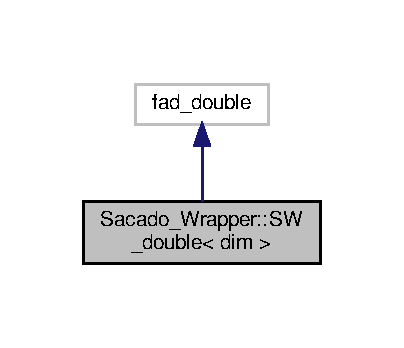
\includegraphics[width=194pt]{classSacado__Wrapper_1_1SW__double__inherit__graph}
\end{center}
\end{figure}


Collaboration diagram for Sacado\+\_\+\+Wrapper\+:\+:S\+W\+\_\+double$<$ dim $>$\+:\nopagebreak
\begin{figure}[H]
\begin{center}
\leavevmode
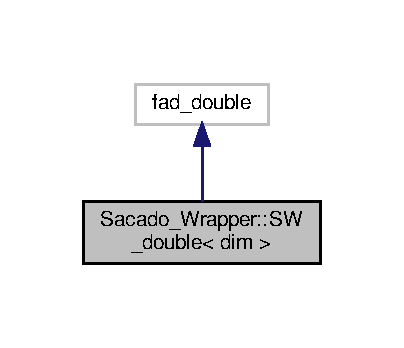
\includegraphics[width=194pt]{classSacado__Wrapper_1_1SW__double__coll__graph}
\end{center}
\end{figure}
\subsection*{Public Member Functions}
\begin{DoxyCompactItemize}
\item 
\hyperlink{classSacado__Wrapper_1_1SW__double}{S\+W\+\_\+double} \& \hyperlink{classSacado__Wrapper_1_1SW__double_a355de495ebe0e0b78ea4569fbb697717}{operator=} (double double\+\_\+init)
\item 
\hyperlink{classSacado__Wrapper_1_1SW__double}{S\+W\+\_\+double} \& \hyperlink{classSacado__Wrapper_1_1SW__double_ae9d242c29208f994f2eaabd9f5d5fa3c}{operator=} (\hyperlink{Sacado__example_8cc_a868b94676739e612d9c95940e70892a9}{fad\+\_\+double} fad\+\_\+assignment)
\item 
void \hyperlink{classSacado__Wrapper_1_1SW__double_adca799dd92dadebda9aebc91c797682a}{init} (const double \&double\+\_\+init)
\item 
void \hyperlink{classSacado__Wrapper_1_1SW__double_a36ced4218d40104fd8e548039a97cfb8}{set\+\_\+dofs} (unsigned \hyperlink{CMakeCache_8txt_a79a3d8790b2588b09777910863574e09}{int} nbr\+\_\+total\+\_\+dofs=\hyperlink{classSacado__Wrapper_1_1SW__double_a45e46904e5fd5be42bb4c9bb7454ffc5}{n\+\_\+dofs})
\item 
void \hyperlink{classSacado__Wrapper_1_1SW__double_a2e6eca4457eb22b06172bb5749038f1e}{get\+\_\+tangent} (Symmetric\+Tensor$<$ 2, dim $>$ \&Tangent, Symmetric\+Tensor$<$ 2, dim, \hyperlink{Sacado__example_8cc_a868b94676739e612d9c95940e70892a9}{fad\+\_\+double} $>$ \&sigma)
\item 
void \hyperlink{classSacado__Wrapper_1_1SW__double_a468303caab70c91f72bfe0547afff53a}{get\+\_\+tangent} (double \&Tangent, \hyperlink{Sacado__example_8cc_a868b94676739e612d9c95940e70892a9}{fad\+\_\+double} \&argument)
\item 
void \hyperlink{classSacado__Wrapper_1_1SW__double_ae7e9f33604ea736e485576447d78a46c}{get\+\_\+values} (double \&return\+\_\+double)
\end{DoxyCompactItemize}
\subsection*{Public Attributes}
\begin{DoxyCompactItemize}
\item 
unsigned \hyperlink{CMakeCache_8txt_a79a3d8790b2588b09777910863574e09}{int} \hyperlink{classSacado__Wrapper_1_1SW__double_aa0927ce06528899dd44afe5d770840c1}{start\+\_\+index} = 0
\end{DoxyCompactItemize}
\subsection*{Static Public Attributes}
\begin{DoxyCompactItemize}
\item 
static const unsigned \hyperlink{CMakeCache_8txt_a79a3d8790b2588b09777910863574e09}{int} \hyperlink{classSacado__Wrapper_1_1SW__double_a45e46904e5fd5be42bb4c9bb7454ffc5}{n\+\_\+dofs} = 1
\end{DoxyCompactItemize}


\subsection{Member Function Documentation}
\index{Sacado\+\_\+\+Wrapper\+::\+S\+W\+\_\+double@{Sacado\+\_\+\+Wrapper\+::\+S\+W\+\_\+double}!get\+\_\+tangent@{get\+\_\+tangent}}
\index{get\+\_\+tangent@{get\+\_\+tangent}!Sacado\+\_\+\+Wrapper\+::\+S\+W\+\_\+double@{Sacado\+\_\+\+Wrapper\+::\+S\+W\+\_\+double}}
\subsubsection[{\texorpdfstring{get\+\_\+tangent(\+Symmetric\+Tensor$<$ 2, dim $>$ \&\+Tangent, Symmetric\+Tensor$<$ 2, dim, fad\+\_\+double $>$ \&sigma)}{get_tangent(SymmetricTensor< 2, dim > &Tangent, SymmetricTensor< 2, dim, fad_double > &sigma)}}]{\setlength{\rightskip}{0pt plus 5cm}template$<$int dim$>$ void {\bf Sacado\+\_\+\+Wrapper\+::\+S\+W\+\_\+double}$<$ dim $>$\+::get\+\_\+tangent (
\begin{DoxyParamCaption}
\item[{Symmetric\+Tensor$<$ 2, dim $>$ \&}]{Tangent, }
\item[{Symmetric\+Tensor$<$ 2, dim, {\bf fad\+\_\+double} $>$ \&}]{sigma}
\end{DoxyParamCaption}
)}\hypertarget{classSacado__Wrapper_1_1SW__double_a2e6eca4457eb22b06172bb5749038f1e}{}\label{classSacado__Wrapper_1_1SW__double_a2e6eca4457eb22b06172bb5749038f1e}


Referenced by sacado\+\_\+test\+\_\+4().


\begin{DoxyCode}
358     \{
359         \textcolor{comment}{// reassemble the tangent as a SECOND order tensor}
360          \textcolor{keywordflow}{for} ( \textcolor{keywordtype}{unsigned} \textcolor{keywordtype}{int} i=0; i<dim; ++i)
361             \textcolor{keywordflow}{for} ( \textcolor{keywordtype}{unsigned} \textcolor{keywordtype}{int} j=0; j<dim; ++j )
362             \{
363                 \textcolor{keywordtype}{double} *derivs = &sigma[i][j].fastAccessDx(0); \textcolor{comment}{// Access derivatives}
364                 Tangent[i][j] = derivs[ this->\hyperlink{classSacado__Wrapper_1_1SW__double_aa0927ce06528899dd44afe5d770840c1}{start\_index} ]; \textcolor{comment}{// ToDo: check whether the 0.5* is
       necessary here too}
365             \}
366     \}
\end{DoxyCode}
\index{Sacado\+\_\+\+Wrapper\+::\+S\+W\+\_\+double@{Sacado\+\_\+\+Wrapper\+::\+S\+W\+\_\+double}!get\+\_\+tangent@{get\+\_\+tangent}}
\index{get\+\_\+tangent@{get\+\_\+tangent}!Sacado\+\_\+\+Wrapper\+::\+S\+W\+\_\+double@{Sacado\+\_\+\+Wrapper\+::\+S\+W\+\_\+double}}
\subsubsection[{\texorpdfstring{get\+\_\+tangent(double \&\+Tangent, fad\+\_\+double \&argument)}{get_tangent(double &Tangent, fad_double &argument)}}]{\setlength{\rightskip}{0pt plus 5cm}template$<$int dim$>$ void {\bf Sacado\+\_\+\+Wrapper\+::\+S\+W\+\_\+double}$<$ dim $>$\+::get\+\_\+tangent (
\begin{DoxyParamCaption}
\item[{double \&}]{Tangent, }
\item[{{\bf fad\+\_\+double} \&}]{argument}
\end{DoxyParamCaption}
)}\hypertarget{classSacado__Wrapper_1_1SW__double_a468303caab70c91f72bfe0547afff53a}{}\label{classSacado__Wrapper_1_1SW__double_a468303caab70c91f72bfe0547afff53a}

\begin{DoxyCode}
370     \{
371          \textcolor{keywordtype}{double} *derivs = &argument.fastAccessDx(0);
372          Tangent = derivs[ this->\hyperlink{classSacado__Wrapper_1_1SW__double_aa0927ce06528899dd44afe5d770840c1}{start\_index} ];
373     \}
\end{DoxyCode}
\index{Sacado\+\_\+\+Wrapper\+::\+S\+W\+\_\+double@{Sacado\+\_\+\+Wrapper\+::\+S\+W\+\_\+double}!get\+\_\+values@{get\+\_\+values}}
\index{get\+\_\+values@{get\+\_\+values}!Sacado\+\_\+\+Wrapper\+::\+S\+W\+\_\+double@{Sacado\+\_\+\+Wrapper\+::\+S\+W\+\_\+double}}
\subsubsection[{\texorpdfstring{get\+\_\+values(double \&return\+\_\+double)}{get_values(double &return_double)}}]{\setlength{\rightskip}{0pt plus 5cm}template$<$int dim$>$ void {\bf Sacado\+\_\+\+Wrapper\+::\+S\+W\+\_\+double}$<$ dim $>$\+::get\+\_\+values (
\begin{DoxyParamCaption}
\item[{double \&}]{return\+\_\+double}
\end{DoxyParamCaption}
)}\hypertarget{classSacado__Wrapper_1_1SW__double_ae7e9f33604ea736e485576447d78a46c}{}\label{classSacado__Wrapper_1_1SW__double_ae7e9f33604ea736e485576447d78a46c}

\begin{DoxyCode}
377     \{
378         return\_double = (*this).val();
379     \}
\end{DoxyCode}
\index{Sacado\+\_\+\+Wrapper\+::\+S\+W\+\_\+double@{Sacado\+\_\+\+Wrapper\+::\+S\+W\+\_\+double}!init@{init}}
\index{init@{init}!Sacado\+\_\+\+Wrapper\+::\+S\+W\+\_\+double@{Sacado\+\_\+\+Wrapper\+::\+S\+W\+\_\+double}}
\subsubsection[{\texorpdfstring{init(const double \&double\+\_\+init)}{init(const double &double_init)}}]{\setlength{\rightskip}{0pt plus 5cm}template$<$int dim$>$ void {\bf Sacado\+\_\+\+Wrapper\+::\+S\+W\+\_\+double}$<$ dim $>$\+::init (
\begin{DoxyParamCaption}
\item[{const double \&}]{double\+\_\+init}
\end{DoxyParamCaption}
)}\hypertarget{classSacado__Wrapper_1_1SW__double_adca799dd92dadebda9aebc91c797682a}{}\label{classSacado__Wrapper_1_1SW__double_adca799dd92dadebda9aebc91c797682a}


Referenced by sacado\+\_\+test\+\_\+4().


\begin{DoxyCode}
346     \{
347         (*this) = double\_init;
348     \}
\end{DoxyCode}
\index{Sacado\+\_\+\+Wrapper\+::\+S\+W\+\_\+double@{Sacado\+\_\+\+Wrapper\+::\+S\+W\+\_\+double}!operator=@{operator=}}
\index{operator=@{operator=}!Sacado\+\_\+\+Wrapper\+::\+S\+W\+\_\+double@{Sacado\+\_\+\+Wrapper\+::\+S\+W\+\_\+double}}
\subsubsection[{\texorpdfstring{operator=(double double\+\_\+init)}{operator=(double double_init)}}]{\setlength{\rightskip}{0pt plus 5cm}template$<$int dim$>$ {\bf S\+W\+\_\+double}\& {\bf Sacado\+\_\+\+Wrapper\+::\+S\+W\+\_\+double}$<$ dim $>$\+::operator= (
\begin{DoxyParamCaption}
\item[{double}]{double\+\_\+init}
\end{DoxyParamCaption}
)\hspace{0.3cm}{\ttfamily [inline]}}\hypertarget{classSacado__Wrapper_1_1SW__double_a355de495ebe0e0b78ea4569fbb697717}{}\label{classSacado__Wrapper_1_1SW__double_a355de495ebe0e0b78ea4569fbb697717}

\begin{DoxyCode}
327 \{ fad\_double::operator =( double\_init ) ;\textcolor{keywordflow}{return} *\textcolor{keyword}{this};\}
\end{DoxyCode}
\index{Sacado\+\_\+\+Wrapper\+::\+S\+W\+\_\+double@{Sacado\+\_\+\+Wrapper\+::\+S\+W\+\_\+double}!operator=@{operator=}}
\index{operator=@{operator=}!Sacado\+\_\+\+Wrapper\+::\+S\+W\+\_\+double@{Sacado\+\_\+\+Wrapper\+::\+S\+W\+\_\+double}}
\subsubsection[{\texorpdfstring{operator=(fad\+\_\+double fad\+\_\+assignment)}{operator=(fad_double fad_assignment)}}]{\setlength{\rightskip}{0pt plus 5cm}template$<$int dim$>$ {\bf S\+W\+\_\+double}\& {\bf Sacado\+\_\+\+Wrapper\+::\+S\+W\+\_\+double}$<$ dim $>$\+::operator= (
\begin{DoxyParamCaption}
\item[{{\bf fad\+\_\+double}}]{fad\+\_\+assignment}
\end{DoxyParamCaption}
)\hspace{0.3cm}{\ttfamily [inline]}}\hypertarget{classSacado__Wrapper_1_1SW__double_ae9d242c29208f994f2eaabd9f5d5fa3c}{}\label{classSacado__Wrapper_1_1SW__double_ae9d242c29208f994f2eaabd9f5d5fa3c}

\begin{DoxyCode}
328 \{ fad\_double::operator =( fad\_assignment ) ;\textcolor{keywordflow}{return} *\textcolor{keyword}{this};\}
\end{DoxyCode}
\index{Sacado\+\_\+\+Wrapper\+::\+S\+W\+\_\+double@{Sacado\+\_\+\+Wrapper\+::\+S\+W\+\_\+double}!set\+\_\+dofs@{set\+\_\+dofs}}
\index{set\+\_\+dofs@{set\+\_\+dofs}!Sacado\+\_\+\+Wrapper\+::\+S\+W\+\_\+double@{Sacado\+\_\+\+Wrapper\+::\+S\+W\+\_\+double}}
\subsubsection[{\texorpdfstring{set\+\_\+dofs(unsigned int nbr\+\_\+total\+\_\+dofs=n\+\_\+dofs)}{set_dofs(unsigned int nbr_total_dofs=n_dofs)}}]{\setlength{\rightskip}{0pt plus 5cm}template$<$int dim$>$ void {\bf Sacado\+\_\+\+Wrapper\+::\+S\+W\+\_\+double}$<$ dim $>$\+::set\+\_\+dofs (
\begin{DoxyParamCaption}
\item[{unsigned {\bf int}}]{nbr\+\_\+total\+\_\+dofs = {\ttfamily {\bf n\+\_\+dofs}}}
\end{DoxyParamCaption}
)}\hypertarget{classSacado__Wrapper_1_1SW__double_a36ced4218d40104fd8e548039a97cfb8}{}\label{classSacado__Wrapper_1_1SW__double_a36ced4218d40104fd8e548039a97cfb8}


Referenced by Sacado\+\_\+\+Wrapper\+::\+Do\+Fs\+\_\+summary$<$ dim $>$\+::set\+\_\+dofs().


\begin{DoxyCode}
352     \{
353         (*this).diff( this->\hyperlink{classSacado__Wrapper_1_1SW__double_aa0927ce06528899dd44afe5d770840c1}{start\_index}, nbr\_total\_dofs );
354     \}
\end{DoxyCode}


\subsection{Member Data Documentation}
\index{Sacado\+\_\+\+Wrapper\+::\+S\+W\+\_\+double@{Sacado\+\_\+\+Wrapper\+::\+S\+W\+\_\+double}!n\+\_\+dofs@{n\+\_\+dofs}}
\index{n\+\_\+dofs@{n\+\_\+dofs}!Sacado\+\_\+\+Wrapper\+::\+S\+W\+\_\+double@{Sacado\+\_\+\+Wrapper\+::\+S\+W\+\_\+double}}
\subsubsection[{\texorpdfstring{n\+\_\+dofs}{n_dofs}}]{\setlength{\rightskip}{0pt plus 5cm}template$<$int dim$>$ const unsigned {\bf int} {\bf Sacado\+\_\+\+Wrapper\+::\+S\+W\+\_\+double}$<$ dim $>$\+::n\+\_\+dofs = 1\hspace{0.3cm}{\ttfamily [static]}}\hypertarget{classSacado__Wrapper_1_1SW__double_a45e46904e5fd5be42bb4c9bb7454ffc5}{}\label{classSacado__Wrapper_1_1SW__double_a45e46904e5fd5be42bb4c9bb7454ffc5}


Referenced by Sacado\+\_\+\+Wrapper\+::\+Do\+Fs\+\_\+summary$<$ dim $>$\+::set\+\_\+dofs().

\index{Sacado\+\_\+\+Wrapper\+::\+S\+W\+\_\+double@{Sacado\+\_\+\+Wrapper\+::\+S\+W\+\_\+double}!start\+\_\+index@{start\+\_\+index}}
\index{start\+\_\+index@{start\+\_\+index}!Sacado\+\_\+\+Wrapper\+::\+S\+W\+\_\+double@{Sacado\+\_\+\+Wrapper\+::\+S\+W\+\_\+double}}
\subsubsection[{\texorpdfstring{start\+\_\+index}{start_index}}]{\setlength{\rightskip}{0pt plus 5cm}template$<$int dim$>$ unsigned {\bf int} {\bf Sacado\+\_\+\+Wrapper\+::\+S\+W\+\_\+double}$<$ dim $>$\+::start\+\_\+index = 0}\hypertarget{classSacado__Wrapper_1_1SW__double_aa0927ce06528899dd44afe5d770840c1}{}\label{classSacado__Wrapper_1_1SW__double_aa0927ce06528899dd44afe5d770840c1}


Referenced by Sacado\+\_\+\+Wrapper\+::\+Do\+Fs\+\_\+summary$<$ dim $>$\+::set\+\_\+dofs().



The documentation for this class was generated from the following file\+:\begin{DoxyCompactItemize}
\item 
\hyperlink{Sacado__Wrapper_8h}{Sacado\+\_\+\+Wrapper.\+h}\end{DoxyCompactItemize}

\hypertarget{classSacado__Wrapper_1_1SW__double2}{}\section{Sacado\+\_\+\+Wrapper\+:\+:S\+W\+\_\+double2$<$ dim $>$ Class Template Reference}
\label{classSacado__Wrapper_1_1SW__double2}\index{Sacado\+\_\+\+Wrapper\+::\+S\+W\+\_\+double2$<$ dim $>$@{Sacado\+\_\+\+Wrapper\+::\+S\+W\+\_\+double2$<$ dim $>$}}


{\ttfamily \#include $<$Sacado\+\_\+\+Wrapper.\+h$>$}



Inheritance diagram for Sacado\+\_\+\+Wrapper\+:\+:S\+W\+\_\+double2$<$ dim $>$\+:\nopagebreak
\begin{figure}[H]
\begin{center}
\leavevmode
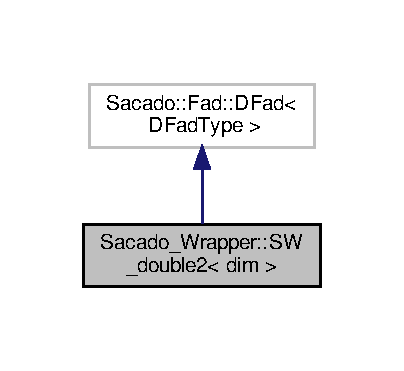
\includegraphics[width=194pt]{classSacado__Wrapper_1_1SW__double2__inherit__graph}
\end{center}
\end{figure}


Collaboration diagram for Sacado\+\_\+\+Wrapper\+:\+:S\+W\+\_\+double2$<$ dim $>$\+:\nopagebreak
\begin{figure}[H]
\begin{center}
\leavevmode
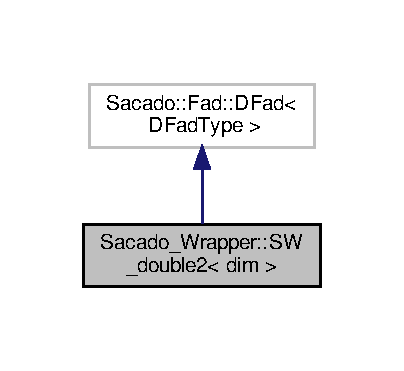
\includegraphics[width=194pt]{classSacado__Wrapper_1_1SW__double2__coll__graph}
\end{center}
\end{figure}
\subsection*{Public Member Functions}
\begin{DoxyCompactItemize}
\item 
\hyperlink{classSacado__Wrapper_1_1SW__double2}{S\+W\+\_\+double2} \& \hyperlink{classSacado__Wrapper_1_1SW__double2_a6f0538f891bd49efa54cc508da477f2e}{operator=} (double double\+\_\+init)
\item 
\hyperlink{classSacado__Wrapper_1_1SW__double2}{S\+W\+\_\+double2} \& \hyperlink{classSacado__Wrapper_1_1SW__double2_a426ab490411a347540e5af7028638495}{operator=} (Sacado\+::\+Fad\+::\+D\+Fad$<$ \hyperlink{Sacado__Wrapper_8h_a7e0893207b87dad05c66a34baac8ed2e}{D\+Fad\+Type} $>$ fad\+\_\+assignment)
\item 
void \hyperlink{classSacado__Wrapper_1_1SW__double2_af633ef0195198f1fed2bb44106af33c5}{init\+\_\+set\+\_\+dofs} (const double \&double\+\_\+init, unsigned \hyperlink{CMakeCache_8txt_a79a3d8790b2588b09777910863574e09}{int} nbr\+\_\+total\+\_\+dofs=\hyperlink{classSacado__Wrapper_1_1SW__double2_a535aa77392e896e21151bfc63f92e020}{n\+\_\+dofs})
\item 
void \hyperlink{classSacado__Wrapper_1_1SW__double2_ad51ba1e79171d60861b28098dfef903d}{get\+\_\+tangent} (double \&Tangent, Sacado\+::\+Fad\+::\+D\+Fad$<$ \hyperlink{Sacado__Wrapper_8h_a7e0893207b87dad05c66a34baac8ed2e}{D\+Fad\+Type} $>$ \&argument)
\item 
void \hyperlink{classSacado__Wrapper_1_1SW__double2_a9ee087929024da3da05268d5d0d4964b}{get\+\_\+tangent} (Symmetric\+Tensor$<$ 2, dim $>$ \&Tangent, Symmetric\+Tensor$<$ 2, dim, Sacado\+::\+Fad\+::\+D\+Fad$<$ \hyperlink{Sacado__Wrapper_8h_a7e0893207b87dad05c66a34baac8ed2e}{D\+Fad\+Type} $>$ $>$ \&argument, \hyperlink{classSacado__Wrapper_1_1SymTensor2}{Sym\+Tensor2}$<$ dim $>$ \&eps)
\item 
void \hyperlink{classSacado__Wrapper_1_1SW__double2_a7d3f3a21cd842645af9861bf50308825}{get\+\_\+curvature} (double \&Curvature, Sacado\+::\+Fad\+::\+D\+Fad$<$ \hyperlink{Sacado__Wrapper_8h_a7e0893207b87dad05c66a34baac8ed2e}{D\+Fad\+Type} $>$ \&argument)
\item 
void \hyperlink{classSacado__Wrapper_1_1SW__double2_a21da9eedb0c0e0d7db441426a5519a1a}{get\+\_\+curvature} (Symmetric\+Tensor$<$ 2, dim $>$ \&Curvature, Symmetric\+Tensor$<$ 2, dim, Sacado\+::\+Fad\+::\+D\+Fad$<$ \hyperlink{Sacado__Wrapper_8h_a7e0893207b87dad05c66a34baac8ed2e}{D\+Fad\+Type} $>$ $>$ \&argument, \hyperlink{classSacado__Wrapper_1_1SymTensor2}{Sym\+Tensor2}$<$ dim $>$ \&eps)
\item 
void \hyperlink{classSacado__Wrapper_1_1SW__double2_ac99cef52c5af3c6516aecf940275c595}{get\+\_\+curvature} (Symmetric\+Tensor$<$ 2, dim $>$ \&Curvature, Sacado\+::\+Fad\+::\+D\+Fad$<$ \hyperlink{Sacado__Wrapper_8h_a7e0893207b87dad05c66a34baac8ed2e}{D\+Fad\+Type} $>$ \&argument, \hyperlink{classSacado__Wrapper_1_1SymTensor2}{Sym\+Tensor2}$<$ dim $>$ \&eps)
\end{DoxyCompactItemize}
\subsection*{Public Attributes}
\begin{DoxyCompactItemize}
\item 
unsigned \hyperlink{CMakeCache_8txt_a79a3d8790b2588b09777910863574e09}{int} \hyperlink{classSacado__Wrapper_1_1SW__double2_ae7327540ad1fd725ea78ffc2268b423a}{start\+\_\+index} = 0
\end{DoxyCompactItemize}
\subsection*{Static Public Attributes}
\begin{DoxyCompactItemize}
\item 
static const unsigned \hyperlink{CMakeCache_8txt_a79a3d8790b2588b09777910863574e09}{int} \hyperlink{classSacado__Wrapper_1_1SW__double2_a535aa77392e896e21151bfc63f92e020}{n\+\_\+dofs} = 1
\end{DoxyCompactItemize}


\subsection{Member Function Documentation}
\index{Sacado\+\_\+\+Wrapper\+::\+S\+W\+\_\+double2@{Sacado\+\_\+\+Wrapper\+::\+S\+W\+\_\+double2}!get\+\_\+curvature@{get\+\_\+curvature}}
\index{get\+\_\+curvature@{get\+\_\+curvature}!Sacado\+\_\+\+Wrapper\+::\+S\+W\+\_\+double2@{Sacado\+\_\+\+Wrapper\+::\+S\+W\+\_\+double2}}
\subsubsection[{\texorpdfstring{get\+\_\+curvature(double \&\+Curvature, Sacado\+::\+Fad\+::\+D\+Fad$<$ D\+Fad\+Type $>$ \&argument)}{get_curvature(double &Curvature, Sacado::Fad::DFad< DFadType > &argument)}}]{\setlength{\rightskip}{0pt plus 5cm}template$<$int dim$>$ void {\bf Sacado\+\_\+\+Wrapper\+::\+S\+W\+\_\+double2}$<$ dim $>$\+::get\+\_\+curvature (
\begin{DoxyParamCaption}
\item[{double \&}]{Curvature, }
\item[{Sacado\+::\+Fad\+::\+D\+Fad$<$ {\bf D\+Fad\+Type} $>$ \&}]{argument}
\end{DoxyParamCaption}
)}\hypertarget{classSacado__Wrapper_1_1SW__double2_a7d3f3a21cd842645af9861bf50308825}{}\label{classSacado__Wrapper_1_1SW__double2_a7d3f3a21cd842645af9861bf50308825}


Referenced by Sacado\+\_\+\+Wrapper\+::\+Do\+Fs\+\_\+summary$<$ dim $>$\+::get\+\_\+curvature(), and sacado\+\_\+test\+\_\+8().


\begin{DoxyCode}
451     \{
452         Curvature = argument.dx(this->\hyperlink{classSacado__Wrapper_1_1SW__double2_ae7327540ad1fd725ea78ffc2268b423a}{start\_index}).dx(this->
      \hyperlink{classSacado__Wrapper_1_1SW__double2_ae7327540ad1fd725ea78ffc2268b423a}{start\_index});
453     \}
\end{DoxyCode}
\index{Sacado\+\_\+\+Wrapper\+::\+S\+W\+\_\+double2@{Sacado\+\_\+\+Wrapper\+::\+S\+W\+\_\+double2}!get\+\_\+curvature@{get\+\_\+curvature}}
\index{get\+\_\+curvature@{get\+\_\+curvature}!Sacado\+\_\+\+Wrapper\+::\+S\+W\+\_\+double2@{Sacado\+\_\+\+Wrapper\+::\+S\+W\+\_\+double2}}
\subsubsection[{\texorpdfstring{get\+\_\+curvature(\+Symmetric\+Tensor$<$ 2, dim $>$ \&\+Curvature, Symmetric\+Tensor$<$ 2, dim, Sacado\+::\+Fad\+::\+D\+Fad$<$ D\+Fad\+Type $>$ $>$ \&argument, Sym\+Tensor2$<$ dim $>$ \&eps)}{get_curvature(SymmetricTensor< 2, dim > &Curvature, SymmetricTensor< 2, dim, Sacado::Fad::DFad< DFadType > > &argument, SymTensor2< dim > &eps)}}]{\setlength{\rightskip}{0pt plus 5cm}template$<$int dim$>$ void {\bf Sacado\+\_\+\+Wrapper\+::\+S\+W\+\_\+double2}$<$ dim $>$\+::get\+\_\+curvature (
\begin{DoxyParamCaption}
\item[{Symmetric\+Tensor$<$ 2, dim $>$ \&}]{Curvature, }
\item[{Symmetric\+Tensor$<$ 2, dim, Sacado\+::\+Fad\+::\+D\+Fad$<$ {\bf D\+Fad\+Type} $>$ $>$ \&}]{argument, }
\item[{{\bf Sym\+Tensor2}$<$ dim $>$ \&}]{eps}
\end{DoxyParamCaption}
)}\hypertarget{classSacado__Wrapper_1_1SW__double2_a21da9eedb0c0e0d7db441426a5519a1a}{}\label{classSacado__Wrapper_1_1SW__double2_a21da9eedb0c0e0d7db441426a5519a1a}


References Sacado\+\_\+\+Wrapper\+::\+Sym\+Tensor2$<$ dim $>$\+::n\+\_\+dofs, and Sacado\+\_\+\+Wrapper\+::\+Sym\+Tensor2$<$ dim $>$\+::std\+\_\+map\+\_\+indicies.


\begin{DoxyCode}
461     \{
462         \textcolor{keywordflow}{for}(\textcolor{keywordtype}{unsigned} \textcolor{keywordtype}{int} x=0;x<eps.n\_dofs;++x)
463         \{
464             \textcolor{keyword}{const} \textcolor{keywordtype}{unsigned} \textcolor{keywordtype}{int} i=eps.std\_map\_indicies[x].first;
465             \textcolor{keyword}{const} \textcolor{keywordtype}{unsigned} \textcolor{keywordtype}{int} j=eps.std\_map\_indicies[x].second;
466 
467 \textcolor{comment}{//          if ( i!=j )}
468 \textcolor{comment}{//              Curvature[i][j] = 0.5 * argument[i][j].val().dx(start\_index);   // ToDo: check the factor
       0.5}
469 \textcolor{comment}{//          else}
470                 Curvature[i][j] = argument[i][j].val().dx(\hyperlink{classSacado__Wrapper_1_1SW__double2_ae7327540ad1fd725ea78ffc2268b423a}{start\_index});
471         \}
472     \}
\end{DoxyCode}
\index{Sacado\+\_\+\+Wrapper\+::\+S\+W\+\_\+double2@{Sacado\+\_\+\+Wrapper\+::\+S\+W\+\_\+double2}!get\+\_\+curvature@{get\+\_\+curvature}}
\index{get\+\_\+curvature@{get\+\_\+curvature}!Sacado\+\_\+\+Wrapper\+::\+S\+W\+\_\+double2@{Sacado\+\_\+\+Wrapper\+::\+S\+W\+\_\+double2}}
\subsubsection[{\texorpdfstring{get\+\_\+curvature(\+Symmetric\+Tensor$<$ 2, dim $>$ \&\+Curvature, Sacado\+::\+Fad\+::\+D\+Fad$<$ D\+Fad\+Type $>$ \&argument, Sym\+Tensor2$<$ dim $>$ \&eps)}{get_curvature(SymmetricTensor< 2, dim > &Curvature, Sacado::Fad::DFad< DFadType > &argument, SymTensor2< dim > &eps)}}]{\setlength{\rightskip}{0pt plus 5cm}template$<$int dim$>$ void {\bf Sacado\+\_\+\+Wrapper\+::\+S\+W\+\_\+double2}$<$ dim $>$\+::get\+\_\+curvature (
\begin{DoxyParamCaption}
\item[{Symmetric\+Tensor$<$ 2, dim $>$ \&}]{Curvature, }
\item[{Sacado\+::\+Fad\+::\+D\+Fad$<$ {\bf D\+Fad\+Type} $>$ \&}]{argument, }
\item[{{\bf Sym\+Tensor2}$<$ dim $>$ \&}]{eps}
\end{DoxyParamCaption}
)}\hypertarget{classSacado__Wrapper_1_1SW__double2_ac99cef52c5af3c6516aecf940275c595}{}\label{classSacado__Wrapper_1_1SW__double2_ac99cef52c5af3c6516aecf940275c595}


References Sacado\+\_\+\+Wrapper\+::\+Sym\+Tensor2$<$ dim $>$\+::n\+\_\+dofs, and Sacado\+\_\+\+Wrapper\+::\+Sym\+Tensor2$<$ dim $>$\+::std\+\_\+map\+\_\+indicies.


\begin{DoxyCode}
479     \{
480         \textcolor{keywordflow}{for}(\textcolor{keywordtype}{unsigned} \textcolor{keywordtype}{int} x=0;x<eps.n\_dofs;++x)
481         \{
482             \textcolor{keyword}{const} \textcolor{keywordtype}{unsigned} \textcolor{keywordtype}{int} i=eps.std\_map\_indicies[x].first;
483             \textcolor{keyword}{const} \textcolor{keywordtype}{unsigned} \textcolor{keywordtype}{int} j=eps.std\_map\_indicies[x].second;
484 
485             \textcolor{keywordflow}{if} ( i!=j )
486                 Curvature[i][j] = 0.5 * argument.dx(\hyperlink{classSacado__Wrapper_1_1SW__double2_ae7327540ad1fd725ea78ffc2268b423a}{start\_index}).dx(x);  \textcolor{comment}{// ToDo: check the
       factor 0.5}
487             \textcolor{keywordflow}{else}
488                 Curvature[i][j] = argument.dx(\hyperlink{classSacado__Wrapper_1_1SW__double2_ae7327540ad1fd725ea78ffc2268b423a}{start\_index}).dx(x);
489         \}
490     \}
\end{DoxyCode}
\index{Sacado\+\_\+\+Wrapper\+::\+S\+W\+\_\+double2@{Sacado\+\_\+\+Wrapper\+::\+S\+W\+\_\+double2}!get\+\_\+tangent@{get\+\_\+tangent}}
\index{get\+\_\+tangent@{get\+\_\+tangent}!Sacado\+\_\+\+Wrapper\+::\+S\+W\+\_\+double2@{Sacado\+\_\+\+Wrapper\+::\+S\+W\+\_\+double2}}
\subsubsection[{\texorpdfstring{get\+\_\+tangent(double \&\+Tangent, Sacado\+::\+Fad\+::\+D\+Fad$<$ D\+Fad\+Type $>$ \&argument)}{get_tangent(double &Tangent, Sacado::Fad::DFad< DFadType > &argument)}}]{\setlength{\rightskip}{0pt plus 5cm}template$<$int dim$>$ void {\bf Sacado\+\_\+\+Wrapper\+::\+S\+W\+\_\+double2}$<$ dim $>$\+::get\+\_\+tangent (
\begin{DoxyParamCaption}
\item[{double \&}]{Tangent, }
\item[{Sacado\+::\+Fad\+::\+D\+Fad$<$ {\bf D\+Fad\+Type} $>$ \&}]{argument}
\end{DoxyParamCaption}
)}\hypertarget{classSacado__Wrapper_1_1SW__double2_ad51ba1e79171d60861b28098dfef903d}{}\label{classSacado__Wrapper_1_1SW__double2_ad51ba1e79171d60861b28098dfef903d}


Referenced by sacado\+\_\+test\+\_\+8().


\begin{DoxyCode}
431     \{
432         Tangent = argument.dx(this->\hyperlink{classSacado__Wrapper_1_1SW__double2_ae7327540ad1fd725ea78ffc2268b423a}{start\_index}).val();
433     \}
\end{DoxyCode}
\index{Sacado\+\_\+\+Wrapper\+::\+S\+W\+\_\+double2@{Sacado\+\_\+\+Wrapper\+::\+S\+W\+\_\+double2}!get\+\_\+tangent@{get\+\_\+tangent}}
\index{get\+\_\+tangent@{get\+\_\+tangent}!Sacado\+\_\+\+Wrapper\+::\+S\+W\+\_\+double2@{Sacado\+\_\+\+Wrapper\+::\+S\+W\+\_\+double2}}
\subsubsection[{\texorpdfstring{get\+\_\+tangent(\+Symmetric\+Tensor$<$ 2, dim $>$ \&\+Tangent, Symmetric\+Tensor$<$ 2, dim, Sacado\+::\+Fad\+::\+D\+Fad$<$ D\+Fad\+Type $>$ $>$ \&argument, Sym\+Tensor2$<$ dim $>$ \&eps)}{get_tangent(SymmetricTensor< 2, dim > &Tangent, SymmetricTensor< 2, dim, Sacado::Fad::DFad< DFadType > > &argument, SymTensor2< dim > &eps)}}]{\setlength{\rightskip}{0pt plus 5cm}template$<$int dim$>$ void {\bf Sacado\+\_\+\+Wrapper\+::\+S\+W\+\_\+double2}$<$ dim $>$\+::get\+\_\+tangent (
\begin{DoxyParamCaption}
\item[{Symmetric\+Tensor$<$ 2, dim $>$ \&}]{Tangent, }
\item[{Symmetric\+Tensor$<$ 2, dim, Sacado\+::\+Fad\+::\+D\+Fad$<$ {\bf D\+Fad\+Type} $>$ $>$ \&}]{argument, }
\item[{{\bf Sym\+Tensor2}$<$ dim $>$ \&}]{eps}
\end{DoxyParamCaption}
)}\hypertarget{classSacado__Wrapper_1_1SW__double2_a9ee087929024da3da05268d5d0d4964b}{}\label{classSacado__Wrapper_1_1SW__double2_a9ee087929024da3da05268d5d0d4964b}


References Sacado\+\_\+\+Wrapper\+::\+Sym\+Tensor2$<$ dim $>$\+::n\+\_\+dofs, and Sacado\+\_\+\+Wrapper\+::\+Sym\+Tensor2$<$ dim $>$\+::std\+\_\+map\+\_\+indicies.


\begin{DoxyCode}
438     \{
439         \textcolor{keywordflow}{for}(\textcolor{keywordtype}{unsigned} \textcolor{keywordtype}{int} x=0;x<eps.n\_dofs;++x)
440         \{
441             \textcolor{keyword}{const} \textcolor{keywordtype}{unsigned} \textcolor{keywordtype}{int} i=eps.std\_map\_indicies[x].first;
442             \textcolor{keyword}{const} \textcolor{keywordtype}{unsigned} \textcolor{keywordtype}{int} j=eps.std\_map\_indicies[x].second;
443             \textcolor{comment}{// ToDo: find a better way to loop over the indices than using eps as input argument}
444             Tangent[i][j] = argument[i][j].dx(\hyperlink{classSacado__Wrapper_1_1SW__double2_ae7327540ad1fd725ea78ffc2268b423a}{start\_index}).val();
445         \}
446     \}
\end{DoxyCode}
\index{Sacado\+\_\+\+Wrapper\+::\+S\+W\+\_\+double2@{Sacado\+\_\+\+Wrapper\+::\+S\+W\+\_\+double2}!init\+\_\+set\+\_\+dofs@{init\+\_\+set\+\_\+dofs}}
\index{init\+\_\+set\+\_\+dofs@{init\+\_\+set\+\_\+dofs}!Sacado\+\_\+\+Wrapper\+::\+S\+W\+\_\+double2@{Sacado\+\_\+\+Wrapper\+::\+S\+W\+\_\+double2}}
\subsubsection[{\texorpdfstring{init\+\_\+set\+\_\+dofs(const double \&double\+\_\+init, unsigned int nbr\+\_\+total\+\_\+dofs=n\+\_\+dofs)}{init_set_dofs(const double &double_init, unsigned int nbr_total_dofs=n_dofs)}}]{\setlength{\rightskip}{0pt plus 5cm}template$<$int dim$>$ void {\bf Sacado\+\_\+\+Wrapper\+::\+S\+W\+\_\+double2}$<$ dim $>$\+::init\+\_\+set\+\_\+dofs (
\begin{DoxyParamCaption}
\item[{const double \&}]{double\+\_\+init, }
\item[{unsigned {\bf int}}]{nbr\+\_\+total\+\_\+dofs = {\ttfamily {\bf n\+\_\+dofs}}}
\end{DoxyParamCaption}
)}\hypertarget{classSacado__Wrapper_1_1SW__double2_af633ef0195198f1fed2bb44106af33c5}{}\label{classSacado__Wrapper_1_1SW__double2_af633ef0195198f1fed2bb44106af33c5}


Referenced by Sacado\+\_\+\+Wrapper\+::\+Do\+Fs\+\_\+summary$<$ dim $>$\+::init\+\_\+set\+\_\+dofs().


\begin{DoxyCode}
423     \{
424         (*this).diff( \hyperlink{classSacado__Wrapper_1_1SW__double2_ae7327540ad1fd725ea78ffc2268b423a}{start\_index} , nbr\_total\_dofs );
425         (*this).val() = \hyperlink{Sacado__Wrapper_8h_a868b94676739e612d9c95940e70892a9}{fad\_double}(nbr\_total\_dofs, \hyperlink{classSacado__Wrapper_1_1SW__double2_ae7327540ad1fd725ea78ffc2268b423a}{start\_index}, double\_init);
426     \}
\end{DoxyCode}
\index{Sacado\+\_\+\+Wrapper\+::\+S\+W\+\_\+double2@{Sacado\+\_\+\+Wrapper\+::\+S\+W\+\_\+double2}!operator=@{operator=}}
\index{operator=@{operator=}!Sacado\+\_\+\+Wrapper\+::\+S\+W\+\_\+double2@{Sacado\+\_\+\+Wrapper\+::\+S\+W\+\_\+double2}}
\subsubsection[{\texorpdfstring{operator=(double double\+\_\+init)}{operator=(double double_init)}}]{\setlength{\rightskip}{0pt plus 5cm}template$<$int dim$>$ {\bf S\+W\+\_\+double2}\& {\bf Sacado\+\_\+\+Wrapper\+::\+S\+W\+\_\+double2}$<$ dim $>$\+::operator= (
\begin{DoxyParamCaption}
\item[{double}]{double\+\_\+init}
\end{DoxyParamCaption}
)\hspace{0.3cm}{\ttfamily [inline]}}\hypertarget{classSacado__Wrapper_1_1SW__double2_a6f0538f891bd49efa54cc508da477f2e}{}\label{classSacado__Wrapper_1_1SW__double2_a6f0538f891bd49efa54cc508da477f2e}

\begin{DoxyCode}
401 \{ Sacado::Fad::DFad<DFadType>::operator =( double\_init ) ;\textcolor{keywordflow}{return} *\textcolor{keyword}{this};\}
\end{DoxyCode}
\index{Sacado\+\_\+\+Wrapper\+::\+S\+W\+\_\+double2@{Sacado\+\_\+\+Wrapper\+::\+S\+W\+\_\+double2}!operator=@{operator=}}
\index{operator=@{operator=}!Sacado\+\_\+\+Wrapper\+::\+S\+W\+\_\+double2@{Sacado\+\_\+\+Wrapper\+::\+S\+W\+\_\+double2}}
\subsubsection[{\texorpdfstring{operator=(\+Sacado\+::\+Fad\+::\+D\+Fad$<$ D\+Fad\+Type $>$ fad\+\_\+assignment)}{operator=(Sacado::Fad::DFad< DFadType > fad_assignment)}}]{\setlength{\rightskip}{0pt plus 5cm}template$<$int dim$>$ {\bf S\+W\+\_\+double2}\& {\bf Sacado\+\_\+\+Wrapper\+::\+S\+W\+\_\+double2}$<$ dim $>$\+::operator= (
\begin{DoxyParamCaption}
\item[{Sacado\+::\+Fad\+::\+D\+Fad$<$ {\bf D\+Fad\+Type} $>$}]{fad\+\_\+assignment}
\end{DoxyParamCaption}
)\hspace{0.3cm}{\ttfamily [inline]}}\hypertarget{classSacado__Wrapper_1_1SW__double2_a426ab490411a347540e5af7028638495}{}\label{classSacado__Wrapper_1_1SW__double2_a426ab490411a347540e5af7028638495}

\begin{DoxyCode}
402 \{ Sacado::Fad::DFad<DFadType>::operator =( fad\_assignment ) ;\textcolor{keywordflow}{return} *\textcolor{keyword}{this};\}
\end{DoxyCode}


\subsection{Member Data Documentation}
\index{Sacado\+\_\+\+Wrapper\+::\+S\+W\+\_\+double2@{Sacado\+\_\+\+Wrapper\+::\+S\+W\+\_\+double2}!n\+\_\+dofs@{n\+\_\+dofs}}
\index{n\+\_\+dofs@{n\+\_\+dofs}!Sacado\+\_\+\+Wrapper\+::\+S\+W\+\_\+double2@{Sacado\+\_\+\+Wrapper\+::\+S\+W\+\_\+double2}}
\subsubsection[{\texorpdfstring{n\+\_\+dofs}{n_dofs}}]{\setlength{\rightskip}{0pt plus 5cm}template$<$int dim$>$ const unsigned {\bf int} {\bf Sacado\+\_\+\+Wrapper\+::\+S\+W\+\_\+double2}$<$ dim $>$\+::n\+\_\+dofs = 1\hspace{0.3cm}{\ttfamily [static]}}\hypertarget{classSacado__Wrapper_1_1SW__double2_a535aa77392e896e21151bfc63f92e020}{}\label{classSacado__Wrapper_1_1SW__double2_a535aa77392e896e21151bfc63f92e020}


Referenced by Sacado\+\_\+\+Wrapper\+::\+Do\+Fs\+\_\+summary$<$ dim $>$\+::init\+\_\+set\+\_\+dofs().

\index{Sacado\+\_\+\+Wrapper\+::\+S\+W\+\_\+double2@{Sacado\+\_\+\+Wrapper\+::\+S\+W\+\_\+double2}!start\+\_\+index@{start\+\_\+index}}
\index{start\+\_\+index@{start\+\_\+index}!Sacado\+\_\+\+Wrapper\+::\+S\+W\+\_\+double2@{Sacado\+\_\+\+Wrapper\+::\+S\+W\+\_\+double2}}
\subsubsection[{\texorpdfstring{start\+\_\+index}{start_index}}]{\setlength{\rightskip}{0pt plus 5cm}template$<$int dim$>$ unsigned {\bf int} {\bf Sacado\+\_\+\+Wrapper\+::\+S\+W\+\_\+double2}$<$ dim $>$\+::start\+\_\+index = 0}\hypertarget{classSacado__Wrapper_1_1SW__double2_ae7327540ad1fd725ea78ffc2268b423a}{}\label{classSacado__Wrapper_1_1SW__double2_ae7327540ad1fd725ea78ffc2268b423a}


Referenced by Sacado\+\_\+\+Wrapper\+::\+Do\+Fs\+\_\+summary$<$ dim $>$\+::init\+\_\+set\+\_\+dofs().



The documentation for this class was generated from the following file\+:\begin{DoxyCompactItemize}
\item 
\hyperlink{Sacado__Wrapper_8h}{Sacado\+\_\+\+Wrapper.\+h}\end{DoxyCompactItemize}

\hypertarget{classSacado__Wrapper_1_1SymTensor}{}\section{Sacado\+\_\+\+Wrapper\+:\+:Sym\+Tensor$<$ dim $>$ Class Template Reference}
\label{classSacado__Wrapper_1_1SymTensor}\index{Sacado\+\_\+\+Wrapper\+::\+Sym\+Tensor$<$ dim $>$@{Sacado\+\_\+\+Wrapper\+::\+Sym\+Tensor$<$ dim $>$}}


{\ttfamily \#include $<$Sacado\+\_\+\+Wrapper.\+h$>$}



Inheritance diagram for Sacado\+\_\+\+Wrapper\+:\+:Sym\+Tensor$<$ dim $>$\+:
\nopagebreak
\begin{figure}[H]
\begin{center}
\leavevmode
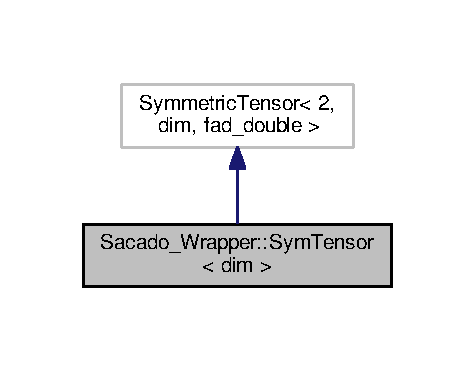
\includegraphics[width=228pt]{classSacado__Wrapper_1_1SymTensor__inherit__graph}
\end{center}
\end{figure}


Collaboration diagram for Sacado\+\_\+\+Wrapper\+:\+:Sym\+Tensor$<$ dim $>$\+:
\nopagebreak
\begin{figure}[H]
\begin{center}
\leavevmode
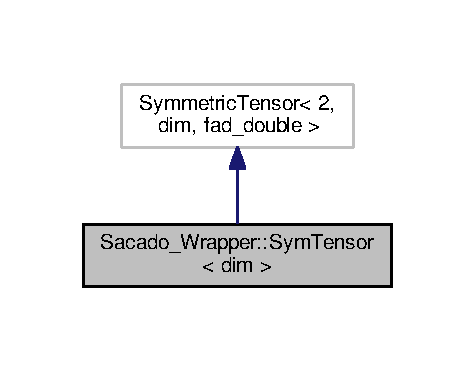
\includegraphics[width=228pt]{classSacado__Wrapper_1_1SymTensor__coll__graph}
\end{center}
\end{figure}
\subsection*{Public Member Functions}
\begin{DoxyCompactItemize}
\item 
\hyperlink{classSacado__Wrapper_1_1SymTensor_a4e7ec32177eb891e3f1a32a16bcd59f5}{Sym\+Tensor} ()
\item 
void \hyperlink{classSacado__Wrapper_1_1SymTensor_acbad579d5ead9e96ff46aa15d9b5aef4}{init} (Symmetric\+Tensor$<$ 2, dim $>$ \&tensor\+\_\+double)
\item 
void \hyperlink{classSacado__Wrapper_1_1SymTensor_ae5e13d654682e392f39dc0991bdd95a2}{set\+\_\+dofs} ()
\item 
void \hyperlink{classSacado__Wrapper_1_1SymTensor_ab97427c3b5cab279e58607cf431ab262}{get\+\_\+tangent} (Symmetric\+Tensor$<$ 4, dim $>$ \&Tangent, Symmetric\+Tensor$<$ 2, dim, \hyperlink{Sacado__example_8cc_a868b94676739e612d9c95940e70892a9}{fad\+\_\+double} $>$ \&sigma)
\end{DoxyCompactItemize}
\subsection*{Public Attributes}
\begin{DoxyCompactItemize}
\item 
std\+::map$<$ unsigned int, std\+::pair$<$ unsigned int, unsigned int $>$ $>$ \hyperlink{classSacado__Wrapper_1_1SymTensor_ae3b1c56cde3fc5c7805b618ef3d9de75}{std\+\_\+map\+\_\+indicies}
\end{DoxyCompactItemize}


\subsection{Constructor \& Destructor Documentation}
\index{Sacado\+\_\+\+Wrapper\+::\+Sym\+Tensor@{Sacado\+\_\+\+Wrapper\+::\+Sym\+Tensor}!Sym\+Tensor@{Sym\+Tensor}}
\index{Sym\+Tensor@{Sym\+Tensor}!Sacado\+\_\+\+Wrapper\+::\+Sym\+Tensor@{Sacado\+\_\+\+Wrapper\+::\+Sym\+Tensor}}
\subsubsection[{\texorpdfstring{Sym\+Tensor()}{SymTensor()}}]{\setlength{\rightskip}{0pt plus 5cm}template$<$int dim$>$ {\bf Sacado\+\_\+\+Wrapper\+::\+Sym\+Tensor}$<$ dim $>$\+::{\bf Sym\+Tensor} (
\begin{DoxyParamCaption}
{}
\end{DoxyParamCaption}
)\hspace{0.3cm}{\ttfamily [inline]}}\hypertarget{classSacado__Wrapper_1_1SymTensor_a4e7ec32177eb891e3f1a32a16bcd59f5}{}\label{classSacado__Wrapper_1_1SymTensor_a4e7ec32177eb891e3f1a32a16bcd59f5}

\begin{DoxyCode}
25         \{
26             std::pair<unsigned int, unsigned int> tmp\_pair;
27 
28             \textcolor{keywordflow}{switch} ( dim )
29             \{
30             \textcolor{keywordflow}{case} 2:
31                 tmp\_pair.first=0; tmp\_pair.second=0;
32                 \hyperlink{classSacado__Wrapper_1_1SymTensor_ae3b1c56cde3fc5c7805b618ef3d9de75}{std\_map\_indicies}[0] = tmp\_pair;
33                 
34                 tmp\_pair.first=0; tmp\_pair.second=1;
35                 \hyperlink{classSacado__Wrapper_1_1SymTensor_ae3b1c56cde3fc5c7805b618ef3d9de75}{std\_map\_indicies}[1] = tmp\_pair;
36                 
37                 tmp\_pair.first=1; tmp\_pair.second=1;
38                 \hyperlink{classSacado__Wrapper_1_1SymTensor_ae3b1c56cde3fc5c7805b618ef3d9de75}{std\_map\_indicies}[2] = tmp\_pair; 
39                 \textcolor{keywordflow}{break};
40             \textcolor{keywordflow}{case} 3:
41                 tmp\_pair.first=0; tmp\_pair.second=0;
42                 \hyperlink{classSacado__Wrapper_1_1SymTensor_ae3b1c56cde3fc5c7805b618ef3d9de75}{std\_map\_indicies}[0] = tmp\_pair;
43 
44                 tmp\_pair.first=0; tmp\_pair.second=1;
45                 \hyperlink{classSacado__Wrapper_1_1SymTensor_ae3b1c56cde3fc5c7805b618ef3d9de75}{std\_map\_indicies}[1] = tmp\_pair;
46 
47                 tmp\_pair.first=0; tmp\_pair.second=2;
48                 \hyperlink{classSacado__Wrapper_1_1SymTensor_ae3b1c56cde3fc5c7805b618ef3d9de75}{std\_map\_indicies}[2] = tmp\_pair;
49 
50                 tmp\_pair.first=1; tmp\_pair.second=1;
51                 \hyperlink{classSacado__Wrapper_1_1SymTensor_ae3b1c56cde3fc5c7805b618ef3d9de75}{std\_map\_indicies}[3] = tmp\_pair;
52 
53                 tmp\_pair.first=1; tmp\_pair.second=2;
54                 \hyperlink{classSacado__Wrapper_1_1SymTensor_ae3b1c56cde3fc5c7805b618ef3d9de75}{std\_map\_indicies}[4] = tmp\_pair;
55 
56                 tmp\_pair.first=2; tmp\_pair.second=2;
57                 \hyperlink{classSacado__Wrapper_1_1SymTensor_ae3b1c56cde3fc5c7805b618ef3d9de75}{std\_map\_indicies}[5] = tmp\_pair;
58                 \textcolor{keywordflow}{break};
59             \}
60         \}
\end{DoxyCode}


\subsection{Member Function Documentation}
\index{Sacado\+\_\+\+Wrapper\+::\+Sym\+Tensor@{Sacado\+\_\+\+Wrapper\+::\+Sym\+Tensor}!get\+\_\+tangent@{get\+\_\+tangent}}
\index{get\+\_\+tangent@{get\+\_\+tangent}!Sacado\+\_\+\+Wrapper\+::\+Sym\+Tensor@{Sacado\+\_\+\+Wrapper\+::\+Sym\+Tensor}}
\subsubsection[{\texorpdfstring{get\+\_\+tangent(\+Symmetric\+Tensor$<$ 4, dim $>$ \&\+Tangent, Symmetric\+Tensor$<$ 2, dim, fad\+\_\+double $>$ \&sigma)}{get_tangent(SymmetricTensor< 4, dim > &Tangent, SymmetricTensor< 2, dim, fad_double > &sigma)}}]{\setlength{\rightskip}{0pt plus 5cm}template$<$int dim$>$ void {\bf Sacado\+\_\+\+Wrapper\+::\+Sym\+Tensor}$<$ dim $>$\+::get\+\_\+tangent (
\begin{DoxyParamCaption}
\item[{Symmetric\+Tensor$<$ 4, dim $>$ \&}]{Tangent, }
\item[{Symmetric\+Tensor$<$ 2, dim, {\bf fad\+\_\+double} $>$ \&}]{sigma}
\end{DoxyParamCaption}
)}\hypertarget{classSacado__Wrapper_1_1SymTensor_ab97427c3b5cab279e58607cf431ab262}{}\label{classSacado__Wrapper_1_1SymTensor_ab97427c3b5cab279e58607cf431ab262}


Referenced by sacado\+\_\+test\+\_\+3\+B().


\begin{DoxyCode}
109     \{
110         \textcolor{keywordflow}{for} ( \textcolor{keywordtype}{unsigned} \textcolor{keywordtype}{int} i=0; i<dim; ++i)
111             \textcolor{keywordflow}{for} ( \textcolor{keywordtype}{unsigned} \textcolor{keywordtype}{int} j=0; j<dim; ++j )
112             \{
113                 \textcolor{keywordtype}{double} *derivs = &sigma[i][j].fastAccessDx(0); \textcolor{comment}{// Access the derivatives of the (i,j)-th
       component of \(\backslash\)a sigma}
114 
115                 \textcolor{comment}{// We loop over all the dofs. To be able to use this independent of the chosen dimension \(\backslash\)a
       dim, we use a ternary operator}
116                 \textcolor{comment}{// to decide whether we have to loop over 6 derivatives or just 3.}
117                 \textcolor{keywordflow}{for}(\textcolor{keywordtype}{unsigned} \textcolor{keywordtype}{int} x=0;x<((dim==2)?3:6);++x)
118                 \{
119                     \textcolor{keywordtype}{unsigned} \textcolor{keywordtype}{int} k=\hyperlink{classSacado__Wrapper_1_1SymTensor_ae3b1c56cde3fc5c7805b618ef3d9de75}{std\_map\_indicies}[x].first;
120                     \textcolor{keywordtype}{unsigned} \textcolor{keywordtype}{int} l=\hyperlink{classSacado__Wrapper_1_1SymTensor_ae3b1c56cde3fc5c7805b618ef3d9de75}{std\_map\_indicies}[x].second;
121 
122                     \textcolor{keywordflow}{if}(k!=l)\textcolor{comment}{/*Compare to Voigt notation since only SymmetricTensor instead of Tensor*/}
123                     \{
124                         Tangent[i][j][k][l] = 0.5*derivs[x];
125                         Tangent[i][j][l][k] = 0.5*derivs[x];
126                     \}
127                     \textcolor{keywordflow}{else}
128                         Tangent[i][j][k][l] = derivs[x];
129                 \}            
130             \}
131     \}
\end{DoxyCode}
\index{Sacado\+\_\+\+Wrapper\+::\+Sym\+Tensor@{Sacado\+\_\+\+Wrapper\+::\+Sym\+Tensor}!init@{init}}
\index{init@{init}!Sacado\+\_\+\+Wrapper\+::\+Sym\+Tensor@{Sacado\+\_\+\+Wrapper\+::\+Sym\+Tensor}}
\subsubsection[{\texorpdfstring{init(\+Symmetric\+Tensor$<$ 2, dim $>$ \&tensor\+\_\+double)}{init(SymmetricTensor< 2, dim > &tensor_double)}}]{\setlength{\rightskip}{0pt plus 5cm}template$<$int dim$>$ void {\bf Sacado\+\_\+\+Wrapper\+::\+Sym\+Tensor}$<$ dim $>$\+::init (
\begin{DoxyParamCaption}
\item[{Symmetric\+Tensor$<$ 2, dim $>$ \&}]{tensor\+\_\+double}
\end{DoxyParamCaption}
)}\hypertarget{classSacado__Wrapper_1_1SymTensor_acbad579d5ead9e96ff46aa15d9b5aef4}{}\label{classSacado__Wrapper_1_1SymTensor_acbad579d5ead9e96ff46aa15d9b5aef4}


Referenced by sacado\+\_\+test\+\_\+3\+B(), and sacado\+\_\+test\+\_\+4().


\begin{DoxyCode}
78     \{
79          \textcolor{keywordflow}{for} ( \textcolor{keywordtype}{unsigned} \textcolor{keywordtype}{int} i=0; i<dim; ++i)
80             \textcolor{keywordflow}{for} ( \textcolor{keywordtype}{unsigned} \textcolor{keywordtype}{int} j=0; j<dim; ++j )
81                 (*\textcolor{keyword}{this})[i][j] = tensor\_double[i][j];
82     \}
\end{DoxyCode}
\index{Sacado\+\_\+\+Wrapper\+::\+Sym\+Tensor@{Sacado\+\_\+\+Wrapper\+::\+Sym\+Tensor}!set\+\_\+dofs@{set\+\_\+dofs}}
\index{set\+\_\+dofs@{set\+\_\+dofs}!Sacado\+\_\+\+Wrapper\+::\+Sym\+Tensor@{Sacado\+\_\+\+Wrapper\+::\+Sym\+Tensor}}
\subsubsection[{\texorpdfstring{set\+\_\+dofs()}{set_dofs()}}]{\setlength{\rightskip}{0pt plus 5cm}template$<$int dim$>$ void {\bf Sacado\+\_\+\+Wrapper\+::\+Sym\+Tensor}$<$ dim $>$\+::set\+\_\+dofs (
\begin{DoxyParamCaption}
{}
\end{DoxyParamCaption}
)}\hypertarget{classSacado__Wrapper_1_1SymTensor_ae5e13d654682e392f39dc0991bdd95a2}{}\label{classSacado__Wrapper_1_1SymTensor_ae5e13d654682e392f39dc0991bdd95a2}


Referenced by sacado\+\_\+test\+\_\+3\+B(), and sacado\+\_\+test\+\_\+4().


\begin{DoxyCode}
90     \{
91         \textcolor{comment}{// Instead of calling the *.diff(*) on the components one-by-one we could also use the following
       for-loop, so}
92         \textcolor{comment}{// we also use the map to set the dofs}
93         \textcolor{keywordflow}{for} ( \textcolor{keywordtype}{unsigned} \textcolor{keywordtype}{int} x=0; x<((dim==2)?3:6); ++x )
94         \{
95             \textcolor{keywordtype}{unsigned} \textcolor{keywordtype}{int} i=\hyperlink{classSacado__Wrapper_1_1SymTensor_ae3b1c56cde3fc5c7805b618ef3d9de75}{std\_map\_indicies}[x].first;
96             \textcolor{keywordtype}{unsigned} \textcolor{keywordtype}{int} j=\hyperlink{classSacado__Wrapper_1_1SymTensor_ae3b1c56cde3fc5c7805b618ef3d9de75}{std\_map\_indicies}[x].second;
97             (*this)[i][j].diff(x,((dim==2)?3:6));
98         \}
99     \}
\end{DoxyCode}


\subsection{Member Data Documentation}
\index{Sacado\+\_\+\+Wrapper\+::\+Sym\+Tensor@{Sacado\+\_\+\+Wrapper\+::\+Sym\+Tensor}!std\+\_\+map\+\_\+indicies@{std\+\_\+map\+\_\+indicies}}
\index{std\+\_\+map\+\_\+indicies@{std\+\_\+map\+\_\+indicies}!Sacado\+\_\+\+Wrapper\+::\+Sym\+Tensor@{Sacado\+\_\+\+Wrapper\+::\+Sym\+Tensor}}
\subsubsection[{\texorpdfstring{std\+\_\+map\+\_\+indicies}{std_map_indicies}}]{\setlength{\rightskip}{0pt plus 5cm}template$<$int dim$>$ std\+::map$<$unsigned int,std\+::pair$<$unsigned int,unsigned int$>$ $>$ {\bf Sacado\+\_\+\+Wrapper\+::\+Sym\+Tensor}$<$ dim $>$\+::std\+\_\+map\+\_\+indicies}\hypertarget{classSacado__Wrapper_1_1SymTensor_ae3b1c56cde3fc5c7805b618ef3d9de75}{}\label{classSacado__Wrapper_1_1SymTensor_ae3b1c56cde3fc5c7805b618ef3d9de75}


The documentation for this class was generated from the following file\+:\begin{DoxyCompactItemize}
\item 
\hyperlink{Sacado__Wrapper_8h}{Sacado\+\_\+\+Wrapper.\+h}\end{DoxyCompactItemize}

\hypertarget{classSacado__Wrapper_1_1SymTensor2}{}\section{Sacado\+\_\+\+Wrapper\+:\+:Sym\+Tensor2$<$ dim $>$ Class Template Reference}
\label{classSacado__Wrapper_1_1SymTensor2}\index{Sacado\+\_\+\+Wrapper\+::\+Sym\+Tensor2$<$ dim $>$@{Sacado\+\_\+\+Wrapper\+::\+Sym\+Tensor2$<$ dim $>$}}


{\ttfamily \#include $<$Sacado\+\_\+\+Wrapper.\+h$>$}



Inheritance diagram for Sacado\+\_\+\+Wrapper\+:\+:Sym\+Tensor2$<$ dim $>$\+:
\nopagebreak
\begin{figure}[H]
\begin{center}
\leavevmode
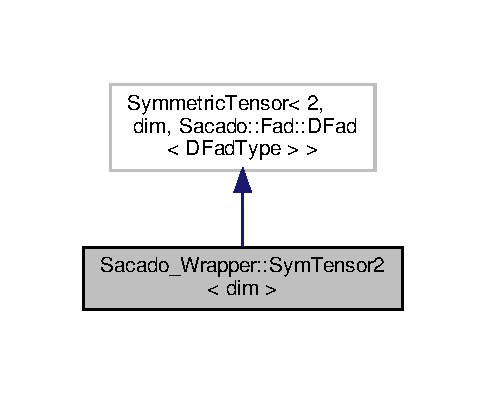
\includegraphics[width=233pt]{classSacado__Wrapper_1_1SymTensor2__inherit__graph}
\end{center}
\end{figure}


Collaboration diagram for Sacado\+\_\+\+Wrapper\+:\+:Sym\+Tensor2$<$ dim $>$\+:
\nopagebreak
\begin{figure}[H]
\begin{center}
\leavevmode
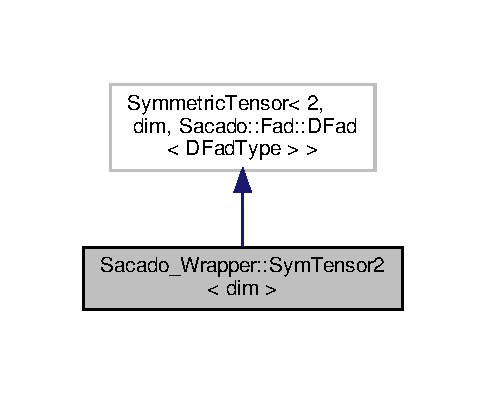
\includegraphics[width=233pt]{classSacado__Wrapper_1_1SymTensor2__coll__graph}
\end{center}
\end{figure}
\subsection*{Public Member Functions}
\begin{DoxyCompactItemize}
\item 
\hyperlink{classSacado__Wrapper_1_1SymTensor2_ae43e523ee18d7bf678e5d426df92cd49}{Sym\+Tensor2} ()
\item 
void \hyperlink{classSacado__Wrapper_1_1SymTensor2_a54495897cfdd887d0081015571a28107}{init\+\_\+set\+\_\+dofs} (Symmetric\+Tensor$<$ 2, dim $>$ \&tensor\+\_\+double, const unsigned \hyperlink{CMakeCache_8txt_a79a3d8790b2588b09777910863574e09}{int} nbr\+\_\+total\+\_\+dofs=\hyperlink{classSacado__Wrapper_1_1SymTensor2_ad9d6542de5481e0d41bd1831cb0aeaff}{n\+\_\+dofs})
\item 
void \hyperlink{classSacado__Wrapper_1_1SymTensor2_a4a7d1a0e9efb9d4a6bf6768a75611762}{get\+\_\+tangent} (Symmetric\+Tensor$<$ 4, dim $>$ \&Tangent, Symmetric\+Tensor$<$ 2, dim, Sacado\+::\+Fad\+::\+D\+Fad$<$ \hyperlink{Sacado__Wrapper_8h_a7e0893207b87dad05c66a34baac8ed2e}{D\+Fad\+Type} $>$ $>$ \&sigma)
\item 
void \hyperlink{classSacado__Wrapper_1_1SymTensor2_aad13518e282739f93126adb9db351474}{get\+\_\+tangent} (Symmetric\+Tensor$<$ 2, dim $>$ \&Tangent, Sacado\+::\+Fad\+::\+D\+Fad$<$ \hyperlink{Sacado__Wrapper_8h_a7e0893207b87dad05c66a34baac8ed2e}{D\+Fad\+Type} $>$ \&argument)
\item 
void \hyperlink{classSacado__Wrapper_1_1SymTensor2_a7cd555be3d8c00559af7954671f417fa}{get\+\_\+tangent} (Symmetric\+Tensor$<$ 2, dim, Sacado\+::\+Fad\+::\+D\+Fad$<$ \hyperlink{Sacado__Wrapper_8h_a7e0893207b87dad05c66a34baac8ed2e}{D\+Fad\+Type} $>$ $>$ \&Tangent, Sacado\+::\+Fad\+::\+D\+Fad$<$ \hyperlink{Sacado__Wrapper_8h_a7e0893207b87dad05c66a34baac8ed2e}{D\+Fad\+Type} $>$ \&argument)
\item 
void \hyperlink{classSacado__Wrapper_1_1SymTensor2_aeff4168705676c8f8c050e9ea1fc46be}{get\+\_\+curvature} (Symmetric\+Tensor$<$ 4, dim $>$ \&Curvature, Sacado\+::\+Fad\+::\+D\+Fad$<$ \hyperlink{Sacado__Wrapper_8h_a7e0893207b87dad05c66a34baac8ed2e}{D\+Fad\+Type} $>$ \&argument)
\end{DoxyCompactItemize}
\subsection*{Public Attributes}
\begin{DoxyCompactItemize}
\item 
std\+::map$<$ unsigned \hyperlink{CMakeCache_8txt_a79a3d8790b2588b09777910863574e09}{int}, std\+::pair$<$ unsigned \hyperlink{CMakeCache_8txt_a79a3d8790b2588b09777910863574e09}{int}, unsigned \hyperlink{CMakeCache_8txt_a79a3d8790b2588b09777910863574e09}{int} $>$ $>$ \hyperlink{classSacado__Wrapper_1_1SymTensor2_a1c6b89438714315ae209f4687b687505}{std\+\_\+map\+\_\+indicies}
\item 
unsigned \hyperlink{CMakeCache_8txt_a79a3d8790b2588b09777910863574e09}{int} \hyperlink{classSacado__Wrapper_1_1SymTensor2_ab14d036243a7505e918af354b1cb74d9}{start\+\_\+index} = 0
\end{DoxyCompactItemize}
\subsection*{Static Public Attributes}
\begin{DoxyCompactItemize}
\item 
static const unsigned \hyperlink{CMakeCache_8txt_a79a3d8790b2588b09777910863574e09}{int} \hyperlink{classSacado__Wrapper_1_1SymTensor2_ad9d6542de5481e0d41bd1831cb0aeaff}{n\+\_\+dofs} = ((dim==2)?3\+:6)
\end{DoxyCompactItemize}


\subsection{Constructor \& Destructor Documentation}
\index{Sacado\+\_\+\+Wrapper\+::\+Sym\+Tensor2@{Sacado\+\_\+\+Wrapper\+::\+Sym\+Tensor2}!Sym\+Tensor2@{Sym\+Tensor2}}
\index{Sym\+Tensor2@{Sym\+Tensor2}!Sacado\+\_\+\+Wrapper\+::\+Sym\+Tensor2@{Sacado\+\_\+\+Wrapper\+::\+Sym\+Tensor2}}
\subsubsection[{\texorpdfstring{Sym\+Tensor2()}{SymTensor2()}}]{\setlength{\rightskip}{0pt plus 5cm}template$<$int dim$>$ {\bf Sacado\+\_\+\+Wrapper\+::\+Sym\+Tensor2}$<$ dim $>$\+::{\bf Sym\+Tensor2} (
\begin{DoxyParamCaption}
{}
\end{DoxyParamCaption}
)\hspace{0.3cm}{\ttfamily [inline]}}\hypertarget{classSacado__Wrapper_1_1SymTensor2_ae43e523ee18d7bf678e5d426df92cd49}{}\label{classSacado__Wrapper_1_1SymTensor2_ae43e523ee18d7bf678e5d426df92cd49}

\begin{DoxyCode}
191         \{
192             get\_index\_map<dim>( \hyperlink{classSacado__Wrapper_1_1SymTensor2_a1c6b89438714315ae209f4687b687505}{std\_map\_indicies} );
193         \}
\end{DoxyCode}


\subsection{Member Function Documentation}
\index{Sacado\+\_\+\+Wrapper\+::\+Sym\+Tensor2@{Sacado\+\_\+\+Wrapper\+::\+Sym\+Tensor2}!get\+\_\+curvature@{get\+\_\+curvature}}
\index{get\+\_\+curvature@{get\+\_\+curvature}!Sacado\+\_\+\+Wrapper\+::\+Sym\+Tensor2@{Sacado\+\_\+\+Wrapper\+::\+Sym\+Tensor2}}
\subsubsection[{\texorpdfstring{get\+\_\+curvature(\+Symmetric\+Tensor$<$ 4, dim $>$ \&\+Curvature, Sacado\+::\+Fad\+::\+D\+Fad$<$ D\+Fad\+Type $>$ \&argument)}{get_curvature(SymmetricTensor< 4, dim > &Curvature, Sacado::Fad::DFad< DFadType > &argument)}}]{\setlength{\rightskip}{0pt plus 5cm}template$<$int dim$>$ void {\bf Sacado\+\_\+\+Wrapper\+::\+Sym\+Tensor2}$<$ dim $>$\+::get\+\_\+curvature (
\begin{DoxyParamCaption}
\item[{Symmetric\+Tensor$<$ 4, dim $>$ \&}]{Curvature, }
\item[{Sacado\+::\+Fad\+::\+D\+Fad$<$ {\bf D\+Fad\+Type} $>$ \&}]{argument}
\end{DoxyParamCaption}
)}\hypertarget{classSacado__Wrapper_1_1SymTensor2_aeff4168705676c8f8c050e9ea1fc46be}{}\label{classSacado__Wrapper_1_1SymTensor2_aeff4168705676c8f8c050e9ea1fc46be}

\begin{DoxyCode}
284     \{
285          \textcolor{keywordflow}{for}(\textcolor{keywordtype}{unsigned} \textcolor{keywordtype}{int} x=0;x<\hyperlink{classSacado__Wrapper_1_1SymTensor2_ad9d6542de5481e0d41bd1831cb0aeaff}{n\_dofs};++x)
286             \textcolor{keywordflow}{for}(\textcolor{keywordtype}{unsigned} \textcolor{keywordtype}{int} y=0;y<\hyperlink{classSacado__Wrapper_1_1SymTensor2_ad9d6542de5481e0d41bd1831cb0aeaff}{n\_dofs};++y)
287             \{
288                 \textcolor{keyword}{const} \textcolor{keywordtype}{unsigned} \textcolor{keywordtype}{int} i=\hyperlink{classSacado__Wrapper_1_1SymTensor2_a1c6b89438714315ae209f4687b687505}{std\_map\_indicies}[y].first;
289                 \textcolor{keyword}{const} \textcolor{keywordtype}{unsigned} \textcolor{keywordtype}{int} j=\hyperlink{classSacado__Wrapper_1_1SymTensor2_a1c6b89438714315ae209f4687b687505}{std\_map\_indicies}[y].second;
290                 \textcolor{keyword}{const} \textcolor{keywordtype}{unsigned} \textcolor{keywordtype}{int} k=\hyperlink{classSacado__Wrapper_1_1SymTensor2_a1c6b89438714315ae209f4687b687505}{std\_map\_indicies}[x].first;
291                 \textcolor{keyword}{const} \textcolor{keywordtype}{unsigned} \textcolor{keywordtype}{int} l=\hyperlink{classSacado__Wrapper_1_1SymTensor2_a1c6b89438714315ae209f4687b687505}{std\_map\_indicies}[x].second;
292 
293                 \textcolor{keywordtype}{double} deriv = argument.dx(x).dx(y); \textcolor{comment}{// Access the derivatives of the (i,j)-th component of
       \(\backslash\)a sigma}
294 
295                 \textcolor{keywordflow}{if} ( k!=l && i!=j )
296                     Curvature[i][j][k][l] = 0.25* deriv;
297                 \textcolor{keywordflow}{else} \textcolor{keywordflow}{if}(k!=l)\textcolor{comment}{/*Compare to Voigt notation since only SymmetricTensor instead of Tensor*/}
298                 \{
299                     Curvature[i][j][k][l] = 0.5*deriv;
300                     Curvature[i][j][l][k] = 0.5*deriv;
301                 \}
302                 \textcolor{keywordflow}{else}
303                     Curvature[i][j][k][l] = deriv;
304             \}
305     \}
\end{DoxyCode}
\index{Sacado\+\_\+\+Wrapper\+::\+Sym\+Tensor2@{Sacado\+\_\+\+Wrapper\+::\+Sym\+Tensor2}!get\+\_\+tangent@{get\+\_\+tangent}}
\index{get\+\_\+tangent@{get\+\_\+tangent}!Sacado\+\_\+\+Wrapper\+::\+Sym\+Tensor2@{Sacado\+\_\+\+Wrapper\+::\+Sym\+Tensor2}}
\subsubsection[{\texorpdfstring{get\+\_\+tangent(\+Symmetric\+Tensor$<$ 4, dim $>$ \&\+Tangent, Symmetric\+Tensor$<$ 2, dim, Sacado\+::\+Fad\+::\+D\+Fad$<$ D\+Fad\+Type $>$ $>$ \&sigma)}{get_tangent(SymmetricTensor< 4, dim > &Tangent, SymmetricTensor< 2, dim, Sacado::Fad::DFad< DFadType > > &sigma)}}]{\setlength{\rightskip}{0pt plus 5cm}template$<$int dim$>$ void {\bf Sacado\+\_\+\+Wrapper\+::\+Sym\+Tensor2}$<$ dim $>$\+::get\+\_\+tangent (
\begin{DoxyParamCaption}
\item[{Symmetric\+Tensor$<$ 4, dim $>$ \&}]{Tangent, }
\item[{Symmetric\+Tensor$<$ 2, dim, Sacado\+::\+Fad\+::\+D\+Fad$<$ {\bf D\+Fad\+Type} $>$ $>$ \&}]{sigma}
\end{DoxyParamCaption}
)}\hypertarget{classSacado__Wrapper_1_1SymTensor2_a4a7d1a0e9efb9d4a6bf6768a75611762}{}\label{classSacado__Wrapper_1_1SymTensor2_a4a7d1a0e9efb9d4a6bf6768a75611762}


Referenced by Sacado\+\_\+\+Wrapper\+::\+Do\+Fs\+\_\+summary$<$ dim $>$\+::get\+\_\+curvature().


\begin{DoxyCode}
247     \{
248          \textcolor{keywordflow}{for}(\textcolor{keywordtype}{unsigned} \textcolor{keywordtype}{int} x=0;x<\hyperlink{classSacado__Wrapper_1_1SymTensor2_ad9d6542de5481e0d41bd1831cb0aeaff}{n\_dofs};++x)
249             \textcolor{keywordflow}{for}(\textcolor{keywordtype}{unsigned} \textcolor{keywordtype}{int} y=0;y<\hyperlink{classSacado__Wrapper_1_1SymTensor2_ad9d6542de5481e0d41bd1831cb0aeaff}{n\_dofs};++y)
250             \{
251                 \textcolor{keyword}{const} \textcolor{keywordtype}{unsigned} \textcolor{keywordtype}{int} i=\hyperlink{classSacado__Wrapper_1_1SymTensor2_a1c6b89438714315ae209f4687b687505}{std\_map\_indicies}[y].first;
252                 \textcolor{keyword}{const} \textcolor{keywordtype}{unsigned} \textcolor{keywordtype}{int} j=\hyperlink{classSacado__Wrapper_1_1SymTensor2_a1c6b89438714315ae209f4687b687505}{std\_map\_indicies}[y].second;
253                 \textcolor{keyword}{const} \textcolor{keywordtype}{unsigned} \textcolor{keywordtype}{int} k=\hyperlink{classSacado__Wrapper_1_1SymTensor2_a1c6b89438714315ae209f4687b687505}{std\_map\_indicies}[x].first;
254                 \textcolor{keyword}{const} \textcolor{keywordtype}{unsigned} \textcolor{keywordtype}{int} l=\hyperlink{classSacado__Wrapper_1_1SymTensor2_a1c6b89438714315ae209f4687b687505}{std\_map\_indicies}[x].second;
255 
256                 \textcolor{keywordflow}{if}(k!=l)\textcolor{comment}{/*Compare to Voigt notation since only SymmetricTensor instead of Tensor*/}
257                     Tangent[i][j][k][l] = 0.5 * argument[k][l].dx(y).val();     \textcolor{comment}{// ToDo: check this on
       paper (was more like a gut feeling)}
258                 \textcolor{keywordflow}{else}
259                     Tangent[i][j][k][l] = argument[k][l].dx(y).val();
260             \}
261     \}
\end{DoxyCode}
\index{Sacado\+\_\+\+Wrapper\+::\+Sym\+Tensor2@{Sacado\+\_\+\+Wrapper\+::\+Sym\+Tensor2}!get\+\_\+tangent@{get\+\_\+tangent}}
\index{get\+\_\+tangent@{get\+\_\+tangent}!Sacado\+\_\+\+Wrapper\+::\+Sym\+Tensor2@{Sacado\+\_\+\+Wrapper\+::\+Sym\+Tensor2}}
\subsubsection[{\texorpdfstring{get\+\_\+tangent(\+Symmetric\+Tensor$<$ 2, dim $>$ \&\+Tangent, Sacado\+::\+Fad\+::\+D\+Fad$<$ D\+Fad\+Type $>$ \&argument)}{get_tangent(SymmetricTensor< 2, dim > &Tangent, Sacado::Fad::DFad< DFadType > &argument)}}]{\setlength{\rightskip}{0pt plus 5cm}template$<$int dim$>$ void {\bf Sacado\+\_\+\+Wrapper\+::\+Sym\+Tensor2}$<$ dim $>$\+::get\+\_\+tangent (
\begin{DoxyParamCaption}
\item[{Symmetric\+Tensor$<$ 2, dim $>$ \&}]{Tangent, }
\item[{Sacado\+::\+Fad\+::\+D\+Fad$<$ {\bf D\+Fad\+Type} $>$ \&}]{argument}
\end{DoxyParamCaption}
)}\hypertarget{classSacado__Wrapper_1_1SymTensor2_aad13518e282739f93126adb9db351474}{}\label{classSacado__Wrapper_1_1SymTensor2_aad13518e282739f93126adb9db351474}

\begin{DoxyCode}
233     \{
234         \textcolor{keywordflow}{for} ( \textcolor{keywordtype}{unsigned} \textcolor{keywordtype}{int} x=0; x<\hyperlink{classSacado__Wrapper_1_1SymTensor2_ad9d6542de5481e0d41bd1831cb0aeaff}{n\_dofs}; ++x )
235          \{
236             \textcolor{keywordtype}{unsigned} \textcolor{keywordtype}{int} i=\hyperlink{classSacado__Wrapper_1_1SymTensor2_a1c6b89438714315ae209f4687b687505}{std\_map\_indicies}[x].first;
237             \textcolor{keywordtype}{unsigned} \textcolor{keywordtype}{int} j=\hyperlink{classSacado__Wrapper_1_1SymTensor2_a1c6b89438714315ae209f4687b687505}{std\_map\_indicies}[x].second;
238             \textcolor{keywordflow}{if} ( i!=j )
239                 Tangent[i][j] = 0.5 * argument.dx(x).val();
240             \textcolor{keywordflow}{else}
241                 Tangent[i][j] = argument.dx(x).val();
242          \}
243     \}
\end{DoxyCode}
\index{Sacado\+\_\+\+Wrapper\+::\+Sym\+Tensor2@{Sacado\+\_\+\+Wrapper\+::\+Sym\+Tensor2}!get\+\_\+tangent@{get\+\_\+tangent}}
\index{get\+\_\+tangent@{get\+\_\+tangent}!Sacado\+\_\+\+Wrapper\+::\+Sym\+Tensor2@{Sacado\+\_\+\+Wrapper\+::\+Sym\+Tensor2}}
\subsubsection[{\texorpdfstring{get\+\_\+tangent(\+Symmetric\+Tensor$<$ 2, dim, Sacado\+::\+Fad\+::\+D\+Fad$<$ D\+Fad\+Type $>$ $>$ \&\+Tangent, Sacado\+::\+Fad\+::\+D\+Fad$<$ D\+Fad\+Type $>$ \&argument)}{get_tangent(SymmetricTensor< 2, dim, Sacado::Fad::DFad< DFadType > > &Tangent, Sacado::Fad::DFad< DFadType > &argument)}}]{\setlength{\rightskip}{0pt plus 5cm}template$<$int dim$>$ void {\bf Sacado\+\_\+\+Wrapper\+::\+Sym\+Tensor2}$<$ dim $>$\+::get\+\_\+tangent (
\begin{DoxyParamCaption}
\item[{Symmetric\+Tensor$<$ 2, dim, Sacado\+::\+Fad\+::\+D\+Fad$<$ {\bf D\+Fad\+Type} $>$ $>$ \&}]{Tangent, }
\item[{Sacado\+::\+Fad\+::\+D\+Fad$<$ {\bf D\+Fad\+Type} $>$ \&}]{argument}
\end{DoxyParamCaption}
)}\hypertarget{classSacado__Wrapper_1_1SymTensor2_a7cd555be3d8c00559af7954671f417fa}{}\label{classSacado__Wrapper_1_1SymTensor2_a7cd555be3d8c00559af7954671f417fa}

\begin{DoxyCode}
269     \{
270         \textcolor{keywordflow}{for} ( \textcolor{keywordtype}{unsigned} \textcolor{keywordtype}{int} x=0; x<\hyperlink{classSacado__Wrapper_1_1SymTensor2_ad9d6542de5481e0d41bd1831cb0aeaff}{n\_dofs}; ++x )
271          \{
272             \textcolor{keywordtype}{unsigned} \textcolor{keywordtype}{int} i=\hyperlink{classSacado__Wrapper_1_1SymTensor2_a1c6b89438714315ae209f4687b687505}{std\_map\_indicies}[x].first;
273             \textcolor{keywordtype}{unsigned} \textcolor{keywordtype}{int} j=\hyperlink{classSacado__Wrapper_1_1SymTensor2_a1c6b89438714315ae209f4687b687505}{std\_map\_indicies}[x].second;
274             \textcolor{keywordflow}{if} ( i!=j )
275                 Tangent[i][j] = 0.5 * argument.dx(x);
276             \textcolor{keywordflow}{else}
277                 Tangent[i][j] = argument.dx(x);
278          \}
279     \}
\end{DoxyCode}
\index{Sacado\+\_\+\+Wrapper\+::\+Sym\+Tensor2@{Sacado\+\_\+\+Wrapper\+::\+Sym\+Tensor2}!init\+\_\+set\+\_\+dofs@{init\+\_\+set\+\_\+dofs}}
\index{init\+\_\+set\+\_\+dofs@{init\+\_\+set\+\_\+dofs}!Sacado\+\_\+\+Wrapper\+::\+Sym\+Tensor2@{Sacado\+\_\+\+Wrapper\+::\+Sym\+Tensor2}}
\subsubsection[{\texorpdfstring{init\+\_\+set\+\_\+dofs(\+Symmetric\+Tensor$<$ 2, dim $>$ \&tensor\+\_\+double, const unsigned int nbr\+\_\+total\+\_\+dofs=n\+\_\+dofs)}{init_set_dofs(SymmetricTensor< 2, dim > &tensor_double, const unsigned int nbr_total_dofs=n_dofs)}}]{\setlength{\rightskip}{0pt plus 5cm}template$<$int dim$>$ void {\bf Sacado\+\_\+\+Wrapper\+::\+Sym\+Tensor2}$<$ dim $>$\+::init\+\_\+set\+\_\+dofs (
\begin{DoxyParamCaption}
\item[{Symmetric\+Tensor$<$ 2, dim $>$ \&}]{tensor\+\_\+double, }
\item[{const unsigned {\bf int}}]{nbr\+\_\+total\+\_\+dofs = {\ttfamily {\bf n\+\_\+dofs}}}
\end{DoxyParamCaption}
)}\hypertarget{classSacado__Wrapper_1_1SymTensor2_a54495897cfdd887d0081015571a28107}{}\label{classSacado__Wrapper_1_1SymTensor2_a54495897cfdd887d0081015571a28107}


Referenced by Sacado\+\_\+\+Wrapper\+::\+Do\+Fs\+\_\+summary$<$ dim $>$\+::init\+\_\+set\+\_\+dofs().


\begin{DoxyCode}
220     \{
221          \textcolor{keywordflow}{for} ( \textcolor{keywordtype}{unsigned} \textcolor{keywordtype}{int} x=0; x<\hyperlink{classSacado__Wrapper_1_1SymTensor2_ad9d6542de5481e0d41bd1831cb0aeaff}{n\_dofs}; ++x )
222          \{
223             \textcolor{keywordtype}{unsigned} \textcolor{keywordtype}{int} i=\hyperlink{classSacado__Wrapper_1_1SymTensor2_a1c6b89438714315ae209f4687b687505}{std\_map\_indicies}[x].first;
224             \textcolor{keywordtype}{unsigned} \textcolor{keywordtype}{int} j=\hyperlink{classSacado__Wrapper_1_1SymTensor2_a1c6b89438714315ae209f4687b687505}{std\_map\_indicies}[x].second;
225             ((*this)[i][j]).diff( x, nbr\_total\_dofs);   \textcolor{comment}{// set up the "inner" derivatives}
226             ((*this)[i][j]).val() = \hyperlink{Sacado__Wrapper_8h_a868b94676739e612d9c95940e70892a9}{fad\_double}(nbr\_total\_dofs, x, tensor\_double[i][j]); \textcolor{comment}{// set up
       the "outer" derivatives}
227          \}
228     \}
\end{DoxyCode}


\subsection{Member Data Documentation}
\index{Sacado\+\_\+\+Wrapper\+::\+Sym\+Tensor2@{Sacado\+\_\+\+Wrapper\+::\+Sym\+Tensor2}!n\+\_\+dofs@{n\+\_\+dofs}}
\index{n\+\_\+dofs@{n\+\_\+dofs}!Sacado\+\_\+\+Wrapper\+::\+Sym\+Tensor2@{Sacado\+\_\+\+Wrapper\+::\+Sym\+Tensor2}}
\subsubsection[{\texorpdfstring{n\+\_\+dofs}{n_dofs}}]{\setlength{\rightskip}{0pt plus 5cm}template$<$int dim$>$ const unsigned {\bf int} {\bf Sacado\+\_\+\+Wrapper\+::\+Sym\+Tensor2}$<$ dim $>$\+::n\+\_\+dofs = ((dim==2)?3\+:6)\hspace{0.3cm}{\ttfamily [static]}}\hypertarget{classSacado__Wrapper_1_1SymTensor2_ad9d6542de5481e0d41bd1831cb0aeaff}{}\label{classSacado__Wrapper_1_1SymTensor2_ad9d6542de5481e0d41bd1831cb0aeaff}


Referenced by Sacado\+\_\+\+Wrapper\+::\+S\+W\+\_\+double2$<$ dim $>$\+::get\+\_\+curvature(), Sacado\+\_\+\+Wrapper\+::\+S\+W\+\_\+double2$<$ dim $>$\+::get\+\_\+tangent(), and Sacado\+\_\+\+Wrapper\+::\+Do\+Fs\+\_\+summary$<$ dim $>$\+::init\+\_\+set\+\_\+dofs().

\index{Sacado\+\_\+\+Wrapper\+::\+Sym\+Tensor2@{Sacado\+\_\+\+Wrapper\+::\+Sym\+Tensor2}!start\+\_\+index@{start\+\_\+index}}
\index{start\+\_\+index@{start\+\_\+index}!Sacado\+\_\+\+Wrapper\+::\+Sym\+Tensor2@{Sacado\+\_\+\+Wrapper\+::\+Sym\+Tensor2}}
\subsubsection[{\texorpdfstring{start\+\_\+index}{start_index}}]{\setlength{\rightskip}{0pt plus 5cm}template$<$int dim$>$ unsigned {\bf int} {\bf Sacado\+\_\+\+Wrapper\+::\+Sym\+Tensor2}$<$ dim $>$\+::start\+\_\+index = 0}\hypertarget{classSacado__Wrapper_1_1SymTensor2_ab14d036243a7505e918af354b1cb74d9}{}\label{classSacado__Wrapper_1_1SymTensor2_ab14d036243a7505e918af354b1cb74d9}


Referenced by Sacado\+\_\+\+Wrapper\+::\+Do\+Fs\+\_\+summary$<$ dim $>$\+::init\+\_\+set\+\_\+dofs().

\index{Sacado\+\_\+\+Wrapper\+::\+Sym\+Tensor2@{Sacado\+\_\+\+Wrapper\+::\+Sym\+Tensor2}!std\+\_\+map\+\_\+indicies@{std\+\_\+map\+\_\+indicies}}
\index{std\+\_\+map\+\_\+indicies@{std\+\_\+map\+\_\+indicies}!Sacado\+\_\+\+Wrapper\+::\+Sym\+Tensor2@{Sacado\+\_\+\+Wrapper\+::\+Sym\+Tensor2}}
\subsubsection[{\texorpdfstring{std\+\_\+map\+\_\+indicies}{std_map_indicies}}]{\setlength{\rightskip}{0pt plus 5cm}template$<$int dim$>$ std\+::map$<$unsigned {\bf int},std\+::pair$<$unsigned {\bf int},unsigned {\bf int}$>$ $>$ {\bf Sacado\+\_\+\+Wrapper\+::\+Sym\+Tensor2}$<$ dim $>$\+::std\+\_\+map\+\_\+indicies}\hypertarget{classSacado__Wrapper_1_1SymTensor2_a1c6b89438714315ae209f4687b687505}{}\label{classSacado__Wrapper_1_1SymTensor2_a1c6b89438714315ae209f4687b687505}


Referenced by Sacado\+\_\+\+Wrapper\+::\+S\+W\+\_\+double2$<$ dim $>$\+::get\+\_\+curvature(), and Sacado\+\_\+\+Wrapper\+::\+S\+W\+\_\+double2$<$ dim $>$\+::get\+\_\+tangent().



The documentation for this class was generated from the following file\+:\begin{DoxyCompactItemize}
\item 
\hyperlink{Sacado__Wrapper_8h}{Sacado\+\_\+\+Wrapper.\+h}\end{DoxyCompactItemize}

\chapter{File Documentation}
\hypertarget{mainpage_8h}{}\section{mainpage.\+h File Reference}
\label{mainpage_8h}\index{mainpage.\+h@{mainpage.\+h}}

\hypertarget{README_8md}{}\section{R\+E\+A\+D\+M\+E.\+md File Reference}
\label{README_8md}\index{R\+E\+A\+D\+M\+E.\+md@{R\+E\+A\+D\+M\+E.\+md}}

\hypertarget{Sacado__example_8cc}{}\section{Sacado\+\_\+example.\+cc File Reference}
\label{Sacado__example_8cc}\index{Sacado\+\_\+example.\+cc@{Sacado\+\_\+example.\+cc}}
{\ttfamily \#include $<$deal.\+I\+I/base/symmetric\+\_\+tensor.\+h$>$}\\*
{\ttfamily \#include $<$iostream$>$}\\*
{\ttfamily \#include $<$fstream$>$}\\*
{\ttfamily \#include $<$cmath$>$}\\*
{\ttfamily \#include $<$Sacado.\+hpp$>$}\\*
{\ttfamily \#include \char`\"{}Sacado\+\_\+\+Wrapper.\+h\char`\"{}}\\*
Include dependency graph for Sacado\+\_\+example.\+cc\+:\nopagebreak
\begin{figure}[H]
\begin{center}
\leavevmode
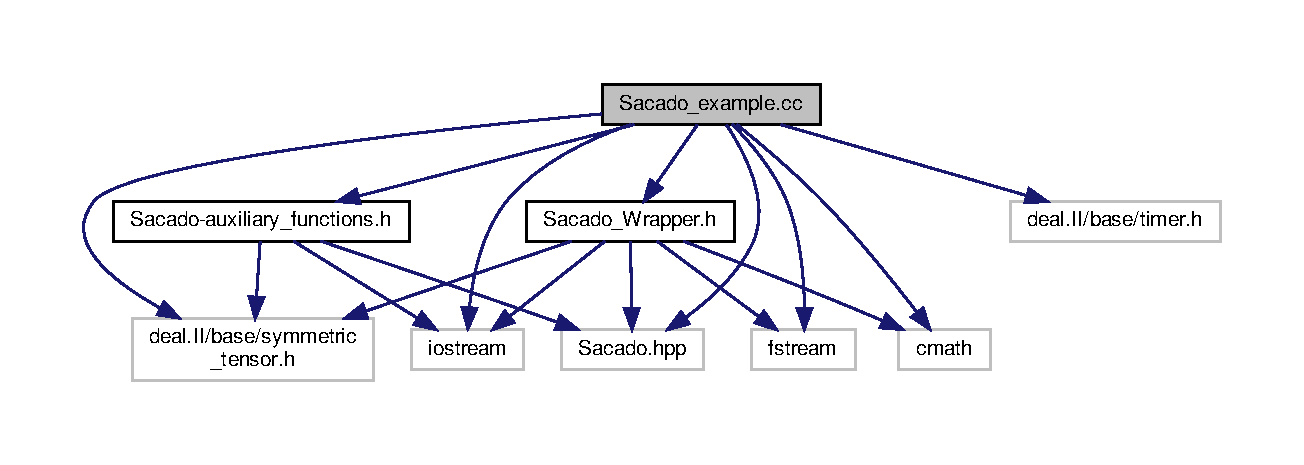
\includegraphics[width=350pt]{Sacado__example_8cc__incl}
\end{center}
\end{figure}
\subsection*{Typedefs}
\begin{DoxyCompactItemize}
\item 
using \hyperlink{Sacado__example_8cc_a868b94676739e612d9c95940e70892a9}{fad\+\_\+double} = Sacado\+::\+Fad\+::\+D\+Fad$<$ double $>$
\end{DoxyCompactItemize}
\subsection*{Functions}
\begin{DoxyCompactItemize}
\item 
void \hyperlink{Sacado__example_8cc_a71b2675e62203edc430e7ffc8a365193}{sacado\+\_\+test\+\_\+scalar} ()
\item 
void \hyperlink{Sacado__example_8cc_a8ef4ff1e9526ca8451cdcd1678366d2c}{sacado\+\_\+test\+\_\+2} ()
\item 
void \hyperlink{Sacado__example_8cc_ae45e1df0eec246dbb6f2c3d28a2a58e4}{sacado\+\_\+test\+\_\+3} ()
\item 
void \hyperlink{Sacado__example_8cc_ae63cc8526935cb0512668e83cfc7b929}{sacado\+\_\+test\+\_\+3B} ()
\item 
void \hyperlink{Sacado__example_8cc_a2f4def4563e31d720e07bc7d6363ebe2}{sacado\+\_\+test\+\_\+4} ()
\item 
void \hyperlink{Sacado__example_8cc_a327dbbb4ea7fc9840c46d149843a44c2}{sacado\+\_\+test\+\_\+5} ()
\item 
void \hyperlink{Sacado__example_8cc_a27450ab52a9d4250e3f5a5f2a3f8f317}{sacado\+\_\+test\+\_\+6} ()
\item 
void \hyperlink{Sacado__example_8cc_a0b694459e5e15c1578d97e637faba8de}{sacado\+\_\+test\+\_\+7} ()
\item 
void \hyperlink{Sacado__example_8cc_aa7108ff8393b98d66dfef50899d048d9}{sacado\+\_\+test\+\_\+8} ()
\item 
void \hyperlink{Sacado__example_8cc_ae176f83fe1943e102fe325d4a14f097e}{sacado\+\_\+test\+\_\+9} ()
\item 
void \hyperlink{Sacado__example_8cc_a70dbdff0078e09883ba02d2724a432b2}{sacado\+\_\+test\+\_\+10} ()
\item 
int \hyperlink{Sacado__example_8cc_ae66f6b31b5ad750f1fe042a706a4e3d4}{main} ()
\end{DoxyCompactItemize}


\subsection{Typedef Documentation}
\index{Sacado\+\_\+example.\+cc@{Sacado\+\_\+example.\+cc}!fad\+\_\+double@{fad\+\_\+double}}
\index{fad\+\_\+double@{fad\+\_\+double}!Sacado\+\_\+example.\+cc@{Sacado\+\_\+example.\+cc}}
\subsubsection[{\texorpdfstring{fad\+\_\+double}{fad_double}}]{\setlength{\rightskip}{0pt plus 5cm}using {\bf fad\+\_\+double} =  Sacado\+::\+Fad\+::\+D\+Fad$<$double$>$}\hypertarget{Sacado__example_8cc_a868b94676739e612d9c95940e70892a9}{}\label{Sacado__example_8cc_a868b94676739e612d9c95940e70892a9}


\subsection{Function Documentation}
\index{Sacado\+\_\+example.\+cc@{Sacado\+\_\+example.\+cc}!main@{main}}
\index{main@{main}!Sacado\+\_\+example.\+cc@{Sacado\+\_\+example.\+cc}}
\subsubsection[{\texorpdfstring{main()}{main()}}]{\setlength{\rightskip}{0pt plus 5cm}int main (
\begin{DoxyParamCaption}
{}
\end{DoxyParamCaption}
)}\hypertarget{Sacado__example_8cc_ae66f6b31b5ad750f1fe042a706a4e3d4}{}\label{Sacado__example_8cc_ae66f6b31b5ad750f1fe042a706a4e3d4}


References sacado\+\_\+test\+\_\+10(), sacado\+\_\+test\+\_\+2(), sacado\+\_\+test\+\_\+3(), sacado\+\_\+test\+\_\+3\+B(), sacado\+\_\+test\+\_\+4(), sacado\+\_\+test\+\_\+5(), sacado\+\_\+test\+\_\+6(), sacado\+\_\+test\+\_\+7(), sacado\+\_\+test\+\_\+8(), sacado\+\_\+test\+\_\+9(), and sacado\+\_\+test\+\_\+scalar().


\begin{DoxyCode}
1050 \{
1051     \hyperlink{Sacado__example_8cc_a71b2675e62203edc430e7ffc8a365193}{sacado\_test\_scalar} ();
1052 
1053     std::cout << std::endl;
1054 
1055     \hyperlink{Sacado__example_8cc_a8ef4ff1e9526ca8451cdcd1678366d2c}{sacado\_test\_2} ();
1056 
1057     std::cout << std::endl;
1058 
1059     \hyperlink{Sacado__example_8cc_ae45e1df0eec246dbb6f2c3d28a2a58e4}{sacado\_test\_3} ();
1060 
1061     std::cout << std::endl;
1062 
1063     \hyperlink{Sacado__example_8cc_ae63cc8526935cb0512668e83cfc7b929}{sacado\_test\_3B} ();
1064 
1065     std::cout << std::endl;
1066 
1067     \hyperlink{Sacado__example_8cc_a2f4def4563e31d720e07bc7d6363ebe2}{sacado\_test\_4}();
1068 
1069     std::cout << std::endl;
1070 
1071     \hyperlink{Sacado__example_8cc_a327dbbb4ea7fc9840c46d149843a44c2}{sacado\_test\_5}();
1072 
1073     std::cout << std::endl;
1074 
1075     \hyperlink{Sacado__example_8cc_a27450ab52a9d4250e3f5a5f2a3f8f317}{sacado\_test\_6}();
1076 
1077     std::cout << std::endl;
1078 
1079     \hyperlink{Sacado__example_8cc_a0b694459e5e15c1578d97e637faba8de}{sacado\_test\_7}();
1080 
1081     std::cout << std::endl;
1082 
1083     \hyperlink{Sacado__example_8cc_aa7108ff8393b98d66dfef50899d048d9}{sacado\_test\_8}();
1084 
1085     std::cout << std::endl;
1086 
1087     \hyperlink{Sacado__example_8cc_ae176f83fe1943e102fe325d4a14f097e}{sacado\_test\_9}();
1088 
1089     std::cout << std::endl;
1090 
1091     \hyperlink{Sacado__example_8cc_a70dbdff0078e09883ba02d2724a432b2}{sacado\_test\_10}();
1092 \}
\end{DoxyCode}
\index{Sacado\+\_\+example.\+cc@{Sacado\+\_\+example.\+cc}!sacado\+\_\+test\+\_\+10@{sacado\+\_\+test\+\_\+10}}
\index{sacado\+\_\+test\+\_\+10@{sacado\+\_\+test\+\_\+10}!Sacado\+\_\+example.\+cc@{Sacado\+\_\+example.\+cc}}
\subsubsection[{\texorpdfstring{sacado\+\_\+test\+\_\+10()}{sacado_test_10()}}]{\setlength{\rightskip}{0pt plus 5cm}void sacado\+\_\+test\+\_\+10 (
\begin{DoxyParamCaption}
{}
\end{DoxyParamCaption}
)}\hypertarget{Sacado__example_8cc_a70dbdff0078e09883ba02d2724a432b2}{}\label{Sacado__example_8cc_a70dbdff0078e09883ba02d2724a432b2}


References Sacado\+\_\+\+Wrapper\+::\+S\+W\+\_\+double2$<$ dim $>$\+::get\+\_\+curvature(), Sacado\+\_\+\+Wrapper\+::\+Do\+Fs\+\_\+summary$<$ dim $>$\+::get\+\_\+curvature(), Sacado\+\_\+\+Wrapper\+::\+S\+W\+\_\+double2$<$ dim $>$\+::get\+\_\+tangent(), and Sacado\+\_\+\+Wrapper\+::\+Do\+Fs\+\_\+summary$<$ dim $>$\+::init\+\_\+set\+\_\+dofs().



Referenced by main().


\begin{DoxyCode}
936 \{
937     \textcolor{keyword}{const} \textcolor{keywordtype}{unsigned} \textcolor{keywordtype}{int} dim=3;
938 
939     std::cout << \textcolor{stringliteral}{"Test 10:"} << std::endl;
940 
941     \textcolor{comment}{// Defining the inputs (material parameters, strain tensor)}
942      \textcolor{keywordtype}{double} lambda=1;
943      \textcolor{keywordtype}{double} mu=2;
944      SymmetricTensor<2,dim, double> eps;
945      \textcolor{keywordtype}{double} phi = 0.3;
946 
947      eps[0][0] = 1.;
948      eps[1][1] = 2.;
949      eps[2][2] = 3.;
950 
951      eps[0][1] = 4.;
952      eps[0][2] = 5.;
953      eps[1][2] = 6.;
954 
955     \textcolor{comment}{// Declaring the special data types containing all derivatives}
956      \textcolor{keyword}{typedef} Sacado::Fad::DFad<double> \hyperlink{Sacado__Wrapper_8h_a7e0893207b87dad05c66a34baac8ed2e}{DFadType};
957 
958     \textcolor{comment}{// Declare the variables \(\backslash\)a eps\_fad and \(\backslash\)a phi\_fad as the special Wrapper data types}
959      \hyperlink{classSacado__Wrapper_1_1SymTensor2}{Sacado\_Wrapper::SymTensor2<dim>} eps\_fad;
960      \hyperlink{classSacado__Wrapper_1_1SW__double2}{Sacado\_Wrapper::SW\_double2<dim>} phi\_fad;
961 
962     \textcolor{comment}{// Declare the summary data type relating all the dofs and initialising them too}
963      \hyperlink{classSacado__Wrapper_1_1DoFs__summary}{Sacado\_Wrapper::DoFs\_summary<dim>} DoFs\_summary;
964      DoFs\_summary.\hyperlink{classSacado__Wrapper_1_1DoFs__summary_ae273d0fa3197118a11d7005523e27d8a}{init\_set\_dofs}(eps\_fad, eps, phi\_fad, phi);
965 
966     \textcolor{comment}{// The variables are outputted to give some insight into the storage of the values (derivatives still
       trivial).}
967      std::cout << \textcolor{stringliteral}{"eps\_fad="} << eps\_fad << std::endl;
968      std::cout << \textcolor{stringliteral}{"phi\_fad="} << phi\_fad << std::endl;
969 
970     \textcolor{comment}{// Compute eps² = eps\_ij * eps\_jk in index notation}
971      SymmetricTensor<2,dim, Sacado::Fad::DFad<DFadType> > eps\_fad\_squared;
972      \textcolor{keywordflow}{for} ( \textcolor{keywordtype}{unsigned} \textcolor{keywordtype}{int} i=0; i<dim; ++i)
973         \textcolor{keywordflow}{for} ( \textcolor{keywordtype}{unsigned} \textcolor{keywordtype}{int} k=0; k<dim; ++k )
974             \textcolor{keywordflow}{for} ( \textcolor{keywordtype}{unsigned} \textcolor{keywordtype}{int} j=0; j<dim; ++j )
975                 \textcolor{keywordflow}{if} ( i>=k )
976                     eps\_fad\_squared[i][k] += eps\_fad[i][j] * eps\_fad[j][k];
977 
978     \textcolor{comment}{// Compute the strain energy density}
979      Sacado::Fad::DFad<DFadType> energy;
980      energy = lambda/2. * trace(eps\_fad)*trace(eps\_fad) + mu * trace(eps\_fad\_squared) + 25 * phi\_fad * 
      trace(eps\_fad);
981 
982     \textcolor{comment}{// The energy is outputted to give some insight into the storage of the values and derivatives. \(\backslash\)n}
983     \textcolor{comment}{// energy=399 [ 17.5 32 40 21.5 48 25.5 150 ] [ 17.5 [ 5 0 0 1 0 1 25 ] 32 [ 0 8 0 0 0 0 0 ] 40 [ 0 0 8
       0 0 0 0 ]}
984     \textcolor{comment}{// 21.5 [ 1 0 0 5 0 1 25 ] 48 [ 0 0 0 0 8 0 0 ] 25.5 [ 1 0 0 1 0 5 25 ] 150 [ 25 0 0 25 0 25 0 ] ]}
985 
986      std::cout << \textcolor{stringliteral}{"energy="} << energy << std::endl;
987 
988     \textcolor{comment}{// Compute sigma as \(\backslash\)f[ \(\backslash\)boldsymbol\{\(\backslash\)sigma\} = \(\backslash\)frac\{\(\backslash\)partial \(\backslash\)Psi\}\{\(\backslash\)partial \(\backslash\)boldsymbol\{\(\backslash\)varepsilon\}\}
       \(\backslash\)f]}
989      SymmetricTensor<2,dim> sigma\_Sac;
990      eps\_fad.get\_tangent(sigma\_Sac, energy);
991      std::cout << \textcolor{stringliteral}{"sigma\_Sacado="} << sigma\_Sac << std::endl;
992 
993      \textcolor{keywordtype}{double} d\_energy\_d\_phi;
994      phi\_fad.\hyperlink{classSacado__Wrapper_1_1SW__double2_ad51ba1e79171d60861b28098dfef903d}{get\_tangent}(d\_energy\_d\_phi, energy);
995      std::cout << \textcolor{stringliteral}{"d\_energy\_d\_phi="} << d\_energy\_d\_phi << std::endl;
996 
997 
998     \textcolor{comment}{// Analytical stress tensor:}
999      SymmetricTensor<2,dim> sigma;
1000      sigma = lambda*trace(eps)*unit\_symmetric\_tensor<dim>() + 2. * mu * eps;
1001      std::cout << \textcolor{stringliteral}{"analy. sigma="} << sigma << std::endl;
1002 
1003 
1004     \textcolor{comment}{// Sacado stress tangent (or eps curvature) as \(\backslash\)f[ \(\backslash\)frac\{\(\backslash\)partial^2 \(\backslash\)Psi\}\{\(\backslash\)partial
       \(\backslash\)boldsymbol\{\(\backslash\)varepsilon\}^2\} \(\backslash\)f]}
1005      SymmetricTensor<4,dim> C\_Sac;
1006      eps\_fad.get\_curvature(C\_Sac, energy);
1007 
1008     \textcolor{comment}{// Sacado phi curvature as \(\backslash\)f[ \(\backslash\)frac\{\(\backslash\)partial^2 \(\backslash\)Psi\}\{\(\backslash\)partial \(\backslash\)varphi^2\} \(\backslash\)f]}
1009      \textcolor{keywordtype}{double} d2\_energy\_d\_phi\_2;
1010      phi\_fad.\hyperlink{classSacado__Wrapper_1_1SW__double2_a7d3f3a21cd842645af9861bf50308825}{get\_curvature}(d2\_energy\_d\_phi\_2, energy);
1011      std::cout << \textcolor{stringliteral}{"d2\_energy\_d\_phi\_2="} << d2\_energy\_d\_phi\_2 << std::endl;
1012 
1013     \textcolor{comment}{// Sacado derivatives \(\backslash\)f[ \(\backslash\)frac\{\(\backslash\)partial^2 \(\backslash\)Psi\}\{\(\backslash\)partial \(\backslash\)boldsymbol\{\(\backslash\)varepsilon\} \(\backslash\)partial \(\backslash\)varphi\}
       \(\backslash\)f]}
1014      SymmetricTensor<2,dim> d2\_energy\_d\_eps\_d\_phi;
1015      DoFs\_summary.\hyperlink{classSacado__Wrapper_1_1DoFs__summary_adf29bfda10814ecee9572a4751d34db0}{get\_curvature}(d2\_energy\_d\_eps\_d\_phi, energy, eps\_fad, phi\_fad);
1016      std::cout << \textcolor{stringliteral}{"d2\_energy\_d\_eps\_d\_phi="} << d2\_energy\_d\_eps\_d\_phi << std::endl;
1017 
1018     \textcolor{comment}{// Sacado derivatives \(\backslash\)f[ \(\backslash\)frac\{\(\backslash\)partial^2 \(\backslash\)Psi\}\{\(\backslash\)partial \(\backslash\)varphi \(\backslash\)partial \(\backslash\)boldsymbol\{\(\backslash\)varepsilon\}\}
       \(\backslash\)f]}
1019      SymmetricTensor<2,dim> d2\_energy\_d\_phi\_d\_eps;
1020      DoFs\_summary.\hyperlink{classSacado__Wrapper_1_1DoFs__summary_adf29bfda10814ecee9572a4751d34db0}{get\_curvature}(d2\_energy\_d\_phi\_d\_eps, energy, phi\_fad, eps\_fad);
1021      std::cout << \textcolor{stringliteral}{"d2\_energy\_d\_phi\_d\_eps="} << d2\_energy\_d\_phi\_d\_eps << std::endl;
1022 
1023     \textcolor{comment}{// When you consider the output: \(\backslash\)n}
1024     \textcolor{comment}{// d2\_energy\_d\_eps\_d\_phi=25 0 0 0 25 0 0 0 25 \(\backslash\)n}
1025     \textcolor{comment}{// d2\_energy\_d\_phi\_d\_eps=25 0 0 0 25 0 0 0 25 \(\backslash\)n}
1026     \textcolor{comment}{// in detail you will notice that both second derivatives are identical. This compplies with the
       Schwarz integrability condition (Symmetry of second derivatives)}
1027     \textcolor{comment}{// (ignoring all limitation and requirements), it holds}
1028     \textcolor{comment}{// \(\backslash\)f[ \(\backslash\)frac\{\(\backslash\)partial^2 \(\backslash\)Psi\}\{\(\backslash\)partial \(\backslash\)boldsymbol\{\(\backslash\)varepsilon\} \(\backslash\)partial \(\backslash\)varphi\} = \(\backslash\)frac\{\(\backslash\)partial^2
       \(\backslash\)Psi\}\{\(\backslash\)partial \(\backslash\)varphi \(\backslash\)partial \(\backslash\)boldsymbol\{\(\backslash\)varepsilon\}\}  \(\backslash\)f]}
1029 
1030     \textcolor{comment}{// Analytical stress tangent}
1031      SymmetricTensor<4,dim> C\_analy;
1032      C\_analy = lambda * outer\_product(unit\_symmetric\_tensor<dim>(), unit\_symmetric\_tensor<dim>()) + 2. * mu
       * identity\_tensor<dim>();
1033 
1034     \textcolor{comment}{// Compute the error for the stress tangent}
1035      \textcolor{keywordtype}{double} error\_Sacado\_vs\_analy=0;
1036      \textcolor{keywordflow}{for} (\textcolor{keywordtype}{unsigned} \textcolor{keywordtype}{int} i=0; i<dim; ++i)
1037         \textcolor{keywordflow}{for} ( \textcolor{keywordtype}{unsigned} \textcolor{keywordtype}{int} j=0; j<dim; ++j)
1038             \textcolor{keywordflow}{for} ( \textcolor{keywordtype}{unsigned} \textcolor{keywordtype}{int} k=0; k<dim; ++k)
1039                 \textcolor{keywordflow}{for} ( \textcolor{keywordtype}{unsigned} \textcolor{keywordtype}{int} l=0; l<dim; ++l)
1040                     error\_Sacado\_vs\_analy += std::fabs(C\_Sac[i][j][k][l] - C\_analy[i][j][k][l]);
1041      std::cout << \textcolor{stringliteral}{"Numerical error="} << error\_Sacado\_vs\_analy << std::endl;
1042 \}
\end{DoxyCode}
\index{Sacado\+\_\+example.\+cc@{Sacado\+\_\+example.\+cc}!sacado\+\_\+test\+\_\+2@{sacado\+\_\+test\+\_\+2}}
\index{sacado\+\_\+test\+\_\+2@{sacado\+\_\+test\+\_\+2}!Sacado\+\_\+example.\+cc@{Sacado\+\_\+example.\+cc}}
\subsubsection[{\texorpdfstring{sacado\+\_\+test\+\_\+2()}{sacado_test_2()}}]{\setlength{\rightskip}{0pt plus 5cm}void sacado\+\_\+test\+\_\+2 (
\begin{DoxyParamCaption}
{}
\end{DoxyParamCaption}
)}\hypertarget{Sacado__example_8cc_a8ef4ff1e9526ca8451cdcd1678366d2c}{}\label{Sacado__example_8cc_a8ef4ff1e9526ca8451cdcd1678366d2c}


Referenced by main().


\begin{DoxyCode}
67 \{
68     std::cout << \textcolor{stringliteral}{"Test 2:"} << std::endl;
69 
70     \textcolor{comment}{// First we set the dimension \(\backslash\)a dim: 2D->dim=2; 3D->dim=3 \(\backslash\)n This defines the "size" of the tensors
       and the number of dofs. Ex2 only works in 3D, whereas the following Ex3 is set up dimension-independent.}
71     \textcolor{keyword}{const} \textcolor{keywordtype}{unsigned} \textcolor{keywordtype}{int} dim = 3;
72 
73     \textcolor{comment}{// Declare our input, auxiliary and output variables as SymmetricTensors consisting of fad\_doubles
       (instead of the standard SymmetricTensor out of doubles)}
74     SymmetricTensor<2,dim, fad\_double> sigma, eps;
75 
76     \textcolor{comment}{// Init the strain tensor (the point at which the derivative shall be computed)}
77     eps[0][0] = 1;
78     eps[1][1] = 2;
79     eps[2][2] = 3;
80     eps[0][1] = 4;
81     eps[0][2] = 5;
82     eps[1][2] = 6;
83 
84     \textcolor{comment}{// Now we declare the dofs. The derivative to a tensor requires all components, therefore we set the
       components of the strain tensor here one by one as the dofs.}
85     \textcolor{comment}{// Because our tensors are symmetric, we only need 6 components in 3D instead of 9 for a full second
       order tensor}
86     eps[0][0].diff(0,6);
87     eps[1][1].diff(1,6);
88     eps[2][2].diff(2,6);
89     eps[0][1].diff(3,6);
90     eps[0][2].diff(4,6);
91     eps[1][2].diff(5,6);
92 
93     \textcolor{comment}{// The equation describing the stresses (here just a simple test case)}
94     sigma = eps;
95 
96     \textcolor{comment}{// Let's output the computed stress tensor.}
97     std::cout << sigma << std::endl;
98     \textcolor{comment}{// The resulting values of \(\backslash\)a sigma are fairly boring, due to our simple equation. It is the additional
       output generated by}
99     \textcolor{comment}{// this, that is interesting here: \(\backslash\)n}
100     \textcolor{comment}{// output: \(\backslash\)n}
101     \textcolor{comment}{// 1 [ 1 0 0 0 0 0 ] 4 [ 0 0 0 1 0 0 ] 5 [ 0 0 0 0 1 0 ] 4 [ 0 0 0 1 0 0 ] 2 [ 0 1 0 0 0 0 ] 6 [ 0 0 0
       0 0 1 ] 5 [ 0 0 0 0 1 0 ] 6 [ 0 0 0 0 0 1 ] 3 [ 0 0 1 0 0 0 ] \(\backslash\)n}
102     \textcolor{comment}{// The numbers 1, 4, 5, 4, ... are the entries in the stress tensor \(\backslash\)a sigma. In square brackets we see
       the derivatives of sigma with respect to all the dofs set previously}
103     \textcolor{comment}{// given in the order we defined them above. Meaning: The first entry in the square brackets
       corresponds to the 0-th dof set by}
104     \textcolor{comment}{// @code eps[0][0].diff(0,6); @endcode referring to the component (0,0) in the strain tensor \(\backslash\)a eps.}
105 
106     \textcolor{comment}{// Computing the derivatives for certain components of the resulting tangent modulus: \(\backslash\)n}
107     \textcolor{comment}{// We now access these lists of derivatives (output above in square brackets) for one component of the
       stress tensor \(\backslash\)a sigma at a time.}
108     \{
109         \textcolor{comment}{// Access the derivatives corresponding to the component (0,0) of the stress tensor \(\backslash\)a sigma}
110         \textcolor{keywordtype}{double} *derivs = &sigma[0][0].fastAccessDx(0);
111         \textcolor{comment}{// The following output will show us the same derivatives that we already saw above, just formatted
       differently \(\backslash\)n}
112         \textcolor{comment}{// output: d\_sigma[0][0]/d\_eps = 1 , 0 , 0 , 0 , 0 , 0 ,}
113         std::cout << \textcolor{stringliteral}{"d\_sigma[0][0]/d\_eps = "};
114         \textcolor{keywordflow}{for} ( \textcolor{keywordtype}{unsigned} \textcolor{keywordtype}{int} i=0; i<6; ++i)
115             std::cout << derivs[i] << \textcolor{stringliteral}{" , "};
116         std::cout << std::endl;
117     \}
118     \{
119         \textcolor{comment}{// Access the derivatives corresponding to the component (1,2) of the stress tensor \(\backslash\)a sigma}
120         \textcolor{keywordtype}{double} *derivs = &sigma[1][2].fastAccessDx(0);
121         \textcolor{comment}{// output: d\_sigma[1][2]/d\_eps = 0 , 0 , 0 , 0 , 0 , 1 ,}
122         std::cout << \textcolor{stringliteral}{"d\_sigma[1][2]/d\_eps = "};
123         \textcolor{keywordflow}{for} ( \textcolor{keywordtype}{unsigned} \textcolor{keywordtype}{int} i=0; i<6; ++i)
124             std::cout << derivs[i] << \textcolor{stringliteral}{" , "};
125         std::cout << std::endl;
126     \}
127 \}
\end{DoxyCode}
\index{Sacado\+\_\+example.\+cc@{Sacado\+\_\+example.\+cc}!sacado\+\_\+test\+\_\+3@{sacado\+\_\+test\+\_\+3}}
\index{sacado\+\_\+test\+\_\+3@{sacado\+\_\+test\+\_\+3}!Sacado\+\_\+example.\+cc@{Sacado\+\_\+example.\+cc}}
\subsubsection[{\texorpdfstring{sacado\+\_\+test\+\_\+3()}{sacado_test_3()}}]{\setlength{\rightskip}{0pt plus 5cm}void sacado\+\_\+test\+\_\+3 (
\begin{DoxyParamCaption}
{}
\end{DoxyParamCaption}
)}\hypertarget{Sacado__example_8cc_ae45e1df0eec246dbb6f2c3d28a2a58e4}{}\label{Sacado__example_8cc_ae45e1df0eec246dbb6f2c3d28a2a58e4}


Referenced by main().


\begin{DoxyCode}
132 \{
133     std::cout << \textcolor{stringliteral}{"Test 3:"} << std::endl;
134 
135     \textcolor{keyword}{const} \textcolor{keywordtype}{unsigned} \textcolor{keywordtype}{int} dim = 3;
136 
137     \textcolor{comment}{// Here we also define some constant, for instance the bulk modulus \(\backslash\)a kappa and the second Lamè
       parameter \(\backslash\)a mu.}
138     \textcolor{comment}{// We now also define one of our constants as fad\_double. By doing this we can use the normal
       multiplication (see below).}
139     \textcolor{keywordtype}{double} kappa\_param = 5;
140     \hyperlink{Sacado__example_8cc_a868b94676739e612d9c95940e70892a9}{fad\_double} kappa (kappa\_param);
141     \textcolor{comment}{// The second constant remains as a double just to show the difference.}
142     \textcolor{keywordtype}{double} mu = 2;
143 
144     SymmetricTensor<2,dim, fad\_double> sigma, eps;
145 
146     \textcolor{comment}{// To simplify the access to the dofs we define a map that relate the components of our strain tensor
       to the dof-nbr}
147     std::map<unsigned int,std::pair<unsigned int,unsigned int>> std\_map\_indicies;
148 
149     \textcolor{comment}{// The point at which the derivative shall be computed: \(\backslash\)n}
150     \textcolor{comment}{// As mentioned previously, we will implement this example for 2D and 3D, hence we once have to set up
       a strain tensor}
151     \textcolor{comment}{// and the derivatives for 3D with 6 independent components ...}
152     \textcolor{keywordflow}{if}(dim==3)
153     \{
154         eps[0][0] = 1;
155         eps[1][1] = 2;
156         eps[2][2] = 3;
157         
158         eps[0][1] = 4;
159         eps[0][2] = 5;
160         eps[1][2] = 6;
161         
162         
163         eps[0][0].diff(0,6);
164         eps[0][1].diff(1,6);
165         eps[0][2].diff(2,6);
166         eps[1][1].diff(3,6);
167         eps[1][2].diff(4,6);
168         eps[2][2].diff(5,6);
169         
170         \textcolor{comment}{// By using the map and the following pairs, we have to set up the relation between strain
       components and dofs only once}
171         \textcolor{comment}{// and can use the map to access the entries of the list later, without possibly mixing up indices
       and creating errors.}
172         \textcolor{comment}{// Please don't be confused, but the dofs in the Wrapper are set up}
173         \textcolor{comment}{// in a different order that we showed earlier. Earlier: (0,0)-(1,1)-(2,2)-...; Now:
       (0,0)-(0,1)-(0,2)-...}
174         std::pair<unsigned int, unsigned int> tmp\_pair;
175         tmp\_pair.first=0; tmp\_pair.second=0;
176         std\_map\_indicies[0] = tmp\_pair;
177 
178         tmp\_pair.first=0; tmp\_pair.second=1;
179         std\_map\_indicies[1] = tmp\_pair;
180 
181         tmp\_pair.first=0; tmp\_pair.second=2;
182         std\_map\_indicies[2] = tmp\_pair;
183 
184         tmp\_pair.first=1; tmp\_pair.second=1;
185         std\_map\_indicies[3] = tmp\_pair;
186 
187         tmp\_pair.first=1; tmp\_pair.second=2;
188         std\_map\_indicies[4] = tmp\_pair;
189 
190         tmp\_pair.first=2; tmp\_pair.second=2;
191         std\_map\_indicies[5] = tmp\_pair;
192     \}
193     \textcolor{comment}{// ... and once for 2D with just 3 independent components.}
194     \textcolor{keywordflow}{else} \textcolor{keywordflow}{if}(dim==2)
195     \{
196         eps[0][0] = 1;
197         eps[1][1] = 2;
198         
199         eps[0][1] = 4;
200 
201                 
202         eps[0][0].diff(0,3);
203         eps[0][1].diff(1,3);
204         eps[1][1].diff(2,3);
205         
206         std::pair<unsigned int, unsigned int> tmp\_pair;
207         tmp\_pair.first=0; tmp\_pair.second=0;
208         std\_map\_indicies[0] = tmp\_pair;
209         
210         tmp\_pair.first=0; tmp\_pair.second=1;
211         std\_map\_indicies[1] = tmp\_pair;
212         
213         tmp\_pair.first=1; tmp\_pair.second=1;
214         std\_map\_indicies[2] = tmp\_pair;        
215     \}
216     \textcolor{keywordflow}{else}
217     \{
218         \textcolor{keywordflow}{throw} std::runtime\_error(\textcolor{stringliteral}{"only dim==2 or dim==3 allowed"});
219     \}
220 
221     \textcolor{comment}{// Instead of calling the *.diff(*) on the components one-by-one we could also use the following
       for-loop, so}
222     \textcolor{comment}{// we also use the map to set the dofs (as we will do in the Wrapper later).}
223     \textcolor{comment}{// @code}
224     \textcolor{comment}{// for ( unsigned int x=0; x<((dim==2)?3:6); ++x )}
225     \textcolor{comment}{// \{}
226     \textcolor{comment}{//  unsigned int i=std\_map\_indicies[x].first;}
227     \textcolor{comment}{//  unsigned int j=std\_map\_indicies[x].second;}
228     \textcolor{comment}{//  eps[i][j].diff(x,((dim==2)?3:6));}
229     \textcolor{comment}{// \}}
230     \textcolor{comment}{// @endcode}
231 
232     \textcolor{comment}{// For our slightly more complicated stress equation we need the unit and deviatoric tensors.}
233     \textcolor{comment}{// We can simply define them by writing the values of the already existing deal.ii functions into newly}
234     \textcolor{comment}{// defined SymmetricTensors build from fad\_doubles.}
235     SymmetricTensor<2,dim, fad\_double> stdTensor\_I (( unit\_symmetric\_tensor<dim,fad\_double>()) );
236     SymmetricTensor<4,dim, fad\_double> stdTensor\_Idev ( (deviator\_tensor<dim,fad\_double>()) );
237     
238     \textcolor{comment}{// With everything set and defined, we can compute our stress \(\backslash\)a sigma according to:}
239     \textcolor{comment}{// \(\backslash\)f[ \(\backslash\)sigma = \(\backslash\)kappa \(\backslash\)cdot trace(\(\backslash\)varepsilon) \(\backslash\)cdot \(\backslash\)boldsymbol\{I\} + 2 \(\backslash\)cdot \(\backslash\)mu \(\backslash\)cdot
       \(\backslash\)varepsilon^\{dev\} \(\backslash\)f]}
240     \textcolor{comment}{// Here you can see that we can directly multiply the constant and the tensors when kappa is also
       declared as fad\_double}
241     sigma = kappa * (trace(eps) *  stdTensor\_I);
242     \textcolor{comment}{// We didn't do the same for mu to once again emphasize the difference between constants as double and
       as fad\_double. \(\backslash\)n}
243     \textcolor{comment}{// The remaining code uses a normal double constant.}
244     SymmetricTensor<2,dim,fad\_double> tmp = deviator<dim,fad\_double>(symmetrize<dim,fad\_double>(eps)); tmp*
      =(mu*2);
245     sigma +=  tmp;
246     \textcolor{comment}{// The fairly cumbersome computation is caused by the way the operators are set up for tensors out of
       fad\_doubles.}
247     
248     std::cout << \textcolor{stringliteral}{"sigma="} << sigma << std::endl;
249 
250     \textcolor{comment}{// Now we want to actually build our tangent modulus called \(\backslash\)a C\_Sacado that contains all the
       derivatives and relates}
251     \textcolor{comment}{// the stress tensor with the strain tensor. \(\backslash\)n}
252     \textcolor{comment}{// The fourth-order tensor \(\backslash\)a C\_Sacado is our final goal, we don't have to compute anything that is
       related to Sacado with}
253     \textcolor{comment}{// this tensor, so we can finally return to our standard SymmetricTensor out of doubles. The latter is
       necessary to use}
254     \textcolor{comment}{// the tangent in the actual FE code.}
255     SymmetricTensor<4,dim> C\_Sacado;
256 
257     \textcolor{comment}{// As in Ex2 we access the components of the stress tensor one by one. In order to capture all of them
       we sum over the}
258     \textcolor{comment}{// components i and j of the stress tensor.}
259     \textcolor{keywordflow}{for} ( \textcolor{keywordtype}{unsigned} \textcolor{keywordtype}{int} i=0; i<dim; ++i)
260         \textcolor{keywordflow}{for} ( \textcolor{keywordtype}{unsigned} \textcolor{keywordtype}{int} j=0; j<dim; ++j )
261         \{
262             \textcolor{keywordtype}{double} *derivs = &sigma[i][j].fastAccessDx(0); \textcolor{comment}{// Access the derivatives of the (i,j)-th
       component of \(\backslash\)a sigma}
263 
264             \textcolor{comment}{// To visually ensure that every stress component has in fact all 6 derivatives for 3D or 3 for
       2D, we output the size:}
265             std::cout<<\textcolor{stringliteral}{"size: "}<<sigma[i][j].size()<<std::endl;
266 
267             \textcolor{comment}{// We loop over all the dofs. To be able to use this independent of the chosen dimension \(\backslash\)a
       dim, we use a ternary operator}
268             \textcolor{comment}{// to decide whether we have to loop over 6 derivatives or just 3.}
269             \textcolor{keywordflow}{for}(\textcolor{keywordtype}{unsigned} \textcolor{keywordtype}{int} x=0;x<((dim==2)?3:6);++x)
270             \{
271                 \textcolor{keywordtype}{unsigned} \textcolor{keywordtype}{int} k=std\_map\_indicies[x].first;
272                 \textcolor{keywordtype}{unsigned} \textcolor{keywordtype}{int} l=std\_map\_indicies[x].second;
273 
274                 \textcolor{keywordflow}{if}(k!=l)\textcolor{comment}{/*Compare to Voigt notation since only SymmetricTensor instead of Tensor*/}
275                 \{
276                     C\_Sacado[i][j][k][l] = 0.5*derivs[x];
277                     C\_Sacado[i][j][l][k] = 0.5*derivs[x];
278                 \}
279                 \textcolor{keywordflow}{else}
280                     C\_Sacado[i][j][k][l] = derivs[x];
281             \}            
282             
283         \}
284 
285     \textcolor{comment}{// After resembling the fourth-order tensor, we now have got our tangent saved in \(\backslash\)a C\_Sacado ready to
       be used}
286 
287     \textcolor{comment}{// To ensure that Sacado works properly, we can compute the analytical tangent for comparison}
288     \textcolor{keywordtype}{double} kappa\_d = 5;
289     \textcolor{keywordtype}{double} mu\_d = 2;
290     \textcolor{comment}{// Our stress equation in this example is still simple enough to derive the tangent analytically by
       hand:}
291     \textcolor{comment}{// \(\backslash\)f[ \(\backslash\)overset\{4\}\{C\_\{analy\}\} = \(\backslash\)kappa \(\backslash\)cdot \(\backslash\)boldsymbol\{I\} \(\backslash\)otimes \(\backslash\)boldsymbol\{I\} + 2 \(\backslash\)cdot \(\backslash\)mu \(\backslash\)cdot
       \(\backslash\)overset\{4\}\{I^\{dev\}\} \(\backslash\)f]}
292     SymmetricTensor<4,dim> C\_analy = kappa\_d * outer\_product(unit\_symmetric\_tensor<dim>(), 
      unit\_symmetric\_tensor<dim>()) + 2* mu\_d * deviator\_tensor<dim>();
293 
294 
295     \textcolor{comment}{// We again define our strain tensor \(\backslash\)a eps\_d (*\_d for standard double in contrast to fad\_double)}
296     SymmetricTensor<2,dim> eps\_d;
297     
298     \textcolor{keywordflow}{if}(dim==3)
299     \{
300         eps\_d[0][0] = 1;
301         eps\_d[1][1] = 2;
302         eps\_d[2][2] = 3;
303         
304         eps\_d[0][1] = 4;
305         eps\_d[0][2] = 5;
306         eps\_d[2][1] = 6;
307 
308     \}
309     \textcolor{keywordflow}{else} \textcolor{keywordflow}{if}(dim==2)
310     \{
311         eps\_d[0][0] = 1;
312         eps\_d[1][1] = 2;
313         
314         eps\_d[1][0] = 4;
315         
316     \}
317     \textcolor{keywordflow}{else}
318     \{
319         \textcolor{keywordflow}{throw} std::runtime\_error(\textcolor{stringliteral}{"only dim==2 or dim==3 allowed"});
320     \}
321     \textcolor{comment}{// @todo use boldsymbol for tensors}
322     \textcolor{comment}{//}
323     \textcolor{comment}{// To output the stress tensor we first have to compute it. We do this here via}
324     \textcolor{comment}{// \(\backslash\)f[ \(\backslash\)sigma = \(\backslash\)overset\{4\}\{C\_\{analy\}\} : \(\backslash\)varepsilon \(\backslash\)f]}
325     \textcolor{comment}{// The output exactly matched the result obtained with Sacado.}
326     \textcolor{comment}{// @note Checking the Sacado stress tensor against an analytically computed or otherwise determined
       stress tensor is absolutely no way to check whether}
327     \textcolor{comment}{// the tangent computed via Sacado is correct. When we compute the stress tensor with Sacado and for
       example mix up a + and - sign, this might not matter}
328     \textcolor{comment}{// at all if the number that is added or subtracted is small. However, for the tangent this nasty sign
       can be very critical. Just keep in mind: the}
329     \textcolor{comment}{// tangent has 81 components and the stress tensor just 9, so how does one want to verify 81 variables
       by comparing 9?}
330     \textcolor{comment}{//}
331     std::cout << \textcolor{stringliteral}{"sigma\_analy: "} << (C\_analy*eps\_d) << std::endl;
332     
333     \textcolor{comment}{// That's the reason we compare all the entries in the Sacado and the analytical tensor one by one}
334     \textcolor{keywordflow}{for} (\textcolor{keywordtype}{unsigned} \textcolor{keywordtype}{int} i=0; i<dim; ++i)
335         \textcolor{keywordflow}{for} ( \textcolor{keywordtype}{unsigned} \textcolor{keywordtype}{int} j=0; j<dim; ++j)
336             \textcolor{keywordflow}{for} ( \textcolor{keywordtype}{unsigned} \textcolor{keywordtype}{int} k=0; k<dim; ++k)
337                 \textcolor{keywordflow}{for} ( \textcolor{keywordtype}{unsigned} \textcolor{keywordtype}{int} l=0; l<dim; ++l)
338                     std::cout << \textcolor{stringliteral}{"C\_analy["}<<i<<\textcolor{stringliteral}{"]["}<<j<<\textcolor{stringliteral}{"]["}<<k<<\textcolor{stringliteral}{"]["}<<l<<\textcolor{stringliteral}{"] = "} << C\_analy[i][j][k][l] <<
       \textcolor{stringliteral}{" vs C\_Sacado: "} << C\_Sacado[i][j][k][l] << std::endl;
339 
340 
341     \textcolor{comment}{// To simplify the comparison we compute a scalar error as the sum of the absolute differences of each
       component}
342     \textcolor{keywordtype}{double} error\_Sacado\_vs\_analy=0;
343     \textcolor{keywordflow}{for} (\textcolor{keywordtype}{unsigned} \textcolor{keywordtype}{int} i=0; i<dim; ++i)
344         \textcolor{keywordflow}{for} ( \textcolor{keywordtype}{unsigned} \textcolor{keywordtype}{int} j=0; j<dim; ++j)
345             \textcolor{keywordflow}{for} ( \textcolor{keywordtype}{unsigned} \textcolor{keywordtype}{int} k=0; k<dim; ++k)
346                 \textcolor{keywordflow}{for} ( \textcolor{keywordtype}{unsigned} \textcolor{keywordtype}{int} l=0; l<dim; ++l)
347                     error\_Sacado\_vs\_analy += std::fabs(C\_Sacado[i][j][k][l] - C\_analy[i][j][k][l]);
348                     
349 
350     \textcolor{comment}{// As desired: The numerical error is zero (0 in double precision) and the tensor components are equal}
351     std::cout << \textcolor{stringliteral}{"numerical error: "} << error\_Sacado\_vs\_analy << std::endl;
352 \}
\end{DoxyCode}
\index{Sacado\+\_\+example.\+cc@{Sacado\+\_\+example.\+cc}!sacado\+\_\+test\+\_\+3B@{sacado\+\_\+test\+\_\+3B}}
\index{sacado\+\_\+test\+\_\+3B@{sacado\+\_\+test\+\_\+3B}!Sacado\+\_\+example.\+cc@{Sacado\+\_\+example.\+cc}}
\subsubsection[{\texorpdfstring{sacado\+\_\+test\+\_\+3\+B()}{sacado_test_3B()}}]{\setlength{\rightskip}{0pt plus 5cm}void sacado\+\_\+test\+\_\+3B (
\begin{DoxyParamCaption}
{}
\end{DoxyParamCaption}
)}\hypertarget{Sacado__example_8cc_ae63cc8526935cb0512668e83cfc7b929}{}\label{Sacado__example_8cc_ae63cc8526935cb0512668e83cfc7b929}


References Sacado\+\_\+\+Wrapper\+::\+Sym\+Tensor$<$ dim $>$\+::get\+\_\+tangent(), Sacado\+\_\+\+Wrapper\+::\+Sym\+Tensor$<$ dim $>$\+::init(), and Sacado\+\_\+\+Wrapper\+::\+Sym\+Tensor$<$ dim $>$\+::set\+\_\+dofs().



Referenced by main().


\begin{DoxyCode}
357 \{
358     std::cout << \textcolor{stringliteral}{"Test 3B:"} << std::endl;
359     \textcolor{keyword}{const} \textcolor{keywordtype}{unsigned} \textcolor{keywordtype}{int} dim=3;
360 
361     \textcolor{comment}{// The following declarations are usually input arguments. So you receive the strain tensor and the
       constants out of doubles.}
362     SymmetricTensor<2,dim> eps\_d;
363     eps\_d[0][0] = 1;
364     eps\_d[1][1] = 2;
365     eps\_d[2][2] = 3;
366 
367     eps\_d[0][1] = 4;
368     eps\_d[0][2] = 5;
369     eps\_d[1][2] = 6;
370 
371     \textcolor{keywordtype}{double} kappa = 5;
372     \textcolor{keywordtype}{double} mu = 2;
373 
374     \textcolor{comment}{// Now we start working with Sacado: \(\backslash\)n}
375     \textcolor{comment}{// When we use the index notation to compute e.g. our stress we do not need to declare our constants
       (here kappa, mu) as}
376     \textcolor{comment}{// fad\_double.}
377 
378     \textcolor{comment}{// We declare our strain tensor as the special data type Sacado\_Wrapper::SymTensor from the file
       "Sacado\_Wrapper.h"}
379     \textcolor{comment}{// where this data type was derived from the SymmetricTensor<2,dim,fad\_double>.}
380      \hyperlink{classSacado__Wrapper_1_1SymTensor}{Sacado\_Wrapper::SymTensor<dim>} eps;
381 
382     \textcolor{comment}{// Next we initialize our Sacado strain tensor with the values of the inputed double strain tensor:}
383      eps.\hyperlink{classSacado__Wrapper_1_1SymTensor_acbad579d5ead9e96ff46aa15d9b5aef4}{init}(eps\_d);
384 
385     \textcolor{comment}{// We define all the entries in the symmetric tensor \(\backslash\)a eps as the dofs. So we can later derive any
       variable}
386     \textcolor{comment}{// with respect to the strain tensor \(\backslash\)a eps.}
387      eps.\hyperlink{classSacado__Wrapper_1_1SymTensor_aa9e0fcc9d4e0a4120bedb8ef9b8d7ecb}{set\_dofs}();
388 
389     \textcolor{comment}{// Now we declare our output and auxiliary variables as Sacado-Tensors.}
390      SymmetricTensor<2,dim,fad\_double> sigma;
391 
392      SymmetricTensor<2,dim, fad\_double> stdTensor\_I (( unit\_symmetric\_tensor<dim,fad\_double>()) );
393 
394      \textcolor{comment}{// Our stress equation is now computed in index notation to simplify the use of the constants and}
395      \textcolor{comment}{// especially the use of the \(\backslash\)a deviator.}
396       \textcolor{keywordflow}{for} ( \textcolor{keywordtype}{unsigned} \textcolor{keywordtype}{int} i=0; i<dim; ++i)
397         \textcolor{keywordflow}{for} ( \textcolor{keywordtype}{unsigned} \textcolor{keywordtype}{int} j=0; j<dim; ++j )
398             sigma[i][j] = kappa * trace(eps) *  stdTensor\_I[i][j] + 2. * mu * deviator(eps)[i][j];
399 
400     \textcolor{comment}{// Finally we declare our desired tangent as the fourth order tensor \(\backslash\)a C\_Sacado and compute the
       tangent via}
401     \textcolor{comment}{// the command \(\backslash\)a get\_tangent.}
402      SymmetricTensor<4,dim> C\_Sacado;
403      eps.\hyperlink{classSacado__Wrapper_1_1SymTensor_ab97427c3b5cab279e58607cf431ab262}{get\_tangent}(C\_Sacado, sigma);
404 
405     \textcolor{comment}{// We could again compare the herein computed tangent with the analytical tangent from Ex2, but as
       before}
406     \textcolor{comment}{// the results are fairly boring, because Sacado hits the analytical tangent exactly --- no surprise
       for such}
407     \textcolor{comment}{// simple equations.}
408 
409     \textcolor{comment}{// And that's it. By using the Sacado\_wrapper we can achieve everything from Ex2 (besides the
       equations)}
410     \textcolor{comment}{// with just four lines of code namely:}
411     \textcolor{comment}{// - eps.init(eps\_d);    // To initialize the Sacado strain tensor}
412     \textcolor{comment}{// - eps.set\_dofs();     // To declare the components of eps as the dofs}
413     \textcolor{comment}{// - eps.get\_tangent(*); // To get the tangent}
414 \}
\end{DoxyCode}
\index{Sacado\+\_\+example.\+cc@{Sacado\+\_\+example.\+cc}!sacado\+\_\+test\+\_\+4@{sacado\+\_\+test\+\_\+4}}
\index{sacado\+\_\+test\+\_\+4@{sacado\+\_\+test\+\_\+4}!Sacado\+\_\+example.\+cc@{Sacado\+\_\+example.\+cc}}
\subsubsection[{\texorpdfstring{sacado\+\_\+test\+\_\+4()}{sacado_test_4()}}]{\setlength{\rightskip}{0pt plus 5cm}void sacado\+\_\+test\+\_\+4 (
\begin{DoxyParamCaption}
{}
\end{DoxyParamCaption}
)}\hypertarget{Sacado__example_8cc_a2f4def4563e31d720e07bc7d6363ebe2}{}\label{Sacado__example_8cc_a2f4def4563e31d720e07bc7d6363ebe2}


References Sacado\+\_\+\+Wrapper\+::\+Sym\+Tensor$<$ dim $>$\+::get\+\_\+tangent(), Sacado\+\_\+\+Wrapper\+::\+S\+W\+\_\+double$<$ dim $>$\+::get\+\_\+tangent(), Sacado\+\_\+\+Wrapper\+::\+Sym\+Tensor$<$ dim $>$\+::init(), Sacado\+\_\+\+Wrapper\+::\+S\+W\+\_\+double$<$ dim $>$\+::init(), and Sacado\+\_\+\+Wrapper\+::\+Do\+Fs\+\_\+summary$<$ dim $>$\+::set\+\_\+dofs().



Referenced by main().


\begin{DoxyCode}
419 \{
420     std::cout << \textcolor{stringliteral}{"Test 4:"} << std::endl;
421     \textcolor{keyword}{const} \textcolor{keywordtype}{unsigned} \textcolor{keywordtype}{int} dim=3;
422 
423     \textcolor{comment}{// The following declarations are usually input arguments. So you receive the strain tensor \(\backslash\)q eps\_d,}
424     \textcolor{comment}{// the damage variable \(\backslash\)a phi and the constants \(\backslash\)a kappa and \(\backslash\)a mu out of doubles.}
425     SymmetricTensor<2,dim> eps\_d;
426     eps\_d[0][0] = 1;
427     eps\_d[1][1] = 2;
428     eps\_d[2][2] = 3;
429 
430     eps\_d[0][1] = 4;
431     eps\_d[0][2] = 5;
432     eps\_d[1][2] = 6;
433 
434     \textcolor{keywordtype}{double} phi\_d = 0.3;
435 
436     \textcolor{comment}{// We don't need these constants in the current example.}
437     \textcolor{comment}{// double kappa = 5;}
438     \textcolor{comment}{// double mu = 2;}
439 
440 
441     \textcolor{comment}{// We set up our strain tensor as in Ex3B.}
442      \hyperlink{classSacado__Wrapper_1_1SymTensor}{Sacado\_Wrapper::SymTensor<dim>} eps;
443      \hyperlink{classSacado__Wrapper_1_1SW__double}{Sacado\_Wrapper::SW\_double<dim>} phi;
444 
445     \textcolor{comment}{// Initialize the strain tensor and the damage variable}
446      eps.\hyperlink{classSacado__Wrapper_1_1SymTensor_acbad579d5ead9e96ff46aa15d9b5aef4}{init}(eps\_d);
447      phi.\hyperlink{classSacado__Wrapper_1_1SW__double_adca799dd92dadebda9aebc91c797682a}{init}(phi\_d);
448 
449      \textcolor{comment}{// Set the dofs, where the argument sets the total nbr of dofs (3 or 6 for the sym. tensor and 1 for
       the double)}
450 \textcolor{comment}{//    eps.set\_dofs(eps.n\_independent\_components+1/*an additional dof for phi*/);}
451 \textcolor{comment}{//}
452      \textcolor{comment}{// In order to also compute derivatives with respect to the scalar \(\backslash\)a phi, we add this scalar to our
       list}
453      \textcolor{comment}{// of derivatives. Because we have already defined 3 or 6 dofs our additional dof will be placed at
       the end}
454      \textcolor{comment}{// of this list. We set this up with the member variable start\_index ...}
455 \textcolor{comment}{//    phi.start\_index=eps.n\_independent\_components;}
456      \textcolor{comment}{// and again using the input argument representing the total number of dofs}
457 \textcolor{comment}{//    phi.set\_dofs(eps.n\_independent\_components+1);}
458 
459     \textcolor{comment}{// All of the above 3 lines of code are automatically done by the DoFs\_summary class. So, to}
460     \textcolor{comment}{// set our dofs we just create an instance and call set\_dofs with our variables containing the desired
       dofs.}
461      \hyperlink{classSacado__Wrapper_1_1DoFs__summary}{Sacado\_Wrapper::DoFs\_summary<dim>} DoFs\_summary;
462      DoFs\_summary.\hyperlink{classSacado__Wrapper_1_1DoFs__summary_a556293f6e683cb30151d9faadc2cc90d}{set\_dofs}(eps, phi);
463 
464 
465     \textcolor{comment}{// Compute the stress tensor and damage variable \(\backslash\)a d (here we just use some arbitrary equations for
       testing): \(\backslash\)n}
466      \textcolor{comment}{// Let us first declare our output (and auxiliary) variables as Sacado data types.}
467       SymmetricTensor<2,dim,fad\_double> sigma;
468       \hyperlink{Sacado__example_8cc_a868b94676739e612d9c95940e70892a9}{fad\_double} d;
469      \textcolor{comment}{// @todo It would be nice to use the data types from the Sacado\_Wrapper for all the Sacado variables.
       But}
470      \textcolor{comment}{// somehow the operators (multiply*, ...) seem to cause conflicts again.}
471 
472      \textcolor{comment}{// The actual computation in the following scope uses the exact same equation as your normal
       computation e. g. via the data type double.}
473      \textcolor{comment}{// Hence, you could either directly compute your stress, etc. via the Sacado variables or you define}
474      \textcolor{comment}{// template functions that contain your equations and are either called templated with double or
       fad\_double.}
475      \textcolor{comment}{// When using the first option, please consider the computation time that is generally higher for a
       computation}
476      \textcolor{comment}{// with fad\_double than with normal doubles (own experience in a special case: slower by factor 30).}
477      \textcolor{comment}{// The second option with templates does not suffer these issues.}
478       \{
479       \textcolor{keywordflow}{for} ( \textcolor{keywordtype}{unsigned} \textcolor{keywordtype}{int} i=0; i<dim; ++i)
480         \textcolor{keywordflow}{for} ( \textcolor{keywordtype}{unsigned} \textcolor{keywordtype}{int} j=0; j<dim; ++j )
481             sigma[i][j] = phi * eps[i][j];
482              \textcolor{comment}{// ToDo: strangely when phi is a fad\_double then the multiplication phi * eps works directly
       without}
483              \textcolor{comment}{// having to use the index notation}
484       std::cout << \textcolor{stringliteral}{"sigma="} << sigma << std::endl;
485 
486       d = phi*phi + 25 + trace(eps);
487       std::cout << \textcolor{stringliteral}{"d="} << d << std::endl;
488       \}
489 
490 
491     \textcolor{comment}{// Get the tangents}
492      \textcolor{comment}{// d\_sigma / d\_eps: SymmetricTensor with respect to SymmetricTensor}
493       SymmetricTensor<4,dim> C\_Sacado;
494       eps.\hyperlink{classSacado__Wrapper_1_1SymTensor_ab97427c3b5cab279e58607cf431ab262}{get\_tangent}(C\_Sacado, sigma);
495       std::cout << \textcolor{stringliteral}{"C\_Sacado="} << C\_Sacado << std::endl;
496 
497      \textcolor{comment}{// Compute the analytical tangent:}
498       SymmetricTensor<4,dim> C\_analy;
499       C\_analy = phi\_d * identity\_tensor<dim>();
500       std::cout << \textcolor{stringliteral}{"C\_analy ="} << C\_analy << std::endl;
501 
502      \textcolor{comment}{// d\_d / d\_eps: double with respect to SymmetricTensor}
503       SymmetricTensor<2,dim> d\_d\_d\_eps;
504       eps.\hyperlink{classSacado__Wrapper_1_1SymTensor_ab97427c3b5cab279e58607cf431ab262}{get\_tangent}(d\_d\_d\_eps, d);
505       std::cout << \textcolor{stringliteral}{"d\_d\_d\_eps="} << d\_d\_d\_eps << std::endl;
506 
507      \textcolor{comment}{// d\_sigma / d\_phi: SymmetricTensor with respect to double}
508       SymmetricTensor<2,dim> d\_sigma\_d\_phi;
509       phi.\hyperlink{classSacado__Wrapper_1_1SW__double_a2e6eca4457eb22b06172bb5749038f1e}{get\_tangent}(d\_sigma\_d\_phi, sigma);
510       std::cout << \textcolor{stringliteral}{"d\_sigma\_d\_phi="} << d\_sigma\_d\_phi << std::endl;
511       std::cout << \textcolor{stringliteral}{"sigma = d\_sigma\_d\_phi * phi = "} << d\_sigma\_d\_phi * phi\_d << std::endl;
512 
513      \textcolor{comment}{// d\_d / d\_phi: double with respect to double}
514       \textcolor{keywordtype}{double} d\_d\_d\_phi;
515       phi.\hyperlink{classSacado__Wrapper_1_1SW__double_a2e6eca4457eb22b06172bb5749038f1e}{get\_tangent}(d\_d\_d\_phi, d);
516       std::cout << \textcolor{stringliteral}{"d\_d\_d\_phi="} << d\_d\_d\_phi << std::endl;
517 
518     \textcolor{comment}{// And that's it. By using the Sacado\_wrapper we can compute derivatives with respect to}
519     \textcolor{comment}{// a tensor and a scalar at the same time (besides the equations)}
520     \textcolor{comment}{// in essence with just the following lines of code namely:}
521     \textcolor{comment}{// - eps.init(eps\_d); phi.init(phi\_d);   // To initialize the Sacado strain tensor and scalar damage
       variable}
522     \textcolor{comment}{// - DoFs\_summary.set\_dofs(eps, phi);    // To declare the components of eps and phi as the dofs}
523     \textcolor{comment}{// - eps.get\_tangent(*); // To get tangents with respect to eps}
524     \textcolor{comment}{// - phi.get\_tangent(*); // To get tangents with respect to phi}
525 \}
\end{DoxyCode}
\index{Sacado\+\_\+example.\+cc@{Sacado\+\_\+example.\+cc}!sacado\+\_\+test\+\_\+5@{sacado\+\_\+test\+\_\+5}}
\index{sacado\+\_\+test\+\_\+5@{sacado\+\_\+test\+\_\+5}!Sacado\+\_\+example.\+cc@{Sacado\+\_\+example.\+cc}}
\subsubsection[{\texorpdfstring{sacado\+\_\+test\+\_\+5()}{sacado_test_5()}}]{\setlength{\rightskip}{0pt plus 5cm}void sacado\+\_\+test\+\_\+5 (
\begin{DoxyParamCaption}
{}
\end{DoxyParamCaption}
)}\hypertarget{Sacado__example_8cc_a327dbbb4ea7fc9840c46d149843a44c2}{}\label{Sacado__example_8cc_a327dbbb4ea7fc9840c46d149843a44c2}


Referenced by main().


\begin{DoxyCode}
531 \{
532     \textcolor{keyword}{const} \textcolor{keywordtype}{unsigned} \textcolor{keywordtype}{int} dim=3;
533     std::cout << \textcolor{stringliteral}{"Test 5:"} << std::endl;
534     Tensor<1,dim,fad\_double> c;
535     \hyperlink{Sacado__example_8cc_a868b94676739e612d9c95940e70892a9}{fad\_double} a,b;
536     \textcolor{keywordtype}{unsigned} \textcolor{keywordtype}{int} n\_dofs=2;
537     a = 1; b = 2;   \textcolor{comment}{// at the point (a,b) = (1,2)}
538     a.diff(0,2);  \textcolor{comment}{// Set a to be dof 0, in a 2-dof system.}
539     b.diff(1,2);  \textcolor{comment}{// Set b to be dof 1, in a 2-dof system.}
540     \textcolor{comment}{// c is now a vector with three components}
541     c[0] = 2*a+3*b;
542     c[1] = 4*a+5*b;
543     c[2] = 6*a+7*b;
544     
545     \textcolor{comment}{// Access to the derivatives works as before.}
546     \textcolor{keywordflow}{for}(\textcolor{keywordtype}{unsigned} \textcolor{keywordtype}{int} i=0;i<dim;++i)
547     \{
548         \textcolor{keyword}{const} \hyperlink{Sacado__example_8cc_a868b94676739e612d9c95940e70892a9}{fad\_double} &derivs = c[i]; \textcolor{comment}{// Access derivatives}
549         \textcolor{keywordflow}{for}(\textcolor{keywordtype}{unsigned} \textcolor{keywordtype}{int} j=0;j<n\_dofs;++j)
550         \{
551             std::cout << \textcolor{stringliteral}{"Derivatives at the point ("} << a << \textcolor{stringliteral}{","} << b << \textcolor{stringliteral}{") for "}
552             <<i<<\textcolor{stringliteral}{"th component wrt "}<<j<<\textcolor{stringliteral}{"th direction "}<< std::endl;
553             std::cout << \textcolor{stringliteral}{"dc\_i/dxj = "} << derivs.fastAccessDx(j) << std::endl;            
554         \}
555     \}
556 \}
\end{DoxyCode}
\index{Sacado\+\_\+example.\+cc@{Sacado\+\_\+example.\+cc}!sacado\+\_\+test\+\_\+6@{sacado\+\_\+test\+\_\+6}}
\index{sacado\+\_\+test\+\_\+6@{sacado\+\_\+test\+\_\+6}!Sacado\+\_\+example.\+cc@{Sacado\+\_\+example.\+cc}}
\subsubsection[{\texorpdfstring{sacado\+\_\+test\+\_\+6()}{sacado_test_6()}}]{\setlength{\rightskip}{0pt plus 5cm}void sacado\+\_\+test\+\_\+6 (
\begin{DoxyParamCaption}
{}
\end{DoxyParamCaption}
)}\hypertarget{Sacado__example_8cc_a27450ab52a9d4250e3f5a5f2a3f8f317}{}\label{Sacado__example_8cc_a27450ab52a9d4250e3f5a5f2a3f8f317}


Referenced by main().


\begin{DoxyCode}
564 \{
565     std::cout << \textcolor{stringliteral}{"Test 6:"} << std::endl;
566     \textcolor{comment}{// define the variables used in the computation (inputs: a, b; output: c; auxiliaries: *) as the
       Sacado-data type}
567      \textcolor{keywordtype}{double} a=1;
568      \textcolor{keywordtype}{double} b=2;
569 
570     \textcolor{comment}{// Number of independent variables}
571      \textcolor{keywordtype}{int} num\_dofs = 2;
572 
573     \textcolor{keyword}{typedef} Sacado::Fad::DFad<double> \hyperlink{Sacado__Wrapper_8h_a7e0893207b87dad05c66a34baac8ed2e}{DFadType};
574     Sacado::Fad::DFad<DFadType> afad(num\_dofs, 0, a);
575     Sacado::Fad::DFad<DFadType> bfad(num\_dofs, 1, b);
576     Sacado::Fad::DFad<DFadType> cfad;
577 
578     std::cout << \textcolor{stringliteral}{"afad="} << afad << std::endl;
579     std::cout << \textcolor{stringliteral}{"bfad="} << bfad << std::endl;
580     std::cout << \textcolor{stringliteral}{"cfad="} << cfad << std::endl;
581 
582     afad.val() = \hyperlink{Sacado__example_8cc_a868b94676739e612d9c95940e70892a9}{fad\_double}(num\_dofs, 0, a); \textcolor{comment}{// set afad.val() as the first dof and init it with
       the double a}
583     bfad.val() = \hyperlink{Sacado__example_8cc_a868b94676739e612d9c95940e70892a9}{fad\_double}(num\_dofs, 1, b);
584 
585     \textcolor{comment}{// Compute function and derivative with AD}
586      cfad = 2*afad + std::cos(afad*bfad);
587 
588         std::cout << \textcolor{stringliteral}{"afad="} << afad << std::endl;
589         std::cout << \textcolor{stringliteral}{"bfad="} << bfad << std::endl;
590         std::cout << \textcolor{stringliteral}{"cfad="} << cfad << std::endl;
591 
592     \textcolor{comment}{// Extract value and derivatives}
593     \textcolor{keywordtype}{double} c\_ad = cfad.val().val();       \textcolor{comment}{// r}
594     \textcolor{keywordtype}{double} dcda\_ad = cfad.dx(0).val();    \textcolor{comment}{// dr/da}
595     \textcolor{keywordtype}{double} dcdb\_ad = cfad.dx(1).val();    \textcolor{comment}{// dr/db}
596     \textcolor{keywordtype}{double} d2cda2\_ad = cfad.dx(0).dx(0);  \textcolor{comment}{// d^2r/da^2}
597     \textcolor{keywordtype}{double} d2cdadb\_ad = cfad.dx(0).dx(1); \textcolor{comment}{// d^2r/dadb}
598     \textcolor{keywordtype}{double} d2cdbda\_ad = cfad.dx(1).dx(0); \textcolor{comment}{// d^2r/dbda}
599     \textcolor{keywordtype}{double} d2cdb2\_ad = cfad.dx(1).dx(1);  \textcolor{comment}{// d^2/db^2}
600 
601 
602     std::cout << \textcolor{stringliteral}{"cfad="} << cfad << std::endl;
603     std::cout << \textcolor{stringliteral}{"c\_ad="} << c\_ad << std::endl;
604 
605     std::cout << \textcolor{stringliteral}{"Derivatives at the point ("} << a << \textcolor{stringliteral}{","} << b << \textcolor{stringliteral}{")"} << std::endl;
606     std::cout << \textcolor{stringliteral}{"dc/da = "} << dcda\_ad << \textcolor{stringliteral}{", dc/db="} << dcdb\_ad << std::endl;
607     std::cout << \textcolor{stringliteral}{"d²c/da² = "} << d2cda2\_ad << \textcolor{stringliteral}{", d²c/db²="} << d2cdb2\_ad << std::endl;
608     std::cout << \textcolor{stringliteral}{"d²c/dadb = "} << d2cdadb\_ad << \textcolor{stringliteral}{", d²c/dbda="} << d2cdbda\_ad << std::endl;
609 \}
\end{DoxyCode}
\index{Sacado\+\_\+example.\+cc@{Sacado\+\_\+example.\+cc}!sacado\+\_\+test\+\_\+7@{sacado\+\_\+test\+\_\+7}}
\index{sacado\+\_\+test\+\_\+7@{sacado\+\_\+test\+\_\+7}!Sacado\+\_\+example.\+cc@{Sacado\+\_\+example.\+cc}}
\subsubsection[{\texorpdfstring{sacado\+\_\+test\+\_\+7()}{sacado_test_7()}}]{\setlength{\rightskip}{0pt plus 5cm}void sacado\+\_\+test\+\_\+7 (
\begin{DoxyParamCaption}
{}
\end{DoxyParamCaption}
)}\hypertarget{Sacado__example_8cc_a0b694459e5e15c1578d97e637faba8de}{}\label{Sacado__example_8cc_a0b694459e5e15c1578d97e637faba8de}


Referenced by main().


\begin{DoxyCode}
616 \{
617     \textcolor{keyword}{const} \textcolor{keywordtype}{unsigned} \textcolor{keywordtype}{int} dim=3;
618 
619     std::cout << \textcolor{stringliteral}{"Test 7:"} << std::endl;
620 
621      SymmetricTensor<2,dim, double> eps;
622 
623      eps[0][0] = 1.;
624      eps[1][1] = 2.;
625      eps[2][2] = 3.;
626 
627      eps[0][1] = 4.;
628      eps[0][2] = 5.;
629      eps[1][2] = 6.;
630 
631 
632 
633     \textcolor{comment}{// Number of independent variables}
634      \textcolor{keywordtype}{int} nbr\_dofs = 6;
635 
636     \textcolor{keyword}{typedef} Sacado::Fad::DFad<double> \hyperlink{Sacado__Wrapper_8h_a7e0893207b87dad05c66a34baac8ed2e}{DFadType};
637      SymmetricTensor<2,dim, Sacado::Fad::DFad<DFadType> > eps\_fad;
638 
639 
640     (eps\_fad[0][0]).diff( 0, nbr\_dofs); \textcolor{comment}{// set up the "inner" derivatives}
641     (eps\_fad[0][0]).val() = \hyperlink{Sacado__example_8cc_a868b94676739e612d9c95940e70892a9}{fad\_double}(nbr\_dofs, 0, eps[0][0]); \textcolor{comment}{// set up the "outer" derivatives}
642 
643     (eps\_fad[1][1]).diff( 1, nbr\_dofs);
644     (eps\_fad[1][1]).val() = \hyperlink{Sacado__example_8cc_a868b94676739e612d9c95940e70892a9}{fad\_double}(nbr\_dofs, 1, eps[1][1]); \textcolor{comment}{// set up the "outer" derivatives}
645 
646     (eps\_fad[2][2]).diff( 2, nbr\_dofs);
647     (eps\_fad[2][2]).val() = \hyperlink{Sacado__example_8cc_a868b94676739e612d9c95940e70892a9}{fad\_double}(nbr\_dofs, 2, eps[2][2]); \textcolor{comment}{// set up the "outer" derivatives}
648 
649     (eps\_fad[0][1]).diff( 3, nbr\_dofs);
650     (eps\_fad[0][1]).val() = \hyperlink{Sacado__example_8cc_a868b94676739e612d9c95940e70892a9}{fad\_double}(nbr\_dofs, 3, eps[0][1]); \textcolor{comment}{// set up the "outer" derivatives}
651 
652     (eps\_fad[0][2]).diff( 4, nbr\_dofs);
653     (eps\_fad[0][2]).val() = \hyperlink{Sacado__example_8cc_a868b94676739e612d9c95940e70892a9}{fad\_double}(nbr\_dofs, 4, eps[0][2]); \textcolor{comment}{// set up the "outer" derivatives}
654 
655     (eps\_fad[1][2]).diff( 5, nbr\_dofs);
656     (eps\_fad[1][2]).val() = \hyperlink{Sacado__example_8cc_a868b94676739e612d9c95940e70892a9}{fad\_double}(nbr\_dofs, 5, eps[1][2]); \textcolor{comment}{// set up the "outer" derivatives}
657 
658     std::cout << eps\_fad << std::endl;
659 
660      SymmetricTensor<2,dim, Sacado::Fad::DFad<DFadType> > sigma;
661 
662 
663     \textcolor{comment}{// Compute function and derivative with AD}
664     \textcolor{keywordflow}{for} ( \textcolor{keywordtype}{unsigned} \textcolor{keywordtype}{int} i=0; i<dim; ++i)
665         \textcolor{keywordflow}{for} ( \textcolor{keywordtype}{unsigned} \textcolor{keywordtype}{int} j=0; j<dim; ++j )
666             sigma[i][j] = 25 * trace(eps\_fad)*trace(eps\_fad) + eps\_fad[i][j];
667 
668     std::cout << \textcolor{stringliteral}{"sigma="} << sigma << std::endl;
669 
670     \textcolor{keywordtype}{double} d\_sigma00\_d\_eps00 = sigma[0][0].dx(0).val();
671     \textcolor{keywordtype}{double} d2\_sigma00\_d\_eps00\_2 = sigma[0][0].dx(0).dx(0);
672     \textcolor{comment}{//double d2\_sigma00\_d\_eps11\_2 = sigma[0][0].dx(0).dx(1);}
673 
674     std::cout << \textcolor{stringliteral}{"d\_sigma00\_d\_eps00 = "} << d\_sigma00\_d\_eps00 << \textcolor{stringliteral}{", d2\_sigma00\_d\_eps00\_2 = "} << 
      d2\_sigma00\_d\_eps00\_2 << std::endl;
675 \}
\end{DoxyCode}
\index{Sacado\+\_\+example.\+cc@{Sacado\+\_\+example.\+cc}!sacado\+\_\+test\+\_\+8@{sacado\+\_\+test\+\_\+8}}
\index{sacado\+\_\+test\+\_\+8@{sacado\+\_\+test\+\_\+8}!Sacado\+\_\+example.\+cc@{Sacado\+\_\+example.\+cc}}
\subsubsection[{\texorpdfstring{sacado\+\_\+test\+\_\+8()}{sacado_test_8()}}]{\setlength{\rightskip}{0pt plus 5cm}void sacado\+\_\+test\+\_\+8 (
\begin{DoxyParamCaption}
{}
\end{DoxyParamCaption}
)}\hypertarget{Sacado__example_8cc_aa7108ff8393b98d66dfef50899d048d9}{}\label{Sacado__example_8cc_aa7108ff8393b98d66dfef50899d048d9}


Referenced by main().


\begin{DoxyCode}
682 \{
683     \textcolor{keyword}{const} \textcolor{keywordtype}{unsigned} \textcolor{keywordtype}{int} dim=3;
684 
685     std::cout << \textcolor{stringliteral}{"Test 8:"} << std::endl;
686 
687     \textcolor{comment}{// Defining the inputs (material parameters, strain tensor)}
688      \textcolor{keywordtype}{double} lambda=1;
689      \textcolor{keywordtype}{double} mu=2;
690      SymmetricTensor<2,dim, double> eps;
691      \textcolor{keywordtype}{double} phi=0.3;
692 
693      eps[0][0] = 1.;
694      eps[1][1] = 2.;
695      eps[2][2] = 3.;
696 
697      eps[0][1] = 4.;
698      eps[0][2] = 5.;
699      eps[1][2] = 6.;
700 
701     \textcolor{comment}{// Setup of the map relating the indices}
702      std::map<unsigned int,std::pair<unsigned int,unsigned int>> std\_map\_indicies;
703 
704      std::pair<unsigned int, unsigned int> tmp\_pair;
705      tmp\_pair.first=0; tmp\_pair.second=0;
706      std\_map\_indicies[0] = tmp\_pair;
707 
708      tmp\_pair.first=0; tmp\_pair.second=1;
709      std\_map\_indicies[1] = tmp\_pair;
710 
711      tmp\_pair.first=0; tmp\_pair.second=2;
712      std\_map\_indicies[2] = tmp\_pair;
713 
714      tmp\_pair.first=1; tmp\_pair.second=1;
715      std\_map\_indicies[3] = tmp\_pair;
716 
717      tmp\_pair.first=1; tmp\_pair.second=2;
718      std\_map\_indicies[4] = tmp\_pair;
719 
720      tmp\_pair.first=2; tmp\_pair.second=2;
721      std\_map\_indicies[5] = tmp\_pair;
722 
723     \textcolor{comment}{// Number of independent variables}
724      \textcolor{keyword}{const} \textcolor{keywordtype}{unsigned} \textcolor{keywordtype}{int} nbr\_dofs = 6+1;
725 
726     \textcolor{comment}{// Declaring the special data types containing all derivatives}
727      \textcolor{keyword}{typedef} Sacado::Fad::DFad<double> \hyperlink{Sacado__Wrapper_8h_a7e0893207b87dad05c66a34baac8ed2e}{DFadType};
728      SymmetricTensor<2,dim, Sacado::Fad::DFad<DFadType> > eps\_fad, eps\_fad\_squared;
729      Sacado::Fad::DFad<DFadType> phi\_fad;
730 
731 
732     \textcolor{comment}{// Setting the dofs}
733      \textcolor{keywordflow}{for} ( \textcolor{keywordtype}{unsigned} \textcolor{keywordtype}{int} x=0; x<6; ++x )
734      \{
735         \textcolor{keywordtype}{unsigned} \textcolor{keywordtype}{int} i=std\_map\_indicies[x].first;
736         \textcolor{keywordtype}{unsigned} \textcolor{keywordtype}{int} j=std\_map\_indicies[x].second;
737         (eps\_fad[i][j]).diff( x, nbr\_dofs); \textcolor{comment}{// set up the "inner" derivatives}
738         (eps\_fad[i][j]).val() = \hyperlink{Sacado__example_8cc_a868b94676739e612d9c95940e70892a9}{fad\_double}(nbr\_dofs, x, eps[i][j]); \textcolor{comment}{// set up the "outer"
       derivatives}
739      \}
740 
741      phi\_fad.diff( 6, nbr\_dofs );
742      phi\_fad.val() = \hyperlink{Sacado__example_8cc_a868b94676739e612d9c95940e70892a9}{fad\_double}(nbr\_dofs, 6, phi); \textcolor{comment}{// set up the "outer" derivatives}
743 
744      std::cout << \textcolor{stringliteral}{"eps\_fad="} << eps\_fad << std::endl;
745      std::cout << \textcolor{stringliteral}{"phi\_fad="} << phi\_fad << std::endl;
746 
747     \textcolor{comment}{// Compute eps² = eps\_ij * eps\_jk in index notation}
748      \textcolor{keywordflow}{for} ( \textcolor{keywordtype}{unsigned} \textcolor{keywordtype}{int} i=0; i<dim; ++i)
749         \textcolor{keywordflow}{for} ( \textcolor{keywordtype}{unsigned} \textcolor{keywordtype}{int} k=0; k<dim; ++k )
750             \textcolor{keywordflow}{for} ( \textcolor{keywordtype}{unsigned} \textcolor{keywordtype}{int} j=0; j<dim; ++j )
751                 \textcolor{keywordflow}{if} ( i>=k )
752                     eps\_fad\_squared[i][k] += eps\_fad[i][j] * eps\_fad[j][k];
753 
754     \textcolor{comment}{// Compute the strain energy density}
755      Sacado::Fad::DFad<DFadType> energy;
756      energy = lambda/2. * trace(eps\_fad)*trace(eps\_fad) + mu * trace(eps\_fad\_squared) + 25 * phi\_fad * 
      trace(eps\_fad);
757 
758     \textcolor{comment}{// Give some insight into the storage of the values and derivatives}
759      std::cout << \textcolor{stringliteral}{"energy="} << energy << std::endl;
760 
761     \textcolor{comment}{// Compute sigma as \(\backslash\)f[ \(\backslash\)frac\{\(\backslash\)partial \(\backslash\)Psi\}\{\(\backslash\)partial \(\backslash\)boldsymbol\{\(\backslash\)varepsilon\}\} \(\backslash\)f]}
762      SymmetricTensor<2,dim> sigma\_Sac;
763      \textcolor{keywordflow}{for} ( \textcolor{keywordtype}{unsigned} \textcolor{keywordtype}{int} x=0; x<6; ++x )
764      \{
765         \textcolor{keywordtype}{unsigned} \textcolor{keywordtype}{int} i=std\_map\_indicies[x].first;
766         \textcolor{keywordtype}{unsigned} \textcolor{keywordtype}{int} j=std\_map\_indicies[x].second;
767         \textcolor{keywordflow}{if} ( i!=j )
768             sigma\_Sac[i][j] = 0.5 * energy.dx(x).val();
769         \textcolor{keywordflow}{else}
770             sigma\_Sac[i][j] = energy.dx(x).val();
771      \}
772      std::cout << \textcolor{stringliteral}{"sigma\_Sacado="} << sigma\_Sac << std::endl;
773 
774      \textcolor{keywordtype}{double} d\_energy\_d\_phi = energy.dx(6).val();
775      std::cout << \textcolor{stringliteral}{"d\_energy\_d\_phi="} << d\_energy\_d\_phi << std::endl;
776 
777     \textcolor{comment}{// Analytical stress tensor:}
778      SymmetricTensor<2,dim> sigma;
779      sigma = lambda*trace(eps)*unit\_symmetric\_tensor<dim>() + 2. * mu * eps;
780      std::cout << \textcolor{stringliteral}{"analy. sigma="} << sigma << std::endl;
781 
782 
783     \textcolor{comment}{// Sacado-Tangent}
784      SymmetricTensor<4,dim> C\_Sac;
785      \textcolor{keywordflow}{for}(\textcolor{keywordtype}{unsigned} \textcolor{keywordtype}{int} x=0;x<6;++x)
786         \textcolor{keywordflow}{for}(\textcolor{keywordtype}{unsigned} \textcolor{keywordtype}{int} y=0;y<6;++y)
787         \{
788             \textcolor{keyword}{const} \textcolor{keywordtype}{unsigned} \textcolor{keywordtype}{int} i=std\_map\_indicies[y].first;
789             \textcolor{keyword}{const} \textcolor{keywordtype}{unsigned} \textcolor{keywordtype}{int} j=std\_map\_indicies[y].second;
790             \textcolor{keyword}{const} \textcolor{keywordtype}{unsigned} \textcolor{keywordtype}{int} k=std\_map\_indicies[x].first;
791             \textcolor{keyword}{const} \textcolor{keywordtype}{unsigned} \textcolor{keywordtype}{int} l=std\_map\_indicies[x].second;
792 
793             \textcolor{keywordtype}{double} deriv = energy.dx(x).dx(y); \textcolor{comment}{// Access the derivatives of the (i,j)-th component of \(\backslash\)a
       sigma}
794 
795             \textcolor{keywordflow}{if} ( k!=l && i!=j )
796                 C\_Sac[i][j][k][l] = 0.25* deriv;
797             \textcolor{keywordflow}{else} \textcolor{keywordflow}{if}(k!=l)\textcolor{comment}{/*Compare to Voigt notation since only SymmetricTensor instead of Tensor*/}
798             \{
799                 C\_Sac[i][j][k][l] = 0.5*deriv;
800                 C\_Sac[i][j][l][k] = 0.5*deriv;
801             \}
802             \textcolor{keywordflow}{else}
803                 C\_Sac[i][j][k][l] = deriv;
804         \}
805 
806      \textcolor{keywordtype}{double} d2\_energy\_d\_phi\_2 = energy.dx(6).dx(6);
807      std::cout << \textcolor{stringliteral}{"d2\_energy\_d\_phi\_2="} << d2\_energy\_d\_phi\_2 << std::endl;
808 
809      SymmetricTensor<2,dim> d2\_energy\_d\_eps\_d\_phi;
810 
811      SymmetricTensor<2,dim, Sacado::Fad::DFad<DFadType> > sigma\_Sac\_full;
812      \textcolor{keywordflow}{for} ( \textcolor{keywordtype}{unsigned} \textcolor{keywordtype}{int} x=0; x<6; ++x )
813      \{
814         \textcolor{keywordtype}{unsigned} \textcolor{keywordtype}{int} i=std\_map\_indicies[x].first;
815         \textcolor{keywordtype}{unsigned} \textcolor{keywordtype}{int} j=std\_map\_indicies[x].second;
816         \textcolor{keywordflow}{if} ( i!=j )
817             sigma\_Sac\_full[i][j] = 0.5 * energy.dx(x);
818         \textcolor{keywordflow}{else}
819             sigma\_Sac\_full[i][j] = energy.dx(x);
820      \}
821 
822      std::cout << \textcolor{stringliteral}{"sigma\_Sac\_full="} << sigma\_Sac\_full << std::endl;
823      d2\_energy\_d\_eps\_d\_phi[0][0] = sigma\_Sac\_full[0][0].val().dx(6);
824      d2\_energy\_d\_eps\_d\_phi[1][1] = sigma\_Sac\_full[1][1].val().dx(6);
825      d2\_energy\_d\_eps\_d\_phi[2][2] = sigma\_Sac\_full[2][2].val().dx(6);
826      d2\_energy\_d\_eps\_d\_phi[0][1] = sigma\_Sac\_full[0][1].val().dx(6);
827      d2\_energy\_d\_eps\_d\_phi[0][2] = sigma\_Sac\_full[0][2].val().dx(6);
828      d2\_energy\_d\_eps\_d\_phi[1][2] = sigma\_Sac\_full[1][2].val().dx(6);
829 
830      std::cout << \textcolor{stringliteral}{"d2\_energy\_d\_eps\_d\_phi="} << d2\_energy\_d\_eps\_d\_phi << std::endl;
831 
832      SymmetricTensor<2,dim> d2\_energy\_d\_phi\_d\_eps;
833      d2\_energy\_d\_phi\_d\_eps[0][0] = energy.dx(6).dx(0);
834      d2\_energy\_d\_phi\_d\_eps[0][1] = energy.dx(6).dx(1);
835      d2\_energy\_d\_phi\_d\_eps[0][2] = energy.dx(6).dx(2);
836      d2\_energy\_d\_phi\_d\_eps[1][1] = energy.dx(6).dx(3);
837      d2\_energy\_d\_phi\_d\_eps[1][2] = energy.dx(6).dx(4);
838      d2\_energy\_d\_phi\_d\_eps[2][2] = energy.dx(6).dx(5);
839      std::cout << \textcolor{stringliteral}{"d2\_energy\_d\_phi\_d\_eps="} << d2\_energy\_d\_phi\_d\_eps << std::endl;
840 
841 
842     \textcolor{comment}{// Analytical tangent}
843      SymmetricTensor<4,dim> C\_analy;
844      C\_analy = lambda * outer\_product(unit\_symmetric\_tensor<dim>(), unit\_symmetric\_tensor<dim>()) + 2. * mu
       * identity\_tensor<dim>();
845 
846     \textcolor{keywordtype}{double} error\_Sacado\_vs\_analy=0;
847     \textcolor{keywordflow}{for} (\textcolor{keywordtype}{unsigned} \textcolor{keywordtype}{int} i=0; i<dim; ++i)
848         \textcolor{keywordflow}{for} ( \textcolor{keywordtype}{unsigned} \textcolor{keywordtype}{int} j=0; j<dim; ++j)
849             \textcolor{keywordflow}{for} ( \textcolor{keywordtype}{unsigned} \textcolor{keywordtype}{int} k=0; k<dim; ++k)
850                 \textcolor{keywordflow}{for} ( \textcolor{keywordtype}{unsigned} \textcolor{keywordtype}{int} l=0; l<dim; ++l)
851                     error\_Sacado\_vs\_analy += std::fabs(C\_Sac[i][j][k][l] - C\_analy[i][j][k][l]);
852 
853     std::cout << \textcolor{stringliteral}{"Numerical error="} << error\_Sacado\_vs\_analy << std::endl;
854 \}
\end{DoxyCode}
\index{Sacado\+\_\+example.\+cc@{Sacado\+\_\+example.\+cc}!sacado\+\_\+test\+\_\+9@{sacado\+\_\+test\+\_\+9}}
\index{sacado\+\_\+test\+\_\+9@{sacado\+\_\+test\+\_\+9}!Sacado\+\_\+example.\+cc@{Sacado\+\_\+example.\+cc}}
\subsubsection[{\texorpdfstring{sacado\+\_\+test\+\_\+9()}{sacado_test_9()}}]{\setlength{\rightskip}{0pt plus 5cm}void sacado\+\_\+test\+\_\+9 (
\begin{DoxyParamCaption}
{}
\end{DoxyParamCaption}
)}\hypertarget{Sacado__example_8cc_ae176f83fe1943e102fe325d4a14f097e}{}\label{Sacado__example_8cc_ae176f83fe1943e102fe325d4a14f097e}


References Sacado\+\_\+\+Wrapper\+::\+Sym\+Tensor2$<$ dim $>$\+::init\+\_\+set\+\_\+dofs().



Referenced by main().


\begin{DoxyCode}
861 \{
862     \textcolor{keyword}{const} \textcolor{keywordtype}{unsigned} \textcolor{keywordtype}{int} dim=3;
863 
864     std::cout << \textcolor{stringliteral}{"Test 9:"} << std::endl;
865 
866     \textcolor{comment}{// Defining the inputs (material parameters, strain tensor)}
867      \textcolor{keywordtype}{double} lambda=1;
868      \textcolor{keywordtype}{double} mu=2;
869      SymmetricTensor<2,dim, double> eps;
870 
871      eps[0][0] = 1.;
872      eps[1][1] = 2.;
873      eps[2][2] = 3.;
874 
875      eps[0][1] = 4.;
876      eps[0][2] = 5.;
877      eps[1][2] = 6.;
878 
879     \textcolor{comment}{// Declaring the special data types containing all derivatives}
880      \textcolor{keyword}{typedef} Sacado::Fad::DFad<double> \hyperlink{Sacado__Wrapper_8h_a7e0893207b87dad05c66a34baac8ed2e}{DFadType};
881 
882      \hyperlink{classSacado__Wrapper_1_1SymTensor2}{Sacado\_Wrapper::SymTensor2<dim>} eps\_fad;
883      eps\_fad.\hyperlink{classSacado__Wrapper_1_1SymTensor2_a54495897cfdd887d0081015571a28107}{init\_set\_dofs}(eps);
884      std::cout << \textcolor{stringliteral}{"eps\_fad="} << eps\_fad << std::endl;
885 
886     \textcolor{comment}{// Compute eps² = eps\_ij * eps\_jk in index notation}
887      SymmetricTensor<2,dim, Sacado::Fad::DFad<DFadType> > eps\_fad\_squared;
888      \textcolor{keywordflow}{for} ( \textcolor{keywordtype}{unsigned} \textcolor{keywordtype}{int} i=0; i<dim; ++i)
889         \textcolor{keywordflow}{for} ( \textcolor{keywordtype}{unsigned} \textcolor{keywordtype}{int} k=0; k<dim; ++k )
890             \textcolor{keywordflow}{for} ( \textcolor{keywordtype}{unsigned} \textcolor{keywordtype}{int} j=0; j<dim; ++j )
891                 \textcolor{keywordflow}{if} ( i>=k )
892                     eps\_fad\_squared[i][k] += eps\_fad[i][j] * eps\_fad[j][k];
893 
894     \textcolor{comment}{// Compute the strain energy density}
895 \textcolor{comment}{//   Sacado\_Wrapper::SW\_double2<dim> energy;}
896      Sacado::Fad::DFad<DFadType> energy;
897      energy = lambda/2. * trace(eps\_fad)*trace(eps\_fad) + mu * trace(eps\_fad\_squared);
898 
899     \textcolor{comment}{// The energy is outputted to give some insight into the storage of the values and derivatives.}
900     std::cout << \textcolor{stringliteral}{"energy="} << energy << std::endl;
901 
902     \textcolor{comment}{// Compute sigma as \(\backslash\)frac\{\(\backslash\)partial \(\backslash\)Psi\}\{\(\backslash\)partial \(\backslash\)boldsymbol\{\(\backslash\)varepsilon\}\}}
903      SymmetricTensor<2,dim> sigma\_Sac;
904      eps\_fad.get\_tangent(sigma\_Sac, energy);
905      std::cout << \textcolor{stringliteral}{"sigma\_Sacado="} << sigma\_Sac << std::endl;
906 
907     \textcolor{comment}{// Analytical stress tensor:}
908      SymmetricTensor<2,dim> sigma;
909      sigma = lambda*trace(eps)*unit\_symmetric\_tensor<dim>() + 2. * mu * eps;
910      std::cout << \textcolor{stringliteral}{"analy. sigma="} << sigma << std::endl;
911 
912 
913     \textcolor{comment}{// Sacado-Tangent as \(\backslash\)frac\{\(\backslash\)partial^2 \(\backslash\)Psi\}\{\(\backslash\)partial \(\backslash\)boldsymbol\{\(\backslash\)varepsilon\}^2\}}
914      SymmetricTensor<4,dim> C\_Sac;
915      eps\_fad.get\_curvature(C\_Sac, energy);
916 
917     \textcolor{comment}{// Analytical tangent}
918      SymmetricTensor<4,dim> C\_analy;
919      C\_analy = lambda * outer\_product(unit\_symmetric\_tensor<dim>(), unit\_symmetric\_tensor<dim>()) + 2. * mu
       * identity\_tensor<dim>();
920 
921     \textcolor{keywordtype}{double} error\_Sacado\_vs\_analy=0;
922     \textcolor{keywordflow}{for} (\textcolor{keywordtype}{unsigned} \textcolor{keywordtype}{int} i=0; i<dim; ++i)
923         \textcolor{keywordflow}{for} ( \textcolor{keywordtype}{unsigned} \textcolor{keywordtype}{int} j=0; j<dim; ++j)
924             \textcolor{keywordflow}{for} ( \textcolor{keywordtype}{unsigned} \textcolor{keywordtype}{int} k=0; k<dim; ++k)
925                 \textcolor{keywordflow}{for} ( \textcolor{keywordtype}{unsigned} \textcolor{keywordtype}{int} l=0; l<dim; ++l)
926                     error\_Sacado\_vs\_analy += std::fabs(C\_Sac[i][j][k][l] - C\_analy[i][j][k][l]);
927 
928     std::cout << \textcolor{stringliteral}{"Numerical error="} << error\_Sacado\_vs\_analy << std::endl;
929 \}
\end{DoxyCode}
\index{Sacado\+\_\+example.\+cc@{Sacado\+\_\+example.\+cc}!sacado\+\_\+test\+\_\+scalar@{sacado\+\_\+test\+\_\+scalar}}
\index{sacado\+\_\+test\+\_\+scalar@{sacado\+\_\+test\+\_\+scalar}!Sacado\+\_\+example.\+cc@{Sacado\+\_\+example.\+cc}}
\subsubsection[{\texorpdfstring{sacado\+\_\+test\+\_\+scalar()}{sacado_test_scalar()}}]{\setlength{\rightskip}{0pt plus 5cm}void sacado\+\_\+test\+\_\+scalar (
\begin{DoxyParamCaption}
{}
\end{DoxyParamCaption}
)}\hypertarget{Sacado__example_8cc_a71b2675e62203edc430e7ffc8a365193}{}\label{Sacado__example_8cc_a71b2675e62203edc430e7ffc8a365193}


Referenced by main().


\begin{DoxyCode}
39 \{
40     std::cout << \textcolor{stringliteral}{"Scalar Test:"} << std::endl;
41     \textcolor{comment}{// define the variables used in the computation (inputs: a, b; output: c; auxiliaries: *) as the
       Sacado-data type}
42      \hyperlink{Sacado__example_8cc_a868b94676739e612d9c95940e70892a9}{fad\_double} a,b,c;
43     \textcolor{comment}{// initialize the input variables a and b; This (a,b) = (1,2) will be the point where the derivatives
       are computed.}
44     \textcolor{comment}{// Compare: y=x² -> (dy/dx)(\(\backslash\)@x=1) = 2. We can only compute the derivative numerically at a certain
       point.}
45      a = 1;
46      b = 2;
47 
48     a.diff(0,2);  \textcolor{comment}{// Set a to be dof 0, in a 2-dof system.}
49     b.diff(1,2);  \textcolor{comment}{// Set b to be dof 1, in a 2-dof system.}
50     \textcolor{comment}{// Our equation here is very simply. But you can use nested equations and many standard mathematical
       operations, such as sqrt, pow, sin, ...}
51     c = 2*a + std::cos(a*b);
52     \textcolor{keywordtype}{double} *derivs = &c.fastAccessDx(0); \textcolor{comment}{// Access the derivatives of}
53     \textcolor{comment}{// Output the derivatives of c with respect to the two above defined degrees of freedom (dof)}
54     std::cout << \textcolor{stringliteral}{"Derivatives at the point ("} << a << \textcolor{stringliteral}{","} << b << \textcolor{stringliteral}{")"} << std::endl;
55     std::cout << \textcolor{stringliteral}{"dc/da = "} << derivs[0] << \textcolor{stringliteral}{", dc/db="} << derivs[1] << std::endl;
56 \}
\end{DoxyCode}

\hypertarget{Sacado__Wrapper_8h}{}\section{Sacado\+\_\+\+Wrapper.\+h File Reference}
\label{Sacado__Wrapper_8h}\index{Sacado\+\_\+\+Wrapper.\+h@{Sacado\+\_\+\+Wrapper.\+h}}
{\ttfamily \#include $<$deal.\+I\+I/base/symmetric\+\_\+tensor.\+h$>$}\\*
{\ttfamily \#include $<$iostream$>$}\\*
{\ttfamily \#include $<$fstream$>$}\\*
{\ttfamily \#include $<$cmath$>$}\\*
{\ttfamily \#include $<$Sacado.\+hpp$>$}\\*
Include dependency graph for Sacado\+\_\+\+Wrapper.\+h\+:
\nopagebreak
\begin{figure}[H]
\begin{center}
\leavevmode
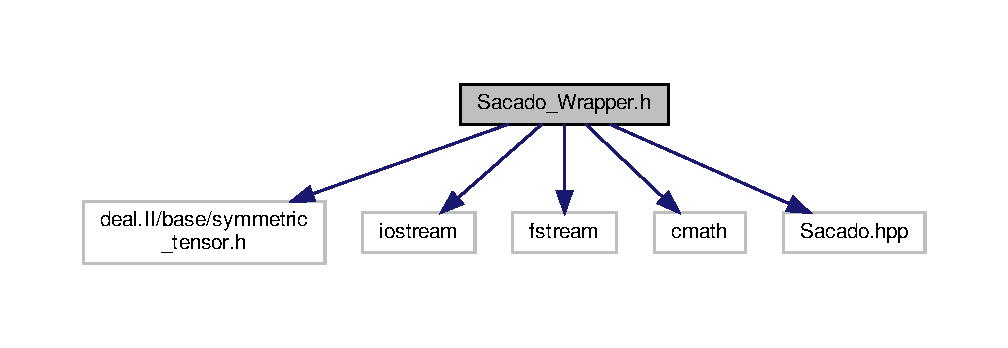
\includegraphics[width=350pt]{Sacado__Wrapper_8h__incl}
\end{center}
\end{figure}
This graph shows which files directly or indirectly include this file\+:
\nopagebreak
\begin{figure}[H]
\begin{center}
\leavevmode
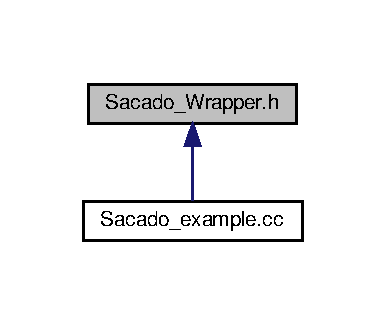
\includegraphics[width=185pt]{Sacado__Wrapper_8h__dep__incl}
\end{center}
\end{figure}
\subsection*{Classes}
\begin{DoxyCompactItemize}
\item 
class \hyperlink{classSacado__Wrapper_1_1SymTensor}{Sacado\+\_\+\+Wrapper\+::\+Sym\+Tensor$<$ dim $>$}
\item 
class \hyperlink{classSacado__Wrapper_1_1SymTensor2}{Sacado\+\_\+\+Wrapper\+::\+Sym\+Tensor2$<$ dim $>$}
\item 
class \hyperlink{classSacado__Wrapper_1_1SW__double}{Sacado\+\_\+\+Wrapper\+::\+S\+W\+\_\+double$<$ dim $>$}
\item 
class \hyperlink{classSacado__Wrapper_1_1SW__double2}{Sacado\+\_\+\+Wrapper\+::\+S\+W\+\_\+double2$<$ dim $>$}
\item 
class \hyperlink{classSacado__Wrapper_1_1DoFs__summary}{Sacado\+\_\+\+Wrapper\+::\+Do\+Fs\+\_\+summary$<$ dim $>$}
\end{DoxyCompactItemize}
\subsection*{Namespaces}
\begin{DoxyCompactItemize}
\item 
 \hyperlink{namespaceSacado__Wrapper}{Sacado\+\_\+\+Wrapper}
\end{DoxyCompactItemize}
\subsection*{Typedefs}
\begin{DoxyCompactItemize}
\item 
using \hyperlink{Sacado__Wrapper_8h_a868b94676739e612d9c95940e70892a9}{fad\+\_\+double} = Sacado\+::\+Fad\+::\+D\+Fad$<$ double $>$
\item 
typedef Sacado\+::\+Fad\+::\+D\+Fad$<$ double $>$ \hyperlink{Sacado__Wrapper_8h_a7e0893207b87dad05c66a34baac8ed2e}{D\+Fad\+Type}
\end{DoxyCompactItemize}
\subsection*{Functions}
\begin{DoxyCompactItemize}
\item 
{\footnotesize template$<$int dim$>$ }\\void \hyperlink{Sacado__Wrapper_8h_abe25ecefccdd45897ebc69797e1051ea}{get\+\_\+index\+\_\+map} (std\+::map$<$ unsigned \hyperlink{CMakeCache_8txt_a79a3d8790b2588b09777910863574e09}{int}, std\+::pair$<$ unsigned \hyperlink{CMakeCache_8txt_a79a3d8790b2588b09777910863574e09}{int}, unsigned \hyperlink{CMakeCache_8txt_a79a3d8790b2588b09777910863574e09}{int} $>$$>$ \&std\+\_\+map\+\_\+indicies)
\end{DoxyCompactItemize}


\subsection{Typedef Documentation}
\index{Sacado\+\_\+\+Wrapper.\+h@{Sacado\+\_\+\+Wrapper.\+h}!D\+Fad\+Type@{D\+Fad\+Type}}
\index{D\+Fad\+Type@{D\+Fad\+Type}!Sacado\+\_\+\+Wrapper.\+h@{Sacado\+\_\+\+Wrapper.\+h}}
\subsubsection[{\texorpdfstring{D\+Fad\+Type}{DFadType}}]{\setlength{\rightskip}{0pt plus 5cm}typedef Sacado\+::\+Fad\+::\+D\+Fad$<$double$>$ {\bf D\+Fad\+Type}}\hypertarget{Sacado__Wrapper_8h_a7e0893207b87dad05c66a34baac8ed2e}{}\label{Sacado__Wrapper_8h_a7e0893207b87dad05c66a34baac8ed2e}
\index{Sacado\+\_\+\+Wrapper.\+h@{Sacado\+\_\+\+Wrapper.\+h}!fad\+\_\+double@{fad\+\_\+double}}
\index{fad\+\_\+double@{fad\+\_\+double}!Sacado\+\_\+\+Wrapper.\+h@{Sacado\+\_\+\+Wrapper.\+h}}
\subsubsection[{\texorpdfstring{fad\+\_\+double}{fad_double}}]{\setlength{\rightskip}{0pt plus 5cm}using {\bf fad\+\_\+double} =  Sacado\+::\+Fad\+::\+D\+Fad$<$double$>$}\hypertarget{Sacado__Wrapper_8h_a868b94676739e612d9c95940e70892a9}{}\label{Sacado__Wrapper_8h_a868b94676739e612d9c95940e70892a9}


\subsection{Function Documentation}
\index{Sacado\+\_\+\+Wrapper.\+h@{Sacado\+\_\+\+Wrapper.\+h}!get\+\_\+index\+\_\+map@{get\+\_\+index\+\_\+map}}
\index{get\+\_\+index\+\_\+map@{get\+\_\+index\+\_\+map}!Sacado\+\_\+\+Wrapper.\+h@{Sacado\+\_\+\+Wrapper.\+h}}
\subsubsection[{\texorpdfstring{get\+\_\+index\+\_\+map(std\+::map$<$ unsigned int, std\+::pair$<$ unsigned int, unsigned int $>$$>$ \&std\+\_\+map\+\_\+indicies)}{get_index_map(std::map< unsigned int, std::pair< unsigned int, unsigned int >> &std_map_indicies)}}]{\setlength{\rightskip}{0pt plus 5cm}template$<$int dim$>$ void get\+\_\+index\+\_\+map (
\begin{DoxyParamCaption}
\item[{std\+::map$<$ unsigned {\bf int}, std\+::pair$<$ unsigned {\bf int}, unsigned {\bf int} $>$$>$ \&}]{std\+\_\+map\+\_\+indicies}
\end{DoxyParamCaption}
)}\hypertarget{Sacado__Wrapper_8h_abe25ecefccdd45897ebc69797e1051ea}{}\label{Sacado__Wrapper_8h_abe25ecefccdd45897ebc69797e1051ea}

\begin{DoxyCode}
23 \{
24     std::pair<unsigned int, unsigned int> tmp\_pair;
25 
26     \textcolor{keywordflow}{switch} ( dim )
27     \{
28     \textcolor{keywordflow}{case} 2:
29         tmp\_pair.first=0; tmp\_pair.second=0;
30         std\_map\_indicies[0] = tmp\_pair;
31 
32         tmp\_pair.first=0; tmp\_pair.second=1;
33         std\_map\_indicies[1] = tmp\_pair;
34 
35         tmp\_pair.first=1; tmp\_pair.second=1;
36         std\_map\_indicies[2] = tmp\_pair;
37         \textcolor{keywordflow}{break};
38     \textcolor{keywordflow}{case} 3:
39         tmp\_pair.first=0; tmp\_pair.second=0;
40         std\_map\_indicies[0] = tmp\_pair;
41 
42         tmp\_pair.first=0; tmp\_pair.second=1;
43         std\_map\_indicies[1] = tmp\_pair;
44 
45         tmp\_pair.first=0; tmp\_pair.second=2;
46         std\_map\_indicies[2] = tmp\_pair;
47 
48         tmp\_pair.first=1; tmp\_pair.second=1;
49         std\_map\_indicies[3] = tmp\_pair;
50 
51         tmp\_pair.first=1; tmp\_pair.second=2;
52         std\_map\_indicies[4] = tmp\_pair;
53 
54         tmp\_pair.first=2; tmp\_pair.second=2;
55         std\_map\_indicies[5] = tmp\_pair;
56         \textcolor{keywordflow}{break};
57     \}
58 \}
\end{DoxyCode}

%--- End generated contents ---

% Index
\backmatter
\newpage
\phantomsection
\clearemptydoublepage
\addcontentsline{toc}{chapter}{Index}
\printindex

\end{document}
